% !TeX spellcheck = en_US

\usetikzlibrary{math}

% Useful resources:
%   - https://github.com/cs231n/cs231n.github.io

\chapter{Introduction}
	This summary of the course "Deep Learning: Architectures and Methods" held at the TU Darmstadt covers a lot of topics in the wast field of deep learning and neural network architectures. The first part focuses on fully connected and convolutional networks and in the end some more advanced architectures are touched, namely recurrent, long short-term memory and transformer networks. Knowledge of basic machine learning taxonomy like "features", "training data" and "supervised learning" is assumed to be known as well as basic mathematical knowledge.

	The goal of deep architectures is learning a feature hierarchy where higher-level features are built on top of lower-level features. This is done by stacking multiple linear layers (perceptrons) on top of each other with nonlinearities between them to get a larger support. While it is, due to the universal function approximation theorem, not necessary to have multiple layers (one hidden layer is enough to approximate any sufficiently well-behaving function), it has been shown empirically that multiple layers improve the performance. In the last century the extreme computational power available leveraged the success of deep learning. This success was so extraordinary that deep learning became a hype that everyone jumped onto.

	This first chapter covers some milestones and history as well as the reason for the extreme success of deep learning.

	\section{Milestones}
		The first successful application of deep learning was in 1989 with LeNet to recognize zip codes. Image detection and classification was develop a lot further since that and in 2012, AlexNet broke the human prediction error on ImageNet, a collection of (then) \SI{200}{GB} labeled images. But deep learning is not only useful for image classification: In 2013, DeepMind beat the best human players on basic Arcade games and in 2016 AlphaGo defeated the world champion in the game Go. All of this was possible due to the massive power of deep neural networks and reinforcement learning.
	% end

	\section{The (Surprising?) Success of Deep Neural Networks}
		It is interesting that deep neural networks are so successful as they are built from extremely simple blocks. Also, the algorithms used for training these networks are extremely basic gradient descent descendants that only find local minima. In other words: they are greedy algorithms which are even more limited in what they can do than the network itself (if a problem has a greedy solution, it is usually regarded as an "easy" problem). But still they are extremely powerful!

		This is partially due to that hierarchical representations as induced by neural networks, are ubiquitous in artificial intelligence and information representation in general (e.g., images are hierarchical as well as natural language). Also, it seems like most learning problem are actually (relatively) easy and they have a gradient descent path towards a good model.
	% end
% end

\chapter{Optimization}
	\label{c:optimization}

	This chapter covers basic (numerical) optimization techniques that are used in machine and deep learning. Hence, it mainly focuses in gradient descent variants and less on, for example, sequential quadratic programming or trust region methods. A first method when thinking of optimization is a random search: instead of using sophisticated update rules for the parameters, they are sampled randomly. Obviously, this does not yield robust results and most often does not even yield any useful results. One advantage nevertheless is that random search does not get stuck in local minima and is, with infinite time, capable of finding the global optimum.

	\section{Gradient Descent}
		The basic idea of gradient descent (GD) is to follow the slope of the curve, i.e. the gradient\footnote{In this case the gradient refers to the vector of partial derivatives of a function w.r.t. all parameters.}. The gradient always points in the direction of the steepest \emph{ascent}, so its negative direction points towards the steepest descent. Intuitively, GD works like standing on a hill (the function that is being optimized) and always walking into the direction where the slope is the steepest. One might find the valley that way, but it is also possible to get stuck in a small hole. Formally the update equation for GD is given as
		\begin{equation}
			\vec{\theta}^{(k + 1)} = \vec{\theta}^{(k)} - \alpha \cdot \grad_{\vec{\theta}} L\bigl( \vec{\theta}^{(k)} \bigr),
		\end{equation}
		where \(\vec{\theta}\) are the parameters and \(L\) is the function to be minimized.

		\subsection{Evaluating the Gradient}
			As GD needs the values of the gradient, it has to be evaluated. There are three ways of approaching this: numerical evaluation, analytical derivatives or automatic differentiation.

			Numerical evaluation is extraordinarily simple, but is only approximate and slow to evaluate (when using forward difference quotients, the function has to be evaluated two times for each parameter).

			Analytical derivatives is hard and time-consuming, but exact and fast. But it is also error-prone as both the original function and the derivative have to be both implemented and derived. To verify that an analytical gradient is correct one method used in practice is to also evaluate the gradient numerically and checking if the results are roughly equal.

			As neural networks usually have lots of parameters and are fairly complex computational structures, neither of these methods are practical. Hence, automatic differentiation is used. In automatic differentiation, a computational graph is built and then the gradients are propagated backwards through it. This is called backpropagation and is covered in more detail in \autoref{c:backpropagation}.
		% end

		\subsection{Mini-Batch and Stochastic Gradient Descent}
			In mini-batch GD, only a small portion (common sizes are \num{32}, \num{64}, or \num{128} samples) of the training set is used for computing the gradient. This technique is used as it might not be possible to compute the whole gradient due to memory limitations. This makes the gradient noisy, but the progress is still good on average. It is also called \emph{stochastic} GD as the gradient gets replaced by a Monte-Carlo estimate of the expectation of the gradient.
		% end
	% end

	\section{Newton's Method and L-BFGS}
		Instead of walking along the gradient, \emph{Newton's method} leverages further knowledge from calculus and uses not only the gradient but the Hessian, too. The update equation is
		\begin{equation}
			\vec{\theta}^{(k + 1)} = \vec{\theta}^{(k)} - \alpha \cdot \Bigl(\!\mat{H}_L\bigl( \vec{\theta}^{(k)} \bigr)\!\Bigr)^{-1} \, \grad_{\vec{\theta}} L\bigl( \vec{\theta}^{(k)} \bigr),
		\end{equation}
		where \(\mat{H}_L\) is the Hessian. Newton's method is capable of finding the minima of quadratic functions in one step and also converges fast for other problems. But due to its dependence on the Hessian, which is costly to compute, and due to the inverse of the said, it is rarely used in deep learning. The inversion has a time complexity of \( \mathcal{O}(d^3) \), where \(d\) are the number of parameters. As neural networks usually have millions of parameters, inverting the matrix is not practical. Also, matrix inversion is numerically unstable and the Hessian might even be singular.

		Arising from these problems, the L-BFGS algorithm was developed which directly approximates the inverse of the Hessian. Hence, neither calculating nor inverting it is necessary.
	% end

	\section{Convergence}
		A method is said to converge \emph{quadratically} if the error \( \epsilon_k = x_\ast - x \) depends quadratically on the previous error:
		\begin{equation}
			\epsilon_{k + 1} = \mu \epsilon_k^2,\qquad \epsilon_k \in \mathcal{O}\bigl(\mu^{2^k}\bigr)
		\end{equation}
		Analogously, a method converges \emph{linearly} if the error depends linearly on the previous error:
		\begin{equation}
			\epsilon_{k + 1} \leq \mu \epsilon_k,\qquad \epsilon_k \in \mathcal{O}(\mu^n)
		\end{equation}
		For SGD, when the learning rate is changed to \(1/n\), the convergence is \( \epsilon_k \in \mathcal{O}(1/n) \). So SGD is terrible compared to other methods, but still it is used in practice as one million iterations or so are still enough for reaching single point precision in the error and one million iterations are okay to compute.
	% end

	\section{Momentum}
		When using SGD, the trajectory along the algorithm converges is very jittery on steep locations as the gradient is large and huge steps are made. On the other hand, only very slow progress is made at locations where the gradient is small. One approach for tackling this problem is \emph{momentum}. The formal definition is
		\begin{align}
			\vec{v}^{(k + 1)} &= \mu \vec{v}^{(k)} - \alpha \cdot \grad_{\vec{\theta}} L\bigl(\vec{\theta}^{(k)}\bigr) \\
			\vec{\theta}^{(k + 1)} &= \vec{\theta}^{(k)} + \vec{v}^{(k + 1)}
		\end{align}
		with a "friction" coefficient \(\mu\) which is usually \num{0.5}, \num{0.9}, or \num{0.99} or annealed over time (e.g., from \num{0.5} to \num{0.99}). The intuition is that the gradient can build up velocity along shallow regions of the loss which gets damped in steep regions. This reduces the jittering at steep regions by reducing the size of the gradients and ramps up the speed on shallow regions.

		The momentum is usually initialized with zeros.

		\subsection{Nesterov Momentum}
			A variant of the vanilla momentum is \emph{Nesterov momentum}, where the update is compute "one step ahead" by following the old momentum:
			\begin{align}
				\vec{v}^{(k + 1)} &= \mu \vec{v}^{(k)} - \alpha \cdot \grad_{\vec{\theta}} L\bigl( \vec{\theta}^{(k)} + \mu \vec{v}^{(k)} \bigr) \\
				\vec{\theta}^{(k + 1)} &= \vec{\theta}^{(k)} + \vec{v}^{(k + 1)}
			\end{align}
			Notice the change in the top equation when calculating the gradient. But this calculation is slightly inconvenient as usually the forward pass is computed for the current parameter settings anyway, e.g., for computing the predication accuracy. This inconvenience can be circumvented by a slight change of variables. Setting \( \vec{\phi}^{(k)} = \vec{\theta}^{(k)} + \mu \vec{v}^{(k)} \) and rearranging the formulas a bit, the update equation becomes:
			\begin{align}
				\vec{v}^{(k + 1)} &= \mu \vec{v}^{(k)} - \alpha \cdot \grad_{\vec{\theta}} L\bigl(\vec{\phi}^{(k)}\bigr) \\
				\vec{\phi}^{(k + 1)} &= \vec{\phi}^{(k)} - \mu \vec{v}^{(k)} + (1 + \mu) \vec{v}^{(k + 1)}
			\end{align}
			The disadvantage of this change of variables is that now the previous value of the momentum has to be kept in memory, but this is mainly an implementation pitfall one has to care for.
		% end

		\subsection{AdaGrad}
			Another variant of SGD is \emph{AdaGrad} which changes the update in a ways such that the gradients are normalized by the square-root of gradient norms. This reduces the learning rate when gradients are high and increases it when gradients are small. Hence, the algorithms moves faster in shallow and slower in steep regions:
			\begin{align}
				s^{(k + 1)} &= s^{(k)} + \Big\lVert \grad_{\vec{\theta}} L\bigl(\vec{\theta}^{(k)}\bigr) \Big\rVert_2^2 \\
				\vec{\theta}^{(k + 1)} &= \vec{\theta}^{(k)} - \frac{\alpha}{\sqrt{s^{(k + 1)}} + \epsilon} \grad_{\vec{\theta}} L\bigl(\vec{\theta}^{(k)}\bigr)
			\end{align}
			The "gradient cache" \(s\) is initialized with zero and \(\epsilon\) is a small number added to the denominator to prevent divisions by zero. Problems of AdaGrad are that the first step can be far off and that the learning rate vanishes over time due to \(s\) building up large values (as norms can never be negative), causing learning to stagnate.
		% end

		\subsection{RMSProp}
			\emph{RMSProp} tackles the problem of AdaGrad that the learning rate vanishes by adding a decay rate \(\eta \in [0, 1)\) to it:
			\begin{align}
				s^{(k + 1)} &= s^{(k)} \beta s^{(k)} + (1 - \beta) \big\lVert \grad_{\vec{\theta}} L\bigl(\vec{\theta}^{(k)}\bigr) \big\rVert_2^2 \\
				\vec{\theta}^{(k + 1)} &= \vec{\theta}^{(k)} - \frac{\alpha}{\sqrt{s^{(k + 1)}} + \epsilon} \cdot \grad_{\vec{\theta}} L\bigl(\vec{\theta}^{(k)}\bigr)
			\end{align}
			With a decay of \( \beta = 0 \), RMSProp is equivalent to AdaGrad. The decay rate should be set to something high like \( \beta = 0.9 \) as small learning rates cause exploding updates in the first steps. Like for AdaGrad, the first few steps can be quite far off.
		% end

		\subsection{Adam}
			\emph{Adam} is the state-of-the-art optimizer used nearly every time for training neural networks. It combines the idea of momentum with RMSProp
			\begin{align}
				\vec{v}^{(k + 1)} &= \beta_1 \vec{v}^{(k)} + (1 - \beta_1) \cdot \grad_{\vec{\theta}} L\bigl(\vec{\theta}^{(k)}\bigr) \\
				s^{(k + 1)} &= \beta_2 s^{(k)} + (1 - \beta_2) \big\lVert \grad_{\vec{\theta}} L\bigl(\vec{\theta}^{(k)}\bigr) \big\rVert_2^2 \\
				\hat{\vec{v}}^{(k + 1)} &= \frac{\vec{v}^{(k + 1)}}{1 - \beta_1^{k + 1}} \\
				\hat{s}^{(k + 1)} &= \frac{s^{(k + 1)}}{1 - \beta_2^{k + 1}} \\
				\vec{\theta}^{(k + 1)} &= \vec{\theta}^{(k)} - \frac{\alpha}{\sqrt{\hat{s}^{(k + 1)}} + \epsilon} \vec{v}^{(k + 1)}
			\end{align}
			where the hatted variables are a bias correction that compensates for the zero-initialization of \(\vec{v}\) and \(s\) and only really affects the process in the first few iterations where \(k\) i small.
		% end
	% end

	\section{Learning Rate}
		All of the above optimizers share at least one hyperparameter: the learning rate \(\alpha\). This hyperparameter is usually the one with the most influence on the learning process. If the learning rate is too small, no learning happens. But if it is too high, the parameters blow up and the loss rises indefinitely. A good learning rate is somewhere im between. Tuning of the learning rate and hyperparameter search will also be covered in \autoref{subsec:hyperparameterOpt}.

		As usually most learning happens in the beginning and later on fine-tuning happens, it can be useful to decay the learning rate over time, i.e., make \(\alpha\) \(k\)-dependent: \(\alpha_k\). Two options are exponential decay
		\begin{equation}
			\alpha_k = \alpha_0 e^{-\eta k}
		\end{equation}
		with an initial learning rate \(\alpha_0\) and a decay rate \(\eta\). Another option is \(1/k\)-decay
		\begin{equation}
			\alpha_k = \frac{\alpha_0}{1 + \eta k},
		\end{equation}
		again with an initial learning rate \(\alpha_0\) and a decay rate \(\eta\). Other options are for example step-based decay (e.g., every \(n\) iterations, go done by a factor) or even manual decay.
	% end
% end

\chapter{Backpropagation}
	\label{c:backpropagation}

	As already discussed in \autoref{c:optimization}, the gradient of the loss function has to be computed in order to update the parameters of a neural network. The best method for doing this is automatic differentiation which is both fast (compared to numerical evaluation) and not as error-prone as analytical derivatives which have to be both implemented and derived by hand. The heart of automatic differentiation is building a computational graph and applying the chain rule
	\begin{equation}
		\dv{x} f\bigl( g(x) \bigr) = \pdv{f\bigl( g(x) \bigr)}{g(x)} \dv{g(x)}{x}
	\end{equation}
	multiple times. As an example \autoref{fig:compGraph} shows the computational graph for \( \bigl( (x + y) z \bigr)^2 \), including a forward pass (for computing the output) as well as a backward pass (for computing the derivatives). Computing the derivative goes as follows: start with one on the output (this is the derivative of the output w.r.t. the output). Then subsequently compute the local derivatives for each node with respect to the node the edge is coming from. This local derivative is then multiplied with the \emph{upstream gradient}, i.e., the value of the derivative coming in from the right. This yields the derivative of the output w.r.t. the node the edge the current number is computed for is coming from.

	This exhibits some interesting properties of the gradient flow and the patterns several gates induce. First of all, an add gate distributes the gradient between the incoming paths:
	\begin{align}
		\pdv{x} (x + y) &= 1 &
		\pdv{y} (y + y) &= 1
	\end{align}
	A product gate "switches" the gradient as the first downstream gradient gets multiplied by the value of the second flow:
	\begin{align}
		\pdv{x} (xy) &= y &
		\pdv{y} (xy) &= y
	\end{align}
	Another interesting gate is the max gate which "routes" the gradient depending on the input values, i.e., the gradient of which the flow has the smaller variable vanishes:
	\begin{align}
		\pdv{x} \max(x, y) &=
			\begin{cases}
				1 & \text{if } x > y \\
				0 & \text{if } x < y
			\end{cases} &
		\pdv{y} \max(x, y) &=
			\begin{cases}
				0 & \text{if } x > y \\
				0 & \text{if } x < y
			\end{cases}
	\end{align}
	An important property here is that the derivative for \(x = y\) is undefined as the maximum is not differentiable for \(x = y\). In practice, however, exact equality is rarely the case so this is not a real problem. Similarly a ReLU \( \max(0, x) \) works like a gradient switch where it can only pass through if the value was positive during the forward pass.

	In is also possible go forward through the network. This is called \emph{forward differentiation} opposed to \emph{backward differentiation}. In forward differentiation, the derivative \( \pdv*{x}{y} \) is computed, in backward differentiation the derivative \( \pdv*{y}{x} \) is computed. As neural networks usually have a scalar loss as the output, backward differentiation is trivial and easy to calculate.

	In real-world application, the backward pass would be computed in a batched/vectorized fashion for multiple input/output data and weights at once. This can be implemented efficiently using Einstein summation. \autoref{lst:forwardBackwardPass} shows a forward- and backward-pass through a multi-layer perceptron with two hidden layers and sigmoid nonlinearities after each hidden layer and no output nonlinearity.

	\begin{figure}
		\centering
		\begin{tikzpicture}[->, comp/.style = { draw, circle, minimum width = 0.8cm, minimum height = 0.8cm, inner sep = 0 }]
			\node (x) {\(x\)};
			\node [below = 1 of x] (y) {\(y\)};
			\node [below = 1 of y] (z) {\(z\)};
			\node [comp, right = 3 of x, label = above:{\(a\)}] (c1) {\(+\)};
			\node [comp, right = 3 of c1, label = above:{\(b\)}] (c2) {\(\ast\)};
			\node [comp, right = 3.5 of c2, label = above:{\(c\)}] (c3) {\(\cdot^2\)};
			\coordinate [right = 2 of c3] (c4);

			\draw (x) -- node[above, sloped, near start]{\(2\)} node[below, sloped, near start]{\(160\)} (c1);
			\draw (y) -- node[above, sloped, near start]{\(3\)} node[below, sloped, near start]{\(160\)} (c1);
			\draw (z) -- node[above, sloped]{\(4\)} node[below, sloped]{\( \pdv{c}{z} = \pdv{c}{b} \pdv{b}{c} = 40 \cdot a = 40 \cdot 5 = 200 \)} (c2);
			\draw (c1) -- node[above, sloped, near start]{\(5\)} node[below, sloped, near start]{\(160\)} (c2);
			\draw (c2) -- node[above, sloped]{\(20\)} node[below, sloped]{\(\pdv{c}{b} = \pdv{c}{c} \pdv{c}{b} = 1 \cdot 40\)} (c3);
			\draw (c3) -- node[above, sloped]{\(400\)} node[below, sloped]{\(\pdv{c}{c} = 1\)} (c4);
		\end{tikzpicture}
		\caption{Computational graph for \( \bigl( (x + y) z \bigr)^2 \). The numbers above the edges represent the forward pass, the numbers below the edges the backward pass (the derivatives). For some edges the application of the chain rule is written out explicitly. All other edges get computed analogous.}
		\label{fig:compGraph}
	\end{figure}

	\begin{lstlisting}[
			language = Python,
			caption = {Forward- and backward-pass for a multi-layer perceptron.},
			label = lst:forwardBackwardPass
		]
# W1, W2, W3, b1, b2, b3 are the weights/biases of the layers.
hid_1 = sigmoid(W1 @ X + b1[:, np.newaxis])
hid_2 = sigmoid(W2 @ hid_1 + b2[:, np.newaxis])
outputs = W3 @ hid_2 + b3[:, np.newaxis]

dL  = deriv_squared_loss(outputs, targets)
dW3 = np.einsum('ib,jb->ij', dL, hid_2)
db3 = np.einsum('ib->i', dL)

dS2 = deriv_sigmoid(W2 @ hid_1 + b2[:, np.newaxis])
dL  = np.einsum('kb,ki,ib->ib', dL, W3, dS2)
dW2 = np.einsum('ib,jb->ij', dL, hid_1)
db2 = np.einsum('ib->i', dL)

dS1 = deriv_sigmoid(W1 @ X + b1[:, np.newaxis])
dL  = np.einsum('kb,ki,ib->ib', dL, W2, dS1)
dW1 = np.einsum('ib,jb->ij', dL, X)
db1 = np.einsum('ib->i', dL)
	\end{lstlisting}

	\section{Activation Functions}
		\label{sec:activationFunctions}

		The \emph{activation function} is the nonlinearity behind a linear layer of a neural network, enriching the prediction power of the network. The big problem with activation functions is that---as neural networks lack interpretability---it is not really known what nonlinearities are good for which task. This section discusses some of the most popular activation functions and their respective pros and cons.

		\subsubsection{Sigmoid}
			One of the first activation functions was \emph{sigmoid} which squashes all input numbers into a range from zero to one:
			\begin{align}
				\sigma : \R \to (0, 1) : x \mapsto \frac{1}{1 + e^{-x}} &&
				\sigma'(x) = \sigma(x) \bigl( 1 - \sigma(x) \bigr)
			\end{align}
			Sigmoid is best for learning logical inputs, i.e., functions with binary inputs and is used for control signals in LSTM networks. But they can kill gradients for values \( \lvert x \rvert \lg 0 \) as the derivative is near zero for values far away from the center. Sigmoid is also not good for image networks (better use ReLU) and is not zero-centered. The latter is a problem because the sigmoid itself requires zero-centered input data for producing non-trivial (constant) results.

			Additionally, an always-positive input to a neuron causes the gradients to always be all-positive or all-negative. this leads to a zigzag path through the parameter space (much like axial iteration) which is not near an optimal optimization trajectory. This is also why the input data shall always be zero-centered beforehand (i.e., the mean of the input data should be zero).
		% end

		\subsubsection{Hyperbolic Tangent (Tanh)}
			The shape of the \emph{hyperbolic tangent} (tanh) activation function is similar, but the numbers are squashed into a range from plus to minus one:
			\begin{align}
				\tanh : \R \to (-1, 1) : x \mapsto \frac{e^x - e^{-x}}{e^x + e^{-x}} &&
				\tanh'(x) = 1 - \tanh^2(x)
			\end{align}
			Much like the sigmoid, gradients are killed for \(x\) values away from zero. But as the output is zero-centered, the tanh activation function is better suited for most problems as opposed to the sigmoid. It is also used for bounded, but signed, values in LSTM networks. But they are not as good as sigmoid for binary functions.
		% end

		\subsubsection{Rectified Linear Unit (ReLU)}
			The \emph{Rectified Linear Unit} (ReLU) is (at the moment) the go-to activation function for most problems:
			\begin{align}
				\mathrm{ReLU} : \R \to [0, \infty) : x \mapsto \max(0, x) &&
				\mathrm{ReLU}'(x) =
					\begin{cases}
						1 & \text{if } x > 0 \\
						0 & \text{if } x < 0
					\end{cases}
			\end{align}
			It saturates on half of the real axis and kills the gradient there, but it does never kill the gradient on the other half and is thus better suited for most problems than sigmoid or tanh. This is also visible empirically: networks using ReLU activations converge around six times faster than networks using sigmoid/tanh activations. But it is also not suitable for logical functions or for control in recurrent networks. Also, the output is not zero-centered. Another (theoretical) problem is that the gradient at \(x = 0\) is not defined. In practice this is not a big problem as values are almost never exactly equal to zero. If they are, one usually chooses zero or one as a gradient value, it does not really matter.

			To prevent the gradients from dying (a saturated ReLU is often called a \emph{dead ReLU}), the network is usually initialized with a slightly positive bias (e.g., \num{0.01}).
		% end

		\subsubsection{Leaky and Parametric ReLU}
			An alternative to the vanilla ReLU are the \emph{leaky} and \emph{parametric} ReLU. The parametric ReLU is given as
			\begin{align}
				\mathrm{PReLU}_\alpha : \R \to (-\infty, \infty) : x \mapsto \max(\alpha x, x) &&
				\mathrm{PReLU}_\alpha'(x) =
					\begin{cases}
						1      & \text{if } x > 0 \\
						\alpha & \text{if } x < 0
					\end{cases}
			\end{align}
			where for the leaky ReLU the parameter is fixed to \( \alpha = 0.01 \). This parameter is also learnable. Compared to all activation functions discussed before, the leaky and parametric ReLU do not saturate and have most advantages of the ReLU (e.g., faster convergence than sigmoid/tanh). Also the outputs are closer to zero-mean compared to a vanilla ReLU. But it is still not differentiable at \( x = 0 \).
		% end

		\subsubsection{Exponential Linear Unit (ELU)}
			The \emph{exponential linear unit} (ELU) combines the pros of a ReLU with differentiability at \(x = 0\):
			\begin{align}
				\mathrm{ELU} : \R \to (-\alpha, \infty) : x \mapsto
					\begin{cases}
						x                          & \text{if } x > 0    \\
						\alpha \big( e^x - 1 \big) & \text{if } x \leq 0
					\end{cases} &&
				\mathrm{ELU}'(x) =
					\begin{cases}
						\alpha e^x & \text{if } x > 0 \\
						1          & \text{if } x < 0 \\
						1          & \text{if } x = 0 \text{ and } \alpha = 1
					\end{cases}
			\end{align}
			As can be seen from the derivative, if \(\alpha = 1\) is chosen, the function is continuously differentiable everywhere. Otherwise it is not differentiable at \(x = 0\). The value of \(\alpha\) defines the value of the ELU as \(x \to -\infty\).
		% end

		\subsubsection{Maxout Neuron}
			The \emph{maxout neuron} is a special kind of neuron that combines the weighting and bias with the activation function:
			\begin{align}
				\max\bigl( \vec{w}_1^T \vec{x} + b_1,\, \vec{w}_2^T \vec{x} + b_2 \bigr)
			\end{align}
			It generalizes the parametric ReLU and works in the linear regime, and hence does not saturate. But it has the problem that it doubles the number of parameters as two weight matrices and biases have to be used.
		% end

		\subsubsection{In Practice\dots}
			\dots everything should be tried, usually ReLU. But also try leaky ReLU, Maxout and ELU. For binary (logical) functions, use sigmoid and also try out tanh (but do not hope for much).
		% end
	% end

	\section{Regularization}
		The number of layers and neurons per layer has an extreme impact on the performance and capacity of a network. In general more layers work better over more neurons per layer and more layers/neurons in general work better than less. But large networks can lead to overfitting when there are a lot more parameters then there is data! But instead of regularizing the network using the network size, it is better to use a strong regularization on the weights instead, e.g., L1- or L2-regularization. In these regularization methods, the sum of the absolute (L1) or squared (L2) weights is added to the loss with a penalty factor \(\lambda\) (usually \num{0.1}, \num{0.01}, or \num{0.001}). This keeps the parameters small and thus reduces model complexity.
	% end
% end

\chapter{Training Neural Networks}
	This chapter covers the complete learning process of neural networks. Some quirks and tricks for data pre-processing and normalization are covered as well as hyperparameter optimization and regularization.

	% TODO: Training Neural Networks: History; 4.24, 4.25, 4.26, 4.27, 4.28

	\section{Data Pre-Processing: Normalization}
		As already seen during the discussion of activation functions in \autoref{sec:activationFunctions}, it is desirable to have zero-centered input data, i.e., data with a zero mean. Because of that it is common (and recommended) to first \emph{normalize} the input data before training by subtracting the mean. Additionally the data is also often \emph{standardized}, meaning the normalized data is divided by the standard deviation of all samples to get a variance of one in every direction. This way the data does not fluctuate much along all axis which eases the training. It is also common to \emph{whiten} the data by applying a PCA (Principal Component Analysis) transformation to it, producing a unit Gaussian and decorrelating the features by rotating the data (such that the covariance matrix is the identity matrix).

		For images, however, it is common to not standardize or whiten the data but to just subtract the mean (e.g. the mean image in AlexNet of the per-channel mean in VGGNet). This is due to the numbers of an image being bounded by nature, e.g. to the interval from zero to one. Hence different variances along the different axis might even encode information that shall not be removed.

		During test time, the test input data has to be shifted and scaled the same way the training data was, based on the mean/standard deviation/PCA matrix/\dots that was computed from the training data. So the mean is not re-computed during test time!
	% end

	\section{Weight Initialization}
		An important factor of training neural networks is the initialization of the weights and biases in the neurons. If, for example, all weights are initialized with zeros, all downstream gradients vanish as they get multiplied with the weights. Hence, no learning happens. Besides the methods proposed below, initialization remains an open topic in neural network research and is not well understood. What is well understood, however, is that initialization plays a really important role and more often than expected is the key factor for the success of a neural network\footnote{Jonathan Frankle and Michael Carbin (2018): "The Lottery Ticket Hypothesis: Finding Sparse, Trainable Neural Networks"}.

		\paragraph{Small or Big Random Numbers}
			Another idea is to initialize all weights by sampling from a Gaussian distribution with a small standard deviation, e.g. \( \sigma = 0.01 \). This works fine for small networks, but for deep networks this initialization causes the mean and standard deviation of the activations in each layer to collapse quickly to zero. This is due to multiple small numbers getting multiplied together a lot of times. But activations with (near) zero values cause the gradient of the weights to vanish! Like for an initialization with all zeros, this causes no learning to happen.

			So small numbers are not the key to success. On the other hand, using a variance of \( \sigma = 1 \) for generating the initial weights does not work out either because the activation functions saturate quickly, yielding vanishing gradients. Hence again, no learning happens. For ReLU, this can also lead to exploding values as ReLU is not bounded.

			\autoref{fig:nnInitSmallRandom} shows the activation statistics of random data propagating through a ten-layer neural network with \num{300} neurons each. It can be seen that the mean and standard deviation saturate quickly, characterized by the histograms getting sharper. \autoref{fig:nnInitBigRandom} shows the same kind of plot, but for the big standard deviation. In this case the ReLU activation function is not shown in the mean/standard deviation plots because it blows up exponentially. But for sigmoid and tanh it can be seen that they saturate, too, causing the gradients to vanish.

			\begin{figure}
				\centering
				\begin{subfigure}{\linewidth}
					\includegraphics[width=\linewidth]{tmp-nn-init-normal-small.pdf}
					\caption{Mean and standard deviation in each layer.}
				\end{subfigure}
				\begin{subfigure}{\linewidth}
					\includegraphics[width=\linewidth]{tmp-nn-init-normal-small-Sigmoid-hist.pdf}
					\caption{Histogram of the values in each layer for the sigmoid activation function.}
				\end{subfigure}
				\begin{subfigure}{\linewidth}
					\includegraphics[width=\linewidth]{tmp-nn-init-normal-small-Tanh-hist.pdf}
					\caption{Histogram of the values in each layer for the tanh activation function.}
				\end{subfigure}
				\begin{subfigure}{\linewidth}
					\includegraphics[width=\linewidth]{tmp-nn-init-normal-small-ReLU-hist.pdf}
					\caption{Histogram of the values in each layer for the ReLU activation function.}
				\end{subfigure}
				\caption{Activation statistics for weights initialized by a Gaussian with small variance. Layer zero is the input layer. For all activation functions it can be seen that the mean saturates quickly and the standard deviation vanishes.}
				\label{fig:nnInitSmallRandom}
			\end{figure}

			\begin{figure}
				\centering
				\begin{subfigure}{\linewidth}
					\includegraphics[width=\linewidth]{tmp-nn-init-normal-big.pdf}
					\caption{Mean and standard deviation in each layer.}
				\end{subfigure}
				\begin{subfigure}{\linewidth}
					\includegraphics[width=\linewidth]{tmp-nn-init-normal-big-Sigmoid-hist.pdf}
					\caption{Histogram of the values in each layer for the sigmoid activation function.}
				\end{subfigure}
				\begin{subfigure}{\linewidth}
					\includegraphics[width=\linewidth]{tmp-nn-init-normal-big-Tanh-hist.pdf}
					\caption{Histogram of the values in each layer for the tanh activation function.}
				\end{subfigure}
				\begin{subfigure}{\linewidth}
					\includegraphics[width=\linewidth]{tmp-nn-init-normal-big-ReLU-hist.pdf}
					\caption{Histogram of the values in each layer for the ReLU activation function.}
				\end{subfigure}
				\caption{Activation statistics for weights initialized by a Gaussian with big variance. Layer zero is the input layer. For all activation functions it can be seen that the neurons saturates quickly. The standard deviation is not zero, but this is caused by the sigmoid and tanh activation to have two saturation values.}
				\label{fig:nnInitBigRandom}
			\end{figure}
		% end

		\paragraph{Xavier Initialization}
			\emph{Xavier initialization} also uses normally distributed weights, but the standard deviation is reciprocally proportional to the square-root of the number of neurons in the previous layer (called \emph{fan in}): \( \sigma = 1/\sqrt{\textit{fan-in}} \). This is a reasonable activation and works well when using sigmoid or tanh activations. But when using ReLU activations, the gradients vanish again as nearly all activations get saturated in the left half of the ReLU (where it is flat). Instead, He et al. (2015) proposed to divide the fan in by two to get a better initialization, i.e., \( \sigma = 1/\sqrt{\textit{fan-in} / 2} \). This works reasonably well also for ReLU activations.

			\autoref{fig:nnInitXavier} shows the activation statistics like before. For tanh the mean approaches zero, but this is a good thing as zero-centered data reduces saturation in the next layer as long as the histogram is sufficiently wide. But it does not work good for ReLU which saturates quickly. The alternative Xavier initialization proposed by He et al. is shown in \autoref{fig:nnInitHe}, yielding similar results for sigmoid and tanh. But even for the ReLU, the histogram is not as sharp as for vanilla Xavier initialization.

			\begin{figure}
				\centering
				\begin{subfigure}{\linewidth}
					\includegraphics[width=\linewidth]{tmp-nn-init-xavier.pdf}
					\caption{Mean and standard deviation in each layer.}
				\end{subfigure}
				\begin{subfigure}{\linewidth}
					\includegraphics[width=\linewidth]{tmp-nn-init-xavier-Sigmoid-hist.pdf}
					\caption{Histogram of the values in each layer for the sigmoid activation function.}
				\end{subfigure}
				\begin{subfigure}{\linewidth}
					\includegraphics[width=\linewidth]{tmp-nn-init-xavier-Tanh-hist.pdf}
					\caption{Histogram of the values in each layer for the tanh activation function.}
				\end{subfigure}
				\begin{subfigure}{\linewidth}
					\includegraphics[width=\linewidth]{tmp-nn-init-xavier-ReLU-hist.pdf}
					\caption{Histogram of the values in each layer for the ReLU activation function.}
				\end{subfigure}
				\caption{Activation statistics for weights initialized using Xavier initialization. Layer zero is the input layer. Except for the ReLU activation, Xavier initialization works well and the neurons do not saturate.}
				\label{fig:nnInitXavier}
			\end{figure}

			\begin{figure}
				\centering
				\begin{subfigure}{\linewidth}
					\includegraphics[width=\linewidth]{tmp-nn-init-he.pdf}
					\caption{Mean and standard deviation in each layer.}
				\end{subfigure}
				\begin{subfigure}{\linewidth}
					\includegraphics[width=\linewidth]{tmp-nn-init-he-Sigmoid-hist.pdf}
					\caption{Histogram of the values in each layer for the sigmoid activation function.}
				\end{subfigure}
				\begin{subfigure}{\linewidth}
					\includegraphics[width=\linewidth]{tmp-nn-init-he-Tanh-hist.pdf}
					\caption{Histogram of the values in each layer for the tanh activation function.}
				\end{subfigure}
				\begin{subfigure}{\linewidth}
					\includegraphics[width=\linewidth]{tmp-nn-init-he-ReLU-hist.pdf}
					\caption{Histogram of the values in each layer for the ReLU activation function.}
				\end{subfigure}
				\caption{Activation statistics for weights initialized using the modified Xavier initialization by He et al. Layer zero is the input layer. It can be seen that the histograms in the layers are sufficiently wide, enabling learning. Also the ReLU does not saturate.}
				\label{fig:nnInitHe}
			\end{figure}
		% end

		\subsection{Batch Normalization}
			As already seen, unit Gaussian data is best as an input for most activation functions. The idea of batch normalization to just make the data unit Gaussian by subtracting the mean and dividing by the (empirical) standard deviation at each layer. This is done by averaging the incoming data along each dimension and computing the standard deviation for each dimension. Then element-wise subtraction and division is used for normalize and standardize the data. As the network then learns weights and biases on this data, it is theoretically possible that the networks learns to recover the original data by learning the values of the mean and standard deviation. Hence, no prediction power is taken away from the network by adding a batch normalization layer\footnote{Note that this is just a semi-theoretical argument to support batch normalization. In practice, the neural network nearly never learns the mean and standard deviation}.

			Advantages of batch normalization is that it improves the gradient flow through the network, allows higher learning rates by high-quality gradients, and reduces the strong dependence on initialization. It also kind of works as a form of regularization and maybe reduces the need for dropout.

			During test time, the mean and standard deviation that were computed during training are used to normalizing/standardizing the data---the test data is not used to compute the mean/standard deviation again.
		% end
	% end

	\section{Designing a Network and Hyperparameter Optimization}
		This section covers the basic steps of designing a neural network, i.e., choosing the architecture, the loss, etc. The first step is to pre-process the data (normalization) as this is usually useful. The next step is to choose the architecture. This heavily depends on the task and prior intuition and knowledge are extremely helpful for settings up a good initial network. Furthermore, double check that the loss is reasonable: do not use cross-entropy for regression or quadratic loss for classification and remember to disable any regularization tricks. When enabling regularization, the loss should go up---that can be checked, too.

		The next step is to train the network on a small portion of the training data to see if the model can overfit. If the model is not able to overfit on a very small dataset, its capacity is not high enough and the neural network has to be made larger. If that works, switch to training on the complete dataset and tuning of the learning rate. If the loss is not going down, the learning rate is usually too low. If the loss is exploding, the learning rate is usually too high. A principled way of finding a good learning rate is to use cross-validation on several learning rates that are magnitudes apart (a learning rate of \(0.0002\) usually performs similar to \(0.0001\), so try out \(0.1\), \(0.01\), \(0.001\), \dots). This boils down to hyperparameter optimization as the learning rate is a hyperparameter.

		\section{Hyperparameter Optimization}
			\label{subsec:hyperparameterOpt}

			\emph{Hyperparameter optimization} is a big topic in designing neural networks and deep learning in general. It usually boils down to trying out different hyperparameter settings in a principled way. As a first step, a coarse search for only a few epochs should be done to get a rough idea what parameter settings work. Afterwards, a finer search for more iterations is executed to get more precise parameters. To speed up this process it is often advisable to stop the learning if the loss gets more than three times as high as the original loss. Also, the update ratio, i.e., the ratio between the norm of the old weights and the norm of the new weights \( \lVert \vec{\theta}^{(k)} \rVert_2 / \lVert \vec{\theta}^{(k + 1)} \rVert_2 \), should be around \num{0.001} or so.

			For the coarse search it is best to search in log-space. This is especially true for the learning rate which is the most important parameter. Other hyperparameters to try are for example the network architecture itself, the decay schedule of the learning rate and its update type, regularization (L2/dropout strength), etc. When looking at the accuracy, there should also be a small gap between the training and test accuracy. If the gap is too big, the model overfitted and the regularization strength should be increased. If these is no gap, the model capacity is most likely too low and the network should be enlarged.

			\subsection{Grid vs. Random Search}
				When evaluating multiple parameters at once, it is advisable to not evaluate them on a grid, but to sample each from a uniform distribution. It is often the case that one hyperparameter (e.g. the learning rate) has a higher influence on the result than another (e.g. the initialization of the bias). If one uses a grid, a lot of redundant computations will be performed for a single parameter. When using random values, this happens less frequent. This is illustrated in \autoref{fig:gridRandomSearch}.

				\begin{figure}
					\centering
					\begin{subfigure}{0.49\linewidth}
						\centering
						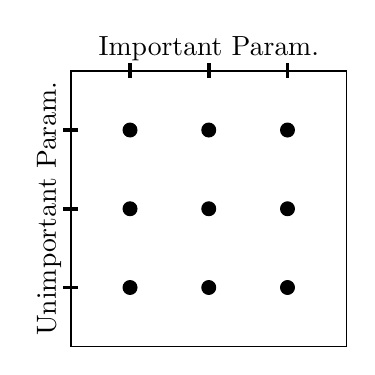
\begin{tikzpicture}[
									hp/.style = {
										draw,
										circle,
										fill = black,
										inner sep = 0,
										minimum width = 5pt,
										minimum height = 5pt
									},
									lv/.style = {
										draw,
										rectangle,
										fill = black,
										inner sep = 0,
										minimum width = 1pt,
										minimum height = 5pt
									},
									lh/.style = {
										draw,
										rectangle,
										fill = black,
										inner sep = 0,
										minimum width = 5pt,
										minimum height = 1pt
									}
								]
							\coordinate (a) at (-1.75, -1.75);
							\coordinate (b) at (+1.75, -1.75);
							\coordinate (c) at (+1.75, +1.75);
							\coordinate (d) at (-1.75, +1.75);

							\node [hp] at (-1, -1) {};
							\node [hp] at ( 0, -1) {};
							\node [hp] at (+1, -1) {};
							\node [hp] at (-1,  0) {};
							\node [hp] at ( 0,  0) {};
							\node [hp] at (+1,  0) {};
							\node [hp] at (-1, +1) {};
							\node [hp] at ( 0, +1) {};
							\node [hp] at (+1, +1) {};

							\node [lv] at (-1, +1.75) {};
							\node [lv] at ( 0, +1.75) {};
							\node [lv] at (+1, +1.75) {};

							\node [lh] at (-1.75, -1) {};
							\node [lh] at (-1.75,  0) {};
							\node [lh] at (-1.75, +1) {};

							\draw (a) -- (b) -- (c) -- (d) -- cycle;

							\path (c) -- node[above, sloped]{Important Param.} (d);
							\path (a) -- node[above, sloped]{Unimportant Param.} (d);
						\end{tikzpicture}
						\caption{Grid Search}
					\end{subfigure}
					~
					\begin{subfigure}{0.49\linewidth}
						\centering
						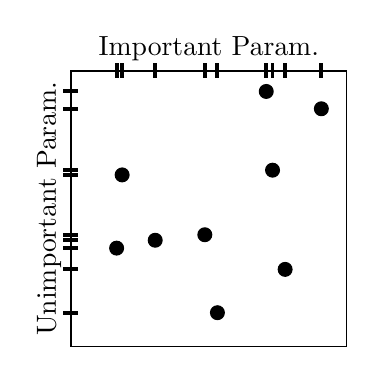
\begin{tikzpicture}[
									hp/.style = {
										draw,
										circle,
										fill = black,
										inner sep = 0,
										minimum width = 5pt,
										minimum height = 5pt
									},
									lv/.style = {
										draw,
										rectangle,
										fill = black,
										inner sep = 0,
										minimum width = 1pt,
										minimum height = 5pt
									},
									lh/.style = {
										draw,
										rectangle,
										fill = black,
										inner sep = 0,
										minimum width = 5pt,
										minimum height = 1pt
									}
								]
							\coordinate (a) at (-1.75, -1.75);
							\coordinate (b) at (+1.75, -1.75);
							\coordinate (c) at (+1.75, +1.75);
							\coordinate (d) at (-1.75, +1.75);

							\node [hp] at (+1.43, +1.27) {};
							\node [hp] at (+0.73, +1.49) {};
							\node [hp] at (+0.11, -1.32) {};
							\node [hp] at (-1.17, -0.50) {};
							\node [hp] at (-1.10, +0.43) {};
							\node [hp] at (+0.97, -0.77) {};
							\node [hp] at (-0.68, -0.40) {};
							\node [hp] at (+0.81, +0.49) {};
							\node [hp] at (-0.05, -0.33) {};

							\node [lv] at (+1.43, +1.75) {};
							\node [lv] at (+0.73, +1.75) {};
							\node [lv] at (+0.11, +1.75) {};
							\node [lv] at (-1.17, +1.75) {};
							\node [lv] at (-1.10, +1.75) {};
							\node [lv] at (+0.97, +1.75) {};
							\node [lv] at (-0.68, +1.75) {};
							\node [lv] at (+0.81, +1.75) {};
							\node [lv] at (-0.05, +1.75) {};

							\node [lh] at (-1.75, +1.27) {};
							\node [lh] at (-1.75, +1.49) {};
							\node [lh] at (-1.75, -1.32) {};
							\node [lh] at (-1.75, -0.50) {};
							\node [lh] at (-1.75, +0.43) {};
							\node [lh] at (-1.75, -0.77) {};
							\node [lh] at (-1.75, -0.40) {};
							\node [lh] at (-1.75, +0.49) {};
							\node [lh] at (-1.75, -0.33) {};

							\draw (a) -- (b) -- (c) -- (d) -- cycle;

							\path (c) -- node[above, sloped]{Important Param.} (d);
							\path (a) -- node[above, sloped]{Unimportant Param.} (d);
						\end{tikzpicture}
						\caption{Random Search}
					\end{subfigure}
					\caption{Comparison of grid search (left) and random search (right). It can be seen that for random search, more (nine) values of the important parameter are tried while when using grid search, only three values are tested.}
					\label{fig:gridRandomSearch}
				\end{figure}
			% end
		% end
	% end

	\section{Ensembles}
		\emph{Ensembles} leverage multiple simpler models for constructing a single big model with strong prediction power. There are two basic types for ensembles: \emph{Bagging} (Bootstrap Aggregation) and \emph{Boosting}. In bagging, multiple models are trained on samples of the data and a majority vote (for classification) or average (for regression) is used for prediction. In \emph{boosting}, the learners are ordered and training takes place one after another. Then each learner tries to reduce the residual error of the previous trainers on the examples that where misclassified. Bagging usually reduces the variance whereas boosting reduces the bias of the model (and also probably the variance, but this is not true for every model). In both cases, the resulting prediction is a sum or vote of the base learner predictions.

		Usually bagging yields around \SI{2}{\percent} of extra accuracy, so models can be made better but one can not fix a broken model using bagging. Hence, neural networks are fairly often used with bagging. But they are only rarely used with boosting. The reason for this is that deep neural networks usually model global effects and wide networks model local effects, whereas boosting models from global to local. This means that the first models of a boosting sequence models the global effects and later models are used for fine-tuning locally. So boosting with the same network architecture does not yield good results because the shift from global to local is not representable. An open questions is if it is possible to move from deep to wide networks the further the process of boosting gets. The problem that arises in this case is that it is hard to detect whether the next model in a boosting process models global or local properties.

		A common disadvantage of bagging and boosting is of course that it takes longer to train compared to a single model. One trick to circumvent this in bagging is to average multiple model checkpoints, i.e., the weights of a network at different iterations, rather than completely different models.
	% end

	\section{Dropout Regularization}
		As neural networks have lots of parameters, sometimes more than there is training data, overfitting is a big problem in deep learning. One regularization technique for tackling this is \emph{dropout}. The core concept of dropout is to randomly set some neurons to zero with probability \(p\) for each neuron during the forward pass, disabling them for the prediction. The idea is that this forces the network to learn redundant representations, making it more robust towards changes in the inputs. Another interpretation is that dropout trains a large ensemble of models that share parameters.

		During test time, it would be ideal to integrate out all the noise, but in practice this is obviously intractable. Instead, the result will be approximated using Monte Carlo integration techniques: calculate multiple forward passes using different (random) dropout masks and average all predictions. But in fact this can be done (approximately) with a single forward pass with all neurons being active! To compensate for the inflation caused by roughly \(1/p\) more neurons being active during the fully activated forward pass, all activations have to be scaled by \(p\).

		As scaling the activations at test time reveals details about the training process\footnote{Take, for example, a model that is deployed on lots on end-user devices (like a face detection model). If the developer finds a better way of training that improves the model, but uses dropout, the end-user model would have to be changed just because the training process changed.}, it is also possible to scale the activations by \(1/p\) in the training forward pass. This is called \emph{inverted dropout}.
	% end

	\section{Gradient Clipping}
		In gradient descent, big gradients cause divergence while small gradients cause slow convergence. As divergence is much worse and gradients can explode pretty fast, a technique called \emph{gradient clipping} can be used. Gradient clipping limits the magnitude of each gradient
		\begin{equation}
			\hat{g}_i = \min\big( g_\mathrm{max},\, \max(-g_\mathrm{max},\, g_i) \big)
		\end{equation}
		such that \( \lvert \hat{g}_i \rvert \leq g_\mathrm{max} \). Then a decreasing learning rate is used to converge to an optimum. Standard gradient clipping limits the larges gradient dimensions while others max be very small.

		An alternative, \emph{extreme} gradient clipping which is used in AdaGrad and RMSProp scale all dimensions by the inverse standard deviation such that all dimensions have unit standard deviation. An even more extreme approach are one-bit gradients where all gradient dimensions are clipped such that only their sign is left. This actually works on some problems! But usually, gradient clipping is not used this aggressive.
	% end

	\section{Gradient Noise}
		In stochastic gradient descent, the gradient resulting from the Monte Carlo approximations is noisy, but SGD still makes good progress on average. This gives the idea of whether it might be good to add a little noise to the gradients? Experiments have shown that this is actually the case, reducing overfitting in complex models. Usually the noise is additive
		\begin{equation}
			\hat{g}_i^{(k)} = g_i^{(k)} + \epsilon_t^{(k)},\quad \epsilon_t^{(k)} \sim \mathcal{N}(0, \sigma_k^2)
		\end{equation}
		with variance
		\begin{equation}
			\sigma_k^2 = \frac{\eta}{(1 + k) \gamma}
		\end{equation}
		where \( \eta \in \{ 0.01, 0.3, 1 \} \) and \( \gamma = 0.55 \). This way the noise added to the gradients is reduced over time, producing more stable gradients towards the end.

		Gradient noise raises some interesting theoretical questions as it turns the model parameters into a Bayesian inference task where the noise magnitude controls the temperature of the distribution (higher noise \(\to\) higher temperature). Cf. momentum which reduces the level of detail.
	% end

	\section{Vanishing Gradients and Residual Networks}
		The \emph{vanishing gradient problem} is like the opposite of exploding gradients: if an activation function like tanh is used which squashes all numbers between zero and one and only produces gradients between zero and one, multiplying many of these numbers together quickly approaches zero. As many activation values and activation function gradients are stacked on top of each other in a deep network, this causes the gradients to \emph{vanish} or \emph{die}. One way to circumvent this is to use \emph{residual networks} with add \emph{skip connections} from one layer to later layers (see \autoref{fig:resNet}).

		\begin{figure}
			\centering
			\begin{tikzpicture}[->]
				\node [neuron] (a) {};
				\node [neuron, right = 2 of a] (b) {};
				\node [neuron, right = 2 of b] (c) {};
				\node [neuron, right = 2 of c] (d) {};

				\draw (a) -> (b);
				\draw (b) -> (c);
				\draw (c) -> (d);

				\draw (a) to[bend left] (c);
				\draw (b) to[bend left] (d);
			\end{tikzpicture}
			\caption{Illustration of the skip connections in a residual network. To compute the gradient of a node with two outgoing connections, the two incoming gradients are added together. It is also possible to add connections that skip more than one layer.}
			\label{fig:resNet}
		\end{figure}
	% end
% end

\chapter{Convolutional Neural Networks}
	While fully connected neural networks (multilayer perceptrons) are extremely powerful, they are not really well suited for processing large images. This is due to the shear amount of parameters that would be needed for the first layers as all pixels are connected to every neuron. But images do not really have a global correlation, the spatial correlation is fairly local! Hence, fully connected layers are just a waste of resources. Instead, \emph{convolutional neural networks} (CNNs) use convolutions from computer vision as learnable filters to extract locally correlated information first and later plugging the downscaled result into fully connected layers for further processing.

	A convolution is described by an \( F_y \times F_x \) matrix that gets shifted along the input image using element-wise products and sums for computing a pixel at that point. \autoref{fig:convNoStrideNoPadding} illustrates this for a \(3 \times 3\) filter on a \(5 \times 5\) image. Obviously, the size of the image shrinks because the size of the filter. This can be circumvented by adding \emph{zero-padding}. This means that the edges of the image get extended by \( P_x \)/\( P_y \) zeros on all sides such that the image is bigger. It is also possible to specify a \emph{stride} \(S_x\)/\(S_y\) along the width/height which prescribes the number of pixels the filter is moved in every step. The default is a stride of one which is also used in \autoref{fig:convNoStrideNoPadding} (also referred to as "no stride"). Higher values for the stride result in a smaller output image.

	In real-world applications, input images may have multiple \emph{channels}. A channel is one layer of the image, e.g. the "red" layer in an RGB image. Usually images have three (RGB) or four (RGBA, with transparency) channels. Then a filter is created for each layer and the results of all these filters are added together after applying them. It is common to add a bias (which, for a single filter, is a scalar value) that gets added to each resulting pixel. Usually in CNNs multiple filters are used per layer in the network resulting in as many output channels as filters where used. So the filters do not interact within a layer, but the next layer can combine them as needed. A really good visualization of a filter processing an image is given here:
	\begin{center}
		\url{https://cs231n.github.io/assets/conv-demo/index.html}
	\end{center}

	Normally all parameters in a filter layer (weights and biases of the filters) are learnable, resulting in
	\begin{equation}
		\text{\#Parameters} = D \big( d F_x F_y + 1 \big)
	\end{equation}
	parameters where \(d\) is the number of input channels, \(D\) is the number of output channels, and \(F_x\)/\(F_y\) are the size of each filter (width/height). The \emph{activation volume} has the spatial size
	\begin{equation}
		O_{x/y} = \frac{I_{x/y} + 2 P_{x/y} - F_{x/y}}{S_{x/y}} + 1
	\end{equation}
	where \(O_{x/y}\) is the width/height of the output data, \(I_{x/y}\) is the width/height of the input data, \(P_{x/y}\) is the horizontal/vertical padding, and \(S_{x/y}\) is the horizontal/vertical stride. If square input data and filters are used, the equations simplify to
	\begin{align}
		\text{\#Parameters} &= D \big( d F^2 + 1 \big) &
		O &= \frac{I + 2 P - F}{S} + 1.
	\end{align}
	In convolutional networks, these kind of layers are then stacked on top of each other, forming a feature hierarchy (like in multilayer perceptrons). As usual, it is not good to shrink down the spatial dimensions too slow nor too fast. Common settings are power of two for the number of filters and filter sizes, padding and stride of \( (F, S, P) = (3, 1, 1) \), \( (F, S, P) = (5, 1, 2) \), \( (F, S, P) = (5, 2, ?) \)\footnote{Whatever fits for the padding.}, or \( (F, S, P) = (1, 1, 0) \). Usually the convolutional part of a network is followed by some fully connected layers for performing the actual classification/regression task. The interpretation is that the convolutional layers produce good features that can then be used by the following multiplayer perceptron.

	It is also perfectly fine to use a scalar filter which basically results in a dot product between the layer and the filters.

	% TODO: CNNs: Biology; 6.4, 6.5, 6.6, 6.7, 6.8, 6.9, 6.10, 6.11, 6.12, 6.13, 6.14, 6.15, 6.16, 6.17, 6.18, 6.19, 6.20, 6.21, 6.22, 6.23, 6.24, 6.25, 6.26, 6.27, 6.28, 6.123, 6.124, 6.125, 6.126

	\begin{figure}
		\centering
		\begin{tikzpicture}[yscale = -1]
			\begin{scope}[local bounding box = image]
				\draw (0, 0) grid (5, 5);
				\foreach [count = \i] \x in { 0, ..., 4 } {
					\foreach [count = \j] \y in { 0, ..., 4 } {
						\tikzmath{\val = int(sqrt(((\i - 3) * (\j - 3)) ^ 2));}
						\node at (\x + 0.5, \y + 0.5) {\(\val\)};
					}
				}
				\coordinate (a) at (1, 0);
				\coordinate (b) at (4, 0);
				\coordinate (c) at (4, 3);
				\coordinate (d) at (1, 3);
				\node at (1.8, 0.8) {\scriptsize \( \cdot 1 \)};
				\node at (2.8, 0.8) {\scriptsize \( \cdot 0 \)};
				\node at (3.8, 0.8) {\scriptsize \( \cdot 1 \)};
				\node at (1.8, 1.8) {\scriptsize \( \cdot 0 \)};
				\node at (2.8, 1.8) {\scriptsize \( \cdot 1 \)};
				\node at (3.8, 1.8) {\scriptsize \( \cdot 0 \)};
				\node at (1.8, 2.8) {\scriptsize \( \cdot 1 \)};
				\node at (2.8, 2.8) {\scriptsize \( \cdot 0 \)};
				\node at (3.8, 2.8) {\scriptsize \( \cdot 1 \)};
			\end{scope}

			\begin{scope}[local bounding box = convolution, shift = {($ (image.east) + (2cm, -1.5cm) $)}]
				\draw (0, 0) grid (3, 3);
				\node at (0 + 0.5, 0 + 0.5) {\(1\)};
				\node at (0 + 0.5, 1 + 0.5) {\(0\)};
				\node at (0 + 0.5, 2 + 0.5) {\(1\)};
				\node at (1 + 0.5, 0 + 0.5) {\(0\)};
				\node at (1 + 0.5, 1 + 0.5) {\(1\)};
				\node at (1 + 0.5, 2 + 0.5) {\(0\)};
				\node at (2 + 0.5, 0 + 0.5) {\(1\)};
				\node at (2 + 0.5, 1 + 0.5) {\(0\)};
				\node at (2 + 0.5, 2 + 0.5) {\(1\)};
			\end{scope}

			\begin{scope}[local bounding box = result, shift = {($ (convolution.east) + (2cm, -1.5cm) $)}]
				\draw (0, 0) grid (3, 3);
				\node at (0 + 0.5, 0 + 0.5) {\(5\)};
				\node at (0 + 0.5, 1 + 0.5) {\(4\)};
				\node at (0 + 0.5, 2 + 0.5) {\(5\)};
				\node at (1 + 0.5, 0 + 0.5) {\(4\)};
				\node at (1 + 0.5, 1 + 0.5) {\(4\)};
				\node at (1 + 0.5, 2 + 0.5) {\(4\)};
				\node at (2 + 0.5, 0 + 0.5) {\(5\)};
				\node at (2 + 0.5, 1 + 0.5) {\(4\)};
				\node at (2 + 0.5, 2 + 0.5) {\(5\)};
				\coordinate (A) at (1, 0);
				\coordinate (B) at (2, 0);
				\coordinate (C) at (2, 1);
				\coordinate (D) at (1, 1);
				\node at (1.225, 0.775) {\tiny \( \sum \)};
			\end{scope}

			\path (image) -- node{\(\ast\)} (convolution);
			\path (convolution) -- node{\(=\)} (result);

			\draw [line width = 2pt] (a) -- (b) -- (c) -- (d) -- cycle;
			\draw [line width = 2pt] (A) -- (B) -- (C) -- (D) -- cycle;
			\draw [line width = 1pt] (b) -- (convolution.north west);
			\draw [line width = 1pt] (c) -- (convolution.south west);
			\draw [line width = 1pt] (convolution.north east) -- (A);
			\draw [line width = 1pt] (convolution.south east) -- (D);
		\end{tikzpicture}
		\caption{Illustration of a \( 3 \times 3 \) convolution along an \( 5 \times 5 \) image.}
		\label{fig:convNoStrideNoPadding}
	\end{figure}

	\section{Pooling}
		A \emph{pooling} layer scales the input down by combining multiple pixels into a single pixel (like a convolution), but usually destructive operations like a maximum (known as \emph{max pooling}) are used. In contrast to convolutional layers, pooling layers operate independently on the input channels, producing as many output channels as there are input channels (i.e., the results to not get combined).
	% end

	\section{Case Studies}
		This section covers some case studies (concrete models) used for certain tasks, usually classification.

		Like previously for multi-layer perceptrons, the trend goes toward using smaller filters and instead using deeper architectures. Another trend is to get rid of pooling and fully connected layers and instead just use convolutional layers.

		\paragraph{LeNet-5}
			LeNet-5 was proposed by LeCun et al. in 1998 for classification on the MNIST dataset:
			\begin{enumerate}
				\item Convolution, \num{6} filters, size \(5 \times 5\), stride \num{1}, pad \num{2}.
				\item Max pooling, size \(2 \times 2\), stride \num{2}.
				\item Convolution, \num{16} filters, size \(5 \times 5\), stride \num{1}, pad \num{0}.
				\item Max pooling, size \(2 \times 2\), stride \num{2}.
				\item Fully connected, \num{120} neurons.
				\item Fully connected, \num{84} neurons.
				\item Fully connected (output), \num{10} neurons.
			\end{enumerate}
		% end

		\paragraph{AlexNet}
			AlexNet was proposed by Krizhevsky et al. in 2012 and is more advanced and evolved than LeNet-5:
			\begin{enumerate}
				\item Convolution, \num{96} filters, size \( 11 \times 11 \), stride \num{4}, pad \num{0}.
				\item Max pooling, size \(3 \times 3\), stride \num{2}.
				\item Normalization.
				\item Convolution, \num{256} filters, site \(5 \times 5\), stride \num{1}, pad \num{2}.
				\item Max pooling, size \(3 \times 3\), stride \num{2}.
				\item Normalization.
				\item Convolution, \num{384} filters, size \(3 \times 3\), stride \num{1}, pad \num{1}.
				\item Convolution, \num{384} filters, size \(3 \times 3\), stride \num{1}, pad \num{1}.
				\item Convolution, \num{256} filters, size \(3 \times 3\), stride \num{1}, pad \num{1}.
				\item Max pooling, size \(3 \times 3\), stride \num{2}.
				\item Fully connected, \num{4096} neurons.
				\item Fully connected, \num{4096} neurons.
				\item Fully connected, \num{1000} neurons.
			\end{enumerate}
			Further details: AlexNet was the first model to use ReLU activations and used normalization layers which is not common anymore. Furthermore heavy data augmentation was done as well as dropout with \(p = 0.5\).
		% end
	% end

	\section{Transfer Learning}
		A common saying about CNNs and computer vision tasks in general is that they take a lot of data for training. While is is true for training untrained models, it is possible to use pre-trained models and fine-tune them on the data at hand. This is called \emph{transfer learning}. The idea is to take a trained deep CNN that was, for example, trained on ImageNet and plug an untrained \emph{classification head}, fix all weights of the "body" of the model and only train the weights and biases of the head. This way deep features provided by the pre-trained model can be used as these are utterly effective, but training time and the amount of data needed is still relatively low. If more data is available, it might also be possible to fine-tune some of the convolutional layers for even better accuracy, but this is often not even needed. Tip: use a smaller learning rate for fine-tuning the final layers (around \(1/10\) of the original learning rate) and use even smaller rates for intermediate layers (around \(1/100\) of the original learning rate).
	% end
% end

\chapter{Computer Vision Tasks}
	This chapter covers tasks that are common in computer vision like classification, localization, and object detection. In classification, the task is to classify a given image based on what is in it. In combined classification and localization, the image is classified and a bounding box is detected around the object that was classified. Object detection describes the same but for multiple objects, so multiple different objects can be classified and localized within an image. In \emph{image segmentation}, the bounding box is extended so a polygon that gets built around the objects. This is the hardest task of the four. \autoref{fig:computerVisionTasks} shows a comparison of the four tasks.

	\begin{figure}
		\centering
		\begin{subfigure}{0.24\linewidth}
			\captionsetup{justification=centering}
			\centering
			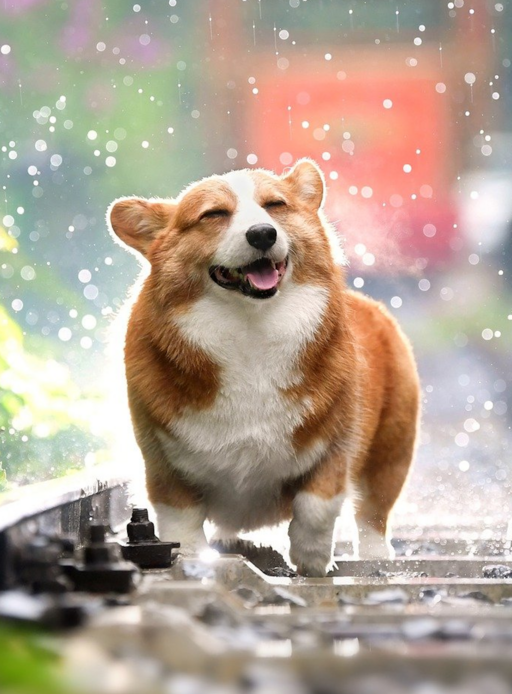
\includegraphics[width=\linewidth]{img/compressed-dog.png}
			\caption{Classification \\ Dog}
		\end{subfigure}
		\begin{subfigure}{0.24\linewidth}
			\captionsetup{justification=centering}
			\centering
			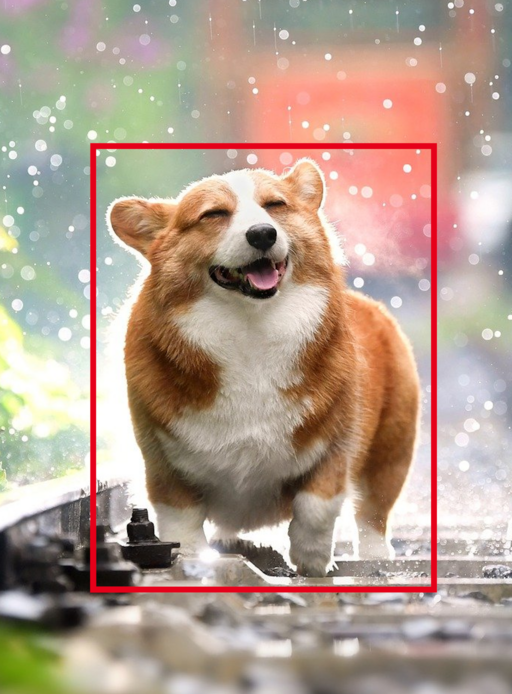
\includegraphics[width=\linewidth]{img/compressed-dog-localized.png}
			\caption{Class. \& Localization \\ Dog}
		\end{subfigure}
		\begin{subfigure}{0.24\linewidth}
			\captionsetup{justification=centering}
			\centering
			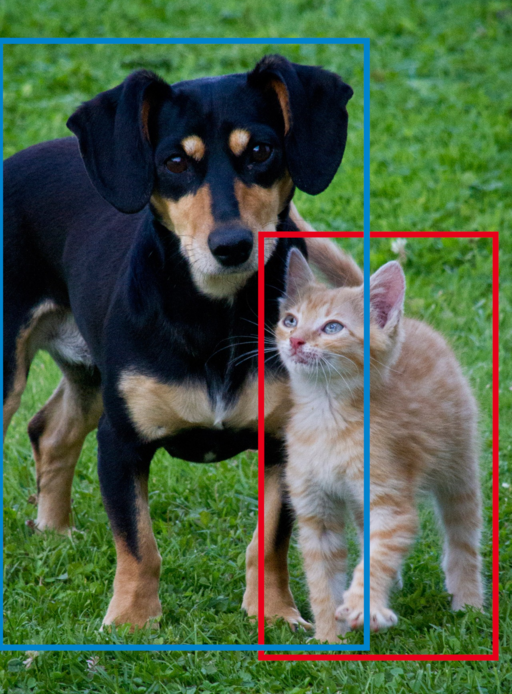
\includegraphics[width=\linewidth]{img/compressed-dog-and-cat-detected.png}
			\caption{Object Detection \\ {\color{TUDa-2b} Dog}, {\color{TUDa-9b} Cat}}
		\end{subfigure}
		\begin{subfigure}{0.24\linewidth}
			\captionsetup{justification=centering}
			\centering
			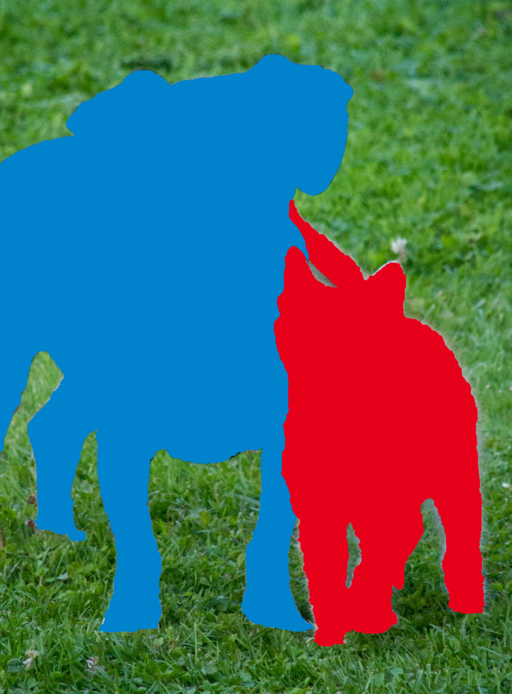
\includegraphics[width=\linewidth]{img/compressed-dog-and-cat-segmented.png}
			\caption{Object Segmentation \\ {\color{TUDa-2b} Dog}, {\color{TUDa-9b} Cat}}
		\end{subfigure}
		\caption{Comparison of computer vision task, from the easiest (left) to the hardest (right).}
		\label{fig:computerVisionTasks}
	\end{figure}

	\section{Combined Classification and Localization}
		In classification, the input to the model is an image and the output is a class label. In localization, the input to the model is an image and the output is a box in the image, given by its coordinates and its width/height.

		Interpreting localization as regression is a pretty natural thing to do as the output is (kind of) continuous. For training such a model, a cross-entropy loss is used for classification and an L2 loss is used for regression separately. The process is as follows: firstly, train or download a classification model. Secondly, attach a new regression head to the network that will be used for localization. The network is now two-headed. Then fix the downloaded CNN and train only the regression head using the L2 loss and after that potentially fine-tune the classification head. At test time, both heads are used simultaneously to retrieve both class scores and box coordinates.

		For localizing multiple objects in an image (e.g. whole face, left ear, right ear, etc.), the regression head can also output \( 4K \) numbers where \(K\) is the number of objects to localize. Compared to object detection, the number of objects that are detected is fixed and there is only one class label for the image. One application is for example human pose estimation where the \(K\) objects represent the \(K\) joints of a human.

		To further optimize the accuracy of the predictions a \emph{sliding window} can be used that slides over the input image and executes the classification and regression network multiple times. The predictions are then combined into a single final prediction. One example model that uses this technique is Overfeat which uses many sliding window locations and multiple scales. Also, the fully connected layers are turned into convolutions for more efficiency.
	% end

	\section{Object Detection}
		Compared to combined classification and localization, in object detection a variable sized output is necessary. One approach is again using a sliding window which has the disadvantage that the classifier has to be executed lots of times. But if the model is sufficiently fast, this is a good approach. Additionally it is possible to only look at a tiny subset of possible positions using \emph{region proposals}. Region proposals first find "blobby" image regions which probably contain objects and then a classification model is applied to these proposals for detecting objects. This massively reduces the amount of regions that need to be scanned such that powerful, yet resource hungry, models like CNNs can be used. This then forms the \emph{R-CNN} model.

		But in the end, all approaches discussed here are really the human way. One thing is that given an image and a classification task, humans often do not detect objects which are far larger than usual, but deep CNNs do\footnote{Miguel P. Eckstein, Kathryn Koehler, Lauren E. Welbourne, and Emre Akbas (2017): "Humans, but Not Deep Neural Networks, Often Miss Giant Targets in Scenes"}.

		% TODO: Object Detection: Histogram of Oriented Gradients, Deformable Parts Model; 7.73, 7.74, 7.75

		\subsection{R-CNN}
			\emph{R-CNN} combines regions proposals with CNNs to form an efficient detector. For training R-CNNs, the process is as follows:
			\begin{enumerate}
				\item Train or download a classification model for ImageNet (e.g. AlexNet).
				\item Reinitialize and fine-tune the final fully connected layer on a small portion of the classes that should be detected.
				\item Extract training features by extracting the region proposals and cropping/scaling them such that they fit into the CNN. Then save all outputs of the final pooling layer.
				\item Train a binary support vector machine per class to classify the features extracted in the previous step.
				\item Train a linear regression model per class to map from the images to offsets of the bounding box. This makes up for region proposals that where slightly wrong (too wide, small, etc.).
			\end{enumerate}
			To evaluate the performance of R-CNNs, the \emph{mean average precision} (mAP) is used: compute the \emph{average precision} (AP) separately for each class and then average over the classes. It is computed as follows. A detection is a true positive if the intersection over union with the true box is greater than some threshold (usually \num{0.5}). Then to compute the AP all detections are used to draw a precision/recall-curve. The AP then is the area under the curve.

			Problems of R-CNN is that it is slow at test time as a full forward pass through the CNN has to be computed for each region proposals. Also the SVMs and regressors are post-hoc, i.e., the CNN features are not updated in response to the SVMs and regressors. And the training process is really complicated.

			\subsubsection{Fast R-CNN}
				\emph{Fast R-CNN} is a variant of R-CNN that speeds up predictions at test time by sharing computation of convolutional layers between proposals for an image. Also, to tackle the second and third problem of R-CNNs, the whole model is just trained end-to-end with no complex training pipeline. Compared to vanilla R-CNN, Fast R-CNN is \num{25} times faster at test time.
			% end

			\subsubsection{Faster R-CNN}
				An even faster version of R-CNN is \emph{Faster R-CNN} where the extraction of regional proposals is done after the convolutional layers using a \emph{region proposal network} (RPN). This works by sliding a small window along the feature map that uses a small network that is used to classify between "object" and "not object" and outputs bounding boxes (which are used for finer localization in reference to the current window).

				To train Faster R-CNN, the original paper proposed an ugly pipeline consisting of alternating optimization of the RPN and all other components. But since then, the community shifted to just training everything jointly using four losses: RPN classification, RPN regression, Fast R-CNN classification, and Fast R-CNN regression. Compared to vanilla R-CNN, Faster R-CNN is \num{250} times faster at test time.
			% end
		% end

		\subsection{YOLO: You Only Look Once}
			The \emph{You Only Look Once} (YOLO) model uses a different approach than R-CNN and interprets object detection as regression. The image is divided into an \(S \times S\) grid and within each cell bounding boxes with four coordinated and their respective confidence as well as \(C\) class scores are calculated. The model than directly predicts these values using a CNN onto a \( 7 \times 7 \times (5 \cdot B + C) \) tensor. The YOLO model is even faster than Faster R-CNN, but the prediction power is not as good.
		% end
	% end
% end

\chapter{Recurrent Neural Networks}
	Until now, all discussed neural networks all have a clear topological ordering and a sensor of forward and backward and they can only process one input at a time, producing a single output. \emph{Recurrent neural networks} (RNNs) are a generalization of so-called \emph{feedforward networks} to networks that have a notion of "time" by introducing cycles. They are designed for processing a sequence \( \dotsrange{\vec{x}_1}{\vec{x}_n} \) of inputs and producing a sequence \( \dotsrange{\vec{y}_1}{\vec{y}_m} \) of outputs. \autoref{fig:rnnCell} shows a single RNN cell with its hidden state \(\vec{h}_t\) and how it processes a single input \(\vec{x}_t\). The computed hidden state is then stored and used for the next incoming vector.

	To compute a forward- and backward-pass (i.e., computing the gradients), RNNs are usually unrolled in time, forming a computational graph that can be differentiated. \autoref{fig:rnnCellUnrolled} illustrates the unrolling for three time steps and a single RNN cell. It is also often done to stack multiple RNN layers on top of each other, i.e., multiple RNN cells, each with an own hidden state, computed after each other. This is shown in \autoref{fig:rnnMultipleCellsUnrolled} for two cells and again three time steps. The nodes on the same level share all parameters while the nodes behind each other (producing the two separate hidden states) do not share weights.

	In general, the RNN formalism is extremely powerful and offers lots of flexibility. As it is a complete generalization of feedforward neural networks, they would theoretically also allow a one-to-one mapping, but this is usually not called an RNN. But they allow also for lots of other mapping types:
	\begin{description}[leftmargin = 3cm]
		\item[One-to-One]   This is equivalent to a vanilla neural network. A single input is mapped onto a single output. An example application is image classification.
		\item[One-to-Many]  A single input is mapped onto multiple outputs. An example application is image captioning where the RNN gets features extracted by a CNN and generated a sequence of words that describe the image.
		\item[Many-to-One]  Multiple inputs are mapped onto a single output. An example application is sentiment classification where a sequence of words is read and the RNN predicts the sentiment of the sentence (e.g. positive/negative).
		\item[Many-to-Many] Multiple inputs are mapped onto multiple outputs. This mode can come in two variants: either an output for time \(t\) is generated directly after reading the input at time \(t\) or all outputs are generated after the last item has been read. Of course various mixtures and different delays may also be used. Example applications are model learning where the RNN learns to predict the next position/velocity of e.g. a pendulum (first variant) and machine translation (second variant).
	\end{description}
	These four/five variants are illustrated in \autoref{fig:rnnVariants}.

	\begin{figure}
		\centering
		\begin{tikzpicture}[->]
			\node [draw, rectangle, minimum width = 1cm, minimum height = 1cm, inner sep = 0] (b) {};
			\coordinate [above = 0.25cm of b.west] (A1);
			\coordinate [below = 0.25cm of b.west] (A2);
			\coordinate [above = 0.25cm of b.east] (B1);
			\coordinate [below = 0.25cm of b.east] (B2);
			\node [left  = 1.5 of A1] (a) {\( \vec{x}_t \)};
			\node [right = 1.5 of B1] (c) {\( \vec{y}_t \)};

			\coordinate [right = 0.50 of B2] (n1);
			\coordinate [below = 0.75 of n1] (n2);
			\coordinate [left  = 0.50 of A2] (n4);
			\coordinate [below = 0.75 of n4] (n3);

			\draw (a) to (A1);
			\draw (B1) to (c);
			\draw [dashed] (B2) to (n1) to node[right]{\( \vec{h}_t \)} (n2) to (n3) to node[left]{\( \vec{h}_{t - 1} \)} (n4) to (A2);
		\end{tikzpicture}
		\caption{Illustration of a single RNN cell processing an input \(\vec{x}_t\), producing an output \(\vec{y}_t\) and a hidden state \(\vec{h}_t\) that is delayed one time step.}
		\label{fig:rnnCell}
	\end{figure}

	\begin{figure}
		\centering
		\begin{subfigure}{0.49\linewidth}
			\centering
			\begin{tikzpicture}[->]
				\node [draw, rectangle, minimum width = 1cm, minimum height = 1cm, inner sep = 0] (a1) {};
				\coordinate [below = 0.25cm of a1.west] (a1L);
				\coordinate [below = 0.25cm of a1.east] (a1R);
				\node [left  = 1.5 of a1, yshift = -0.25cm] (a1x) {\( \vec{x}_0 \)};
				\node [right = 1.5 of a1, yshift = +0.25cm] (a1y) {\( \vec{y}_0 \)};

				\node [draw, rectangle, minimum width = 1cm, minimum height = 1cm, inner sep = 0, below = 1 of a1] (a2) {};
				\coordinate [below = 0.25cm of a2.west] (a2L);
				\coordinate [below = 0.25cm of a2.east] (a2R);
				\node [left  = 1.5 of a2, yshift = -0.25cm] (a2x) {\( \vec{x}_1 \)};
				\node [right = 1.5 of a2, yshift = +0.25cm] (a2y) {\( \vec{y}_1 \)};

				\node [draw, rectangle, minimum width = 1cm, minimum height = 1cm, inner sep = 0, below = 1 of a2] (a3) {};
				\coordinate [below = 0.25cm of a3.west] (a3L);
				\coordinate [below = 0.25cm of a3.east] (a3R);
				\node [left  = 1.5 of a3, yshift = -0.25cm] (a3x) {\( \vec{x}_2 \)};
				\node [right = 1.5 of a3, yshift = +0.25cm] (a3y) {\( \vec{y}_2 \)};

				\path (a1) to coordinate(A) (a2);
				\path (a2) to coordinate(B) (a3);
				\coordinate [below = 0.5 of a3] (C);

				\draw (a1x) to ($ (a1.west) + (0, -0.25) $);
				\draw ($ (a1.east) + (0, +0.25) $) to (a1y);
				\draw (a2x) to ($ (a2.west) + (0, -0.25) $);
				\draw ($ (a2.east) + (0, +0.25) $) to (a2y);
				\draw (a3x) to ($ (a3.west) + (0, -0.25) $);
				\draw ($ (a3.east) + (0, +0.25) $) to (a3y);

				\draw ($ (a1.east) + (0, -0.25) $) to ($ (a1.east) + (0.5, -0.25) $) |- node[right, pos = 0.05]{\( \vec{h}_0 \)} (A) -| ($ (a2.west) + (-0.5, +0.25) $) to ($ (a2.west) + (0, +0.25) $);
				\draw ($ (a2.east) + (0, -0.25) $) to ($ (a2.east) + (0.5, -0.25) $) |- node[right, pos = 0.05]{\( \vec{h}_1 \)} (B) -| ($ (a3.west) + (-0.5, +0.25) $) to ($ (a3.west) + (0, +0.25) $);
				\draw ($ (a3.east) + (0, -0.25) $) to ($ (a3.east) + (0.5, -0.25) $) |- node[right, pos = 0.05]{\( \vec{h}_2 \)} (C) -| ($ (C) + (-1, -0.5) $);
			\end{tikzpicture}
			\caption{Unrolling with analogous notation to \autoref{fig:rnnCell}.}
		\end{subfigure}
		~
		\begin{subfigure}{0.49\linewidth}
			\centering
			\begin{tikzpicture}[->]
				\node [draw, rectangle, minimum width = 1cm, minimum height = 1cm, inner sep = 0] (a1) {};
				\node [draw, rectangle, minimum width = 1cm, minimum height = 1cm, inner sep = 0, right = 1 of a1] (a2) {};
				\node [draw, rectangle, minimum width = 1cm, minimum height = 1cm, inner sep = 0, right = 1 of a2] (a3) {};
				\coordinate [right = 1 of a3] (a4);

				\node [below = 1 of a1] (a1x) {\( \vec{x}_0 \)};
				\node [below = 1 of a2] (a2x) {\( \vec{x}_1 \)};
				\node [below = 1 of a3] (a3x) {\( \vec{x}_2 \)};

				\node [above = 1 of a1] (a1y) {\( \vec{y}_0 \)};
				\node [above = 1 of a2] (a2y) {\( \vec{y}_1 \)};
				\node [above = 1 of a3] (a3y) {\( \vec{y}_2 \)};

				\draw (a1x) to (a1);
				\draw (a2x) to (a2);
				\draw (a3x) to (a3);
				\draw (a1) to (a1y);
				\draw (a2) to (a2y);
				\draw (a3) to (a3y);

				\draw (a1) to node[above]{\( \vec{h}_0 \)} (a2);
				\draw (a2) to node[above]{\( \vec{h}_1 \)} (a3);
				\draw (a3) to node[above]{\( \vec{h}_2 \)} (a4);
			\end{tikzpicture}
			\caption{Unrolling how it is usually drawn.}
		\end{subfigure}
		\caption{First three node of an unrolled recurrent neural network with the hidden state \(\vec{h}_t\). The two pictures show the same model using two different notations.}
		\label{fig:rnnCellUnrolled}
	\end{figure}

	\begin{figure}
		\centering
		\begin{tikzpicture}[->]
			\node [draw, rectangle, minimum width = 1cm, minimum height = 1cm, inner sep = 0] (a1) {};
			\node [draw, rectangle, minimum width = 1cm, minimum height = 1cm, inner sep = 0, right = 1 of a1] (a2) {};
			\node [draw, rectangle, minimum width = 1cm, minimum height = 1cm, inner sep = 0, right = 1 of a2] (a3) {};
			\coordinate [right = 1 of a3] (a4);

			\node [draw, rectangle, minimum width = 1cm, minimum height = 1cm, inner sep = 0, above = 1 of a1] (b1) {};
			\node [draw, rectangle, minimum width = 1cm, minimum height = 1cm, inner sep = 0, right = 1 of b1] (b2) {};
			\node [draw, rectangle, minimum width = 1cm, minimum height = 1cm, inner sep = 0, right = 1 of b2] (b3) {};
			\coordinate [right = 1 of b3] (b4);

			\node [below = 1 of a1] (x1) {\( \vec{x}_0 \)};
			\node [below = 1 of a2] (x2) {\( \vec{x}_1 \)};
			\node [below = 1 of a3] (x3) {\( \vec{x}_2 \)};

			\node [above = 1 of b1] (y1) {\( \vec{y}_{10} \)};
			\node [above = 1 of b2] (y2) {\( \vec{y}_{11} \)};
			\node [above = 1 of b3] (y3) {\( \vec{y}_{12} \)};

			\draw (x1) to (a1);
			\draw (x2) to (a2);
			\draw (x3) to (a3);
			\draw (a1) to node[left, near start]{\( \vec{x}_{00} \)} node[right, near end]{\( \vec{y}_{00} \)} (b1);
			\draw (a2) to node[left, near start]{\( \vec{x}_{01} \)} node[right, near end]{\( \vec{y}_{01} \)} (b2);
			\draw (a3) to node[left, near start]{\( \vec{x}_{02} \)} node[right, near end]{\( \vec{y}_{02} \)} (b3);
			\draw (b1) to (y1);
			\draw (b2) to (y2);
			\draw (b3) to (y3);

			\draw (a1) to node[above]{\( \vec{h}_{00} \)} (a2);
			\draw (a2) to node[above]{\( \vec{h}_{01} \)} (a3);
			\draw (a3) to node[above]{\( \vec{h}_{02} \)} (a4);
			\draw (b1) to node[above]{\( \vec{h}_{10} \)} (b2);
			\draw (b2) to node[above]{\( \vec{h}_{11} \)} (b3);
			\draw (b3) to node[above]{\( \vec{h}_{12} \)} (b4);
		\end{tikzpicture}
		\caption{RNN with two RNN cells after each other. This picture shows the unrolled RNN for three time steps.}
		\label{fig:rnnMultipleCellsUnrolled}
	\end{figure}

	\begin{figure}
		\centering
		\begin{subfigure}{0.135\linewidth}
			\centering
			\begin{tikzpicture}[->, every node/.style = { draw, rectangle, minimum width = 0.5cm, minimum height = 1cm, inner sep = 0 }, input/.style = { fill = TUDa-9a }, hidden/.style = { fill = TUDa-4a }, output/.style = { fill = TUDa-2a }]
				\node [input] (a1) {};
				\node [hidden, above = 1 of a1] (b1) {};
				\node [output, above = 1 of b1] (c1) {};
				\draw (a1) to (b1);
				\draw (b1) to (c1);
			\end{tikzpicture}
			\caption{One-to-One}
		\end{subfigure}
		~
		\begin{subfigure}{0.167\linewidth}
			\centering
			\begin{tikzpicture}[->, every node/.style = { draw, rectangle, minimum width = 0.5cm, minimum height = 1cm, inner sep = 0 }, input/.style = { fill = TUDa-9a }, hidden/.style = { fill = TUDa-4a }, output/.style = { fill = TUDa-2a }]
				\node [input] (a1) {};
				\node [hidden, above = 1   of a1] (b1) {};
				\node [hidden, right = 0.5 of b1] (b2) {};
				\node [hidden, right = 0.5 of b2] (b3) {};
				\node [output, above = 1   of b1] (c1) {};
				\node [output, above = 1   of b2] (c2) {};
				\node [output, above = 1   of b3] (c3) {};
				\draw (a1) to (b1);
				\draw (b1) to (b2);
				\draw (b2) to (b3);
				\draw (b1) to (c1);
				\draw (b2) to (c2);
				\draw (b3) to (c3);
			\end{tikzpicture}
			\caption{One-to-Many}
		\end{subfigure}
		~
		\begin{subfigure}{0.167\linewidth}
			\centering
			\begin{tikzpicture}[->, every node/.style = { draw, rectangle, minimum width = 0.5cm, minimum height = 1cm, inner sep = 0 }, input/.style = { fill = TUDa-9a }, hidden/.style = { fill = TUDa-4a }, output/.style = { fill = TUDa-2a }]
				\node [input] (a1) {};
				\node [input, right = 0.5 of a1] (a2) {};
				\node [input, right = 0.5 of a2] (a3) {};
				\node [hidden, above = 1 of a1] (b1) {};
				\node [hidden, above = 1 of a2] (b2) {};
				\node [hidden, above = 1 of a3] (b3) {};
				\node [output, above = 1 of b3] (c3) {};
				\draw (a1) to (b1);
				\draw (a2) to (b2);
				\draw (a3) to (b3);
				\draw (b1) to (b2);
				\draw (b2) to (b3);
				\draw (b3) to (c3);
			\end{tikzpicture}
			\caption{Many-to-One}
		\end{subfigure}
		~
		\begin{subfigure}{0.167\linewidth}
			\centering
			\begin{tikzpicture}[->, every node/.style = { draw, rectangle, minimum width = 0.5cm, minimum height = 1cm, inner sep = 0 }, input/.style = { fill = TUDa-9a }, hidden/.style = { fill = TUDa-4a }, output/.style = { fill = TUDa-2a }]
				\node [input] (a1) {};
				\node [input, right = 0.5 of a1] (a2) {};
				\node [input, right = 0.5 of a2] (a3) {};
				\node [hidden, above = 1 of a1] (b1) {};
				\node [hidden, above = 1 of a2] (b2) {};
				\node [hidden, above = 1 of a3] (b3) {};
				\node [output, above = 1 of b1] (c1) {};
				\node [output, above = 1 of b2] (c2) {};
				\node [output, above = 1 of b3] (c3) {};
				\draw (a1) to (b1);
				\draw (a2) to (b2);
				\draw (a3) to (b3);
				\draw (b1) to (b2);
				\draw (b2) to (b3);
				\draw (b1) to (c1);
				\draw (b2) to (c2);
				\draw (b3) to (c3);
			\end{tikzpicture}
			\caption{Many-to-Many}
		\end{subfigure}
		~
		\begin{subfigure}{0.28\linewidth}
			\centering
			\begin{tikzpicture}[->, every node/.style = { draw, rectangle, minimum width = 0.5cm, minimum height = 1cm, inner sep = 0 }, input/.style = { fill = TUDa-9a }, hidden/.style = { fill = TUDa-4a }, output/.style = { fill = TUDa-2a }]
				\node [input] (a1) {};
				\node [input, right = 0.5 of a1] (a2) {};
				\node [input, right = 0.5 of a2] (a3) {};
				\node [hidden, above = 1 of a1] (b1) {};
				\node [hidden, above = 1 of a2] (b2) {};
				\node [hidden, above = 1 of a3] (b3) {};
				\node [hidden, right = 0.5 of b3] (b4) {};
				\node [hidden, right = 0.5 of b4] (b5) {};
				\node [output, above = 1 of b3] (c3) {};
				\node [output, above = 1 of b4] (c4) {};
				\node [output, above = 1 of b5] (c5) {};
				\draw (a1) to (b1);
				\draw (a2) to (b2);
				\draw (a3) to (b3);
				\draw (b1) to (b2);
				\draw (b2) to (b3);
				\draw (b3) to (b4);
				\draw (b4) to (b5);
				\draw (b3) to (c3);
				\draw (b4) to (c4);
				\draw (b5) to (c5);
			\end{tikzpicture}
			\caption{Many-to-Many}
		\end{subfigure}
		\caption{Illustration of the four/five variants of RNN applications.}
		\label{fig:rnnVariants}
	\end{figure}

	\section{Vanilla RNN}
		The dynamics of the hidden state of a vanilla RNN as illustrated in \autoref{fig:rnnCell} is described by a parametric function
		\begin{equation}
			\vec{h}_t = \vec{f}_{\vec{\theta}}(\vec{h}_{t - 1}, \vec{x}_t)
		\end{equation}
		where \( \vec{h}_t \) and \( \vec{h}_{t - 1} \) are the next and current time step, respectively, and \(\vec{x}_t\) is the current input. This formula is then iterated for every step of the input sequence (with the same function and parameters per step). Usually the function \( \vec{f}_{\vec{\theta}} \) is a tanh with linear combinations of the hidden state and input as parameters
		\begin{equation}
			\vec{f}_{\vec{\theta}} = \tanh\!\big( \mat{W}_{hh} \vec{h}_{t - 1} + \mat{W}_{xh} \vec{x}_t \big)  \label{eq:rnnHidden}
		\end{equation}
		with \( \vec{\theta} = \big\{ \mat{W}_{hh}, \mat{W}_{xh} \big\} \). The hidden state is then re-weighted, forming the output of the RNN cell:
		\begin{equation}
			\vec{y}_t = \mat{W}_{hy} \vec{h}_t
		\end{equation}
		This can either be taken as the output or be fed into another neural network, often a fully connected one. For one-to-many and delayed many-to-many RNNs, the inputs of the cells that do not have inputs are just set to zero such that they are ignored in \autoref{eq:rnnHidden}.

		% TODO: Vanilla RNN: Interpretable Cells; 8.62, 8.63, 8.64, 8.65, 8.66, 8.67

		\subsection{Image Captioning}
			For using RNNs in image captioning, the hidden state is usually high-dimensional and \(\vec{h}_0\) is initialized with the output of a CNN. Then a "start" token is fed into the RNN as the first input and the second input is just the first output. To indicate that the captioning is complete the RNN spits out an "end" token. This is illustrated in \autoref{fig:rnnImageCaptioning}. Instead of initializing \(\vec{h}_0\) it may also be helpful to learn an additional matrix that transforms the first input
			\begin{equation}
				\vec{f}_{\vec{\theta}} = \tanh\!\big( \mat{W}_{hh} \vec{h}_{t - 1} + \mat{W}_{xh} \vec{x}_t + \mat{W}_{ih} \vec{v} \big),
			\end{equation}
			where \( \vec{v} \) is the output vector of the CNN. Fancier models for image captioning use \emph{attention} to look at different parts of the image for different parts of the caption. This is covered in more detail in \autoref{c:attention}.

			\begin{figure}
				\centering
				\begin{tikzpicture}[->, label distance = -5pt, every node/.style = { draw, rectangle, minimum width = 0.5cm, minimum height = 1cm, inner sep = 0 }, input/.style = { fill = TUDa-9a }, hidden/.style = { fill = TUDa-4a }, output/.style = { fill = TUDa-2a }]
					\node [inner sep = 2pt] (image) {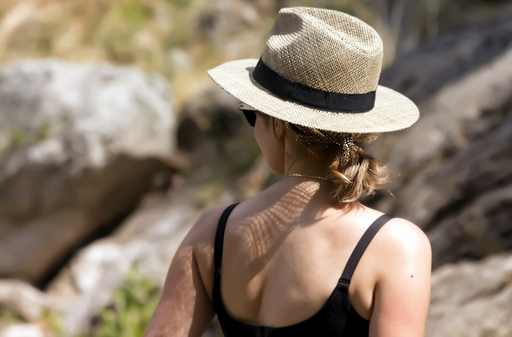
\includegraphics[width = 4cm]{img/compressed-straw-hat.png}};
					\node [draw, rectangle, right = 1.5 of image, minimum width = 1.5cm] (cnn) {CNN};
					\node [hidden, right = 1.5 of cnn] (b1) {};
					\node [hidden, right = 1.25 of b1] (b2) {};
					\node [hidden, right = 1.25 of b2] (b3) {};
					\node [hidden, right = 1.25 of b3] (b4) {};
					\node [hidden, right = 1.25 of b4] (b5) {};
					\node [input, below = 1 of b1, label = below:{START}] (a1) {};
					\node [input, below = 1 of b2, label = below:{"woman"}] (a2) {};
					\node [input, below = 1 of b3, label = below:{"with"}] (a3) {};
					\node [input, below = 1 of b4, label = below:{"straw"}] (a4) {};
					\node [input, below = 1 of b5, label = below:{"hat"}] (a5) {};
					\node [output, above = 1 of b1, label = above:{"woman"}] (c1) {};
					\node [output, above = 1 of b2, label = above:{"with"}] (c2) {};
					\node [output, above = 1 of b3, label = above:{"straw"}] (c3) {};
					\node [output, above = 1 of b4, label = above:{"hat"}] (c4) {};
					\node [output, above = 1 of b5, label = above:{END}] (c5) {};

					\draw (image) to (cnn);
					\draw (cnn) to (b1);
					\draw (b1) to (b2);
					\draw (b2) to (b3);
					\draw (b3) to (b4);
					\draw (b4) to (b5);
					\draw (a1) to (b1);
					\draw (a2) to (b2);
					\draw (a3) to (b3);
					\draw (a4) to (b4);
					\draw (a5) to (b5);
					\draw (b1) to (c1);
					\draw (b2) to (c2);
					\draw (b3) to (c3);
					\draw (b4) to (c4);
					\draw (b5) to (c5);
				\end{tikzpicture}
				\caption{Illustration of image captioning using a CNN to initialize the hidden state.}
				\label{fig:rnnImageCaptioning}
			\end{figure}
		% end
	% end

	\section{Long Short-Term Memory (LSTM)}
		One problem with vanilla RNNs is that if the sequences are very long, gradients vanish quickly as the tangent always reduces the gradient values. Also, if the largest Eigenvalue of weight matrix for the hidden state is larger than one, gradient will explode. If it is lower than one, they will vanish. So only for a single Eigenvalue the gradients are stable. \emph{Long short-term memory networks} tackle the problem of vanishing gradients by adding "highway"\footnote{Not to be confused with highway networks!} connections for the gradients. Exploding gradients can be solved by gradient clipping, so the problem is not that severe.

		Assuming stacked RNNs, the equation for updating the hidden state in a vanilla RNN is\footnote{Let \(n\) be the dimensionality of the hidden state, then the weight matrix has size \( n \times 2n \).}
		\begin{equation}
			\vec{h}_t^l = \tanh\,
				\mat{W}^l
				\begin{bmatrix}
					\vec{h}_t^{l - 1} \\
					\vec{h}_{t - 1}^l
				\end{bmatrix}
		\end{equation}
		where \( \vec{h}_{t - 1}^l \) is the hidden state of layer \(l\) of the previous time step, \( \vec{h}_t^{l - 1} \) is the hidden state of the previous layer \(l - 1\) of the current time step and \(\vec{h}_t^l\) is the next hidden state. For the first layer, the hidden state equals the input: \( \vec{h}_t^0 = \vec{x}_t \). The weight matrix \( \mat{W}^l \) then summarizes the two matrices of \eqref{eq:rnnHidden}. The vanilla RNN was previously introduced like every cell has an extra output with an extra weight matrix, but this formalism is not necessary and the hidden state can just be passed to the next layer. It will be multiplied by a learnable weight matrix anyway.

		LSTMs add a \emph{cell state} \( \vec{c}_t^l \in \R^n \) captures the state of the cell and is not directly pushed through a sigmoidal nonlinearity. Hence, gradient vanishing is not that big of a problem. The update equations for the hidden state and the cell state are
		\begin{align}
			\begin{bmatrix}
				\vec{i} \\
				\vec{f} \\
				\vec{o} \\
				\vec{g}
			\end{bmatrix}
			&=
				\begin{bmatrix}
					\sigma \\
					\sigma \\
					\sigma \\
					\tanh
				\end{bmatrix}
				\mat{W}^l
				\begin{bmatrix}
					\vec{h}_t^{l - 1} \\
					\vec{h}_{t - 1}^l
				\end{bmatrix} &
			\vec{c}_t^l &= \vec{f} \odot \vec{c}_{t - 1}^l + \vec{i} \odot \vec{g} &
			\vec{h}_t^l &= \vec{o} \odot \tanh\big( \vec{c}_t^l \big)
		\end{align}
		where now \( \mat{W}^l \in \R^{4n \times 2n} \) and \( \vec{i}, \vec{f}, \vec{o}, \vec{g} \in \R^n \) and \( \odot \) denotes the Hadamard product. These vectors have the following interpretations:
		\begin{itemize}
			\item \eqmakebox[lstm][r]{\(\vec{i}\)} is the activation vector for the input gate,
			\item \eqmakebox[lstm][r]{\(\vec{f}\)} is the activation vector for the forget gate,
			\item \eqmakebox[lstm][r]{\(\vec{o}\)} is the activation vector for the output gate, and
			\item \eqmakebox[lstm][r]{\(\vec{g}\)} is the cell input activation.
		\end{itemize}
		The forget vector controls how much of the cell state will be lost in this cell, i.e., how much the network forgets. This way the network can learn to both capture short- and long-term behavior. These equations are also illustrated in \autoref{fig:lstmCell}.

		One can say that LSTMs are to RNNs what ResNets are to vanilla nets.

		There are also other variants of LSTMs, for example the \emph{gated recurrent unit} (GRU) which uses slightly different and simpler update equations for the hidden state and does not feature an additional cell state. GRUs have shown to work similarly well as LSTMs on large datasets but better on small datasets because they have less parameters.

		\begin{figure}
			\centering
			\begin{tikzpicture}[
						->,
						align = center,
						compute/.style = {
							draw,
							circle,
							minimum width = 1cm,
							minimum height = 1cm,
							inner sep = 0
						},
						select/.style = {
							draw,
							rectangle,
							minimum width = 1.25cm,
							minimum height = 0.75cm,
							inner sep = 0
						}
					]
				\node [compute] (n2) {\(+\)};
				\node [compute, below = 1 of n2] (n3) {\(\odot\)};
				\node [compute, below = 1 of n3, xshift = -0.75cm] (vi) {\(\sigma\)};
				\node [compute, below = 1 of n3, xshift = +0.75cm] (vg) {\(\tanh\)};
				\node [compute, left = 0.5 of vi] (vf) {\(\sigma\)};
				\path let \p1 = (vf), \p2 = (n2) in node [compute] (n1) at (\x1, \y2) {\(\odot\)};
				\node [compute, right = 0.5 of vg] (vo) {\(\sigma\)};
				\node [compute, right = 1 of vo] (n6) {\(\cdot\)};
				\path let \p1 = (n6), \p2 = (n3) in node [compute] (n5) at (\x1, \y2) {\(\tanh\)};
				\path let \p1 = (n5), \p2 = (n2) in coordinate (n4) at (\x1, \y2);

				\draw (vf) to node[left]{\(\vec{f}\)} (n1);
				\draw (vi) to node[left]{\(\vec{i}\)} (n3);
				\draw (vg) to node[right]{\(\vec{g}\)} (n3);
				\draw (n3) to (n2);
				\draw (vo) to node[above]{\(\vec{o}\)} (n6);
				\draw (n4) to (n5);
				\draw (n5) to (n6);

				\node [select, below = 0.75 of vf] (i1) {\( n\!:\!2n \)};
				\node [select, below = 0.75 of vi] (i2) {\( 0\!:\!n \)};
				\node [select, below = 0.75 of vg] (i3) {\( 3n\!:\!4n \)};
				\node [select, below = 0.75 of vo] (i4) {\( 2n\!:\!3n \)};
				\node [compute, left = 0.75 of i1, yshift = -1cm] (i5) {\(\mat{W}^l\)};
				\coordinate [left = 1 of i5, label = left:{\( \vec{h}_{t - 1}^l \)}] (i6);

				\path let \p1 = (n5), \p2 = (i5) in coordinate (n7) at (\x1, \y2);

				\draw (i1) to (vf);
				\draw (i2) to (vi);
				\draw (i3) to (vg);
				\draw (i4) to (vo);
				\draw (i5) -| (i1);
				\draw (i5) -| (i2);
				\draw (i5) -| (i3);
				\draw (i5) -| (i4);
				\draw (i6) to (i5);

				\path let \p1 = (i6), \p2 = (n1) in coordinate [label = left:{\(\vec{c}_{t - 1}^l\)}] (a) at (\x1, \y2);
				\coordinate [right = 3 of n4, label = right:{\(\vec{c}_t^l\)}] (A);
				\coordinate [above = 1 of a] (b);
				\coordinate [above = 1 of A] (B);
				\coordinate [above = 1 of b] (c);
				\coordinate [above = 1 of B] (C);
				\coordinate [above = 1 of c] (d);
				\coordinate [above = 1 of C] (D);
				\coordinate [above = 1 of d] (e);
				\coordinate [above = 1 of D] (E);

				\path (B) to node[right]{\small Other \\ \small Cell \\ \small States} (E);

				\draw (a) to (n1);
				\draw (n1) to (n2);
				\draw (n2) to (A);
				\draw (b) to (B);
				\draw (c) to (C);
				\draw (d) to (D);
				\draw (e) to (E);

				\path let \p1 = (A), \p2 = (n7) in coordinate [label = right:{\(\vec{h}_t^l\)}] (m1) at (\x1, \y2);
				\coordinate [left = 1 of m1] (m2);
				\path let \p1 = (m2), \p2 = (E) in coordinate [align = center, label = above:{\small Higher Layer, \\ \small or Prediction \\ \(\vec{h}_t^l\)}] (m3) at ($ (\x1, \y2) + (0, 1cm) $);

				\draw (n6) to (n7) to (m1);
				\draw (m2) to (m3);

				\coordinate [below = 0.5 of i5] (i7);
				\path let \p1 = (m2), \p2 = (i7) in coordinate (i8) at (\x1, \y2);
				\coordinate [below = 0.5 of i8, label = below:{\( \vec{h}_t^{l - 1} \)}] (i9);
				\draw (i9) to (i8) to (i7) to (i5);
			\end{tikzpicture}
			\caption{Illustration of a single LSTM cell.}
			\label{fig:lstmCell}
		\end{figure}
	% end
% end

\chapter{Generative Models}
	In supervised learning (everything discussed) before, the training dataset contains both input data as well as labels for that data and the goal is to learn a function that maps from the former to the latter. In unsupervised ML, the training data only contains "input" data and no labels. The goal here is to learn the underlying structure in the data rather than an explicit mapping. Examples for this are clustering, dimensionality reduction, and density estimation. Hence, unsupervised learning is the "holy grail" of machine learning: being able to learn and detect structure in data without explicitly providing information on this structure would lead to understanding the world.

	\emph{Generative models} are a class of models that try to learn the underlying distribution of the training data rather than directly learning, e.g. discrimination rules. In other words: the goal is to learn a distribution \( p_\mathrm{model}(\vec{x}) \) that is similar to \( p_\mathrm{real}(\vec{x}) \). So generative models boil down to density estimation. Density estimation comes in two flavors:
	\begin{description}[leftmargin = 2cm]
		\item[Explicit] The distribution \( p_\mathrm{model}(\vec{x}) \) is explicitly defined and solved for.
		\item[Implicit] A model is learned that can sample from \( p_\mathrm{model}(\vec{x}) \) without explicitly defining it.
	\end{description}
	As the distribution is known after successful training, generative models can be used for generating data, e.g. for super-sampling or colorizing images. If time series data is learned, they can be used for simulation and planning which is especially useful in control (e.g. receding horizon control) and reinforcement learning. Also, training generative models can enable inference of latent representations which can be used as general features (e.g. in variational autoencoders, see \autoref{sec:vae}). \autoref{fig:generativeModelsHierarchy} shows the most known models and groups of models in a hierarchy.

	\begin{figure}
		\centering
		\begin{tikzpicture}[->, every node/.style = { draw, rectangle, minimum height = 0.75cm, minimum width = 4cm }]
			\node (a) {Generative Models};
				\node [below = 1.5 of a, xshift = -4.5cm] (aa) {Explicit Density};
					\node [below = 1.5 of aa, xshift = -2.25cm, label = below:{Full Visible Belief Nets}] (aaa) {Tractable Density};
					\node [below = 1.5 of aa, xshift = +2.25cm] (aab) {Approximate Density};
						\node [below = 1.5 of aab, xshift = -2.25cm, label = below:{VAE}] (aaba) {Variational};
						\node [below = 1.5 of aab, xshift = +2.25cm, label = below:{Boltzmann Machine}] (aabb) {Markov Chain};
				\node [below = 1.5 of a, xshift = +4.5cm] (ab) {Implicit Density};
					\node [below = 1.5 of ab, xshift = -2.25cm, label = below:{GAN}] (aba) {Direct};
					\node [below = 1.5 of ab, xshift = +2.25cm, label = below:{GSN}] (abb) {Markov Chain};

			\draw (a.south) to[bend right, out = 0, in = 180+45+15] (aa.north);
				\draw (aa.south) to[bend right, out = 0, in = 180+45] (aaa);
				\draw (aa.south) to[bend left, out = 0, in = -(180+45)] (aab);
					\draw (aab.south) to[bend right, out = 0, in = 180+45] (aaba);
					\draw (aab.south) to[bend left, out = 0, in = -(180+45)] (aabb);
			\draw (a.south) to[bend left, out = 0, in = -(180+45+15)] (ab.north);
				\draw (ab.south) to[bend right, out = 0, in = 180+45] (aba);
				\draw (ab.south) to[bend left, out = 0, in = -(180+45)] (abb);
		\end{tikzpicture}
		\caption{Taxonomy of generative models. The text below the leaves name some examples models in the respective category (where VAE stands for Variational Autoencoder, GAN for Generative Adversarial Network, and GSN for Generative Stochastic Network).}
		\label{fig:generativeModelsHierarchy}
	\end{figure}

	\section{A Glimpse at Other Models}
		This section only glimpses at some other models than the two models that are discussed primarily in this chapter.

		\subsection{Fully Visible Belief Network, PixelRNN, and PixelCNN}
			A \emph{fully visible belief network} is an explicit (tractable) density model that uses the probability chain rule for composing the likelihood \( p(\vec{x}) \) of a data point using the scalar probability density for each element of the vector:
			\begin{equation}
				p_{\vec{\theta}}(\vec{x}) = p_{\vec{\theta}}(x_1) \prod_{i = 2}^{n} p_{\vec{\theta}}(x_i \given \dotsrange{x_1}{x_{i - 1}})  \label{eq:fvbnLikelihood}
			\end{equation}
			For training, the likelihood is maximized.

			If \(\vec{x}\) is an image, then the individual values \(x_i\) are the pixels of that image. To express the likelihood like in \eqref{eq:fvbnLikelihood}, an order of pixels in an image has to be defined. In \emph{PixelRNN}, images are generated starting from a corner and the order of pixels is defined from that corner to the opposite corner (the dependencies are illustrated in \autoref{fig:pixelrnn}). Then, but iteratively sampling from the distributions, a complete image can be generated. The big disadvantage of this approach is that it extremely slow. \emph{PixelCNN} is similar to PixelRNN in the sense that image generation still starts from the corner, but the dependency on previous pixels is now modeled using a CNN. Thus, training is faster then for PixelRNN as convolutions can be computed in paralleled, but generation is still sequential and slow.

			Advantages of fully visible belief networks are that the likelihood can be computed explicitly which also gives a good evaluation metric. Also, the generated samples (e.g. of images) are good. But the big disadvantage is that they are extremely slow for high-dimensional data like images as sampling has to be done sequentially. The performance of PixelCNN can for example be improved by using gated convolutional layers, shortcut connections, discretized logistic loss, multi-scale, training tricks, and a lot more. One advancement of PixelCNN is PixelCNN++ (Salimans et al., 2017).

			\begin{figure}
				\centering
				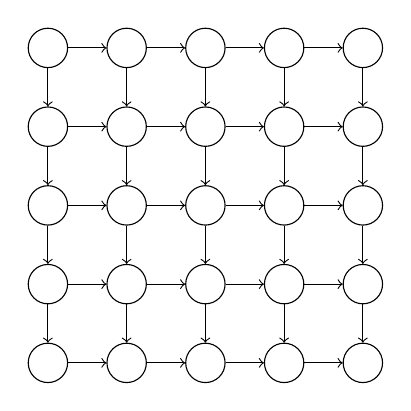
\begin{tikzpicture}[->, yscale = -1]
					\foreach \x in { 0, ..., 4 } {
						\foreach \y in { 0, ..., 4 } {
							\node [draw, circle, minimum width = 0.5cm, minimum height = 0.5cm, inner sep = 0] (n\x\y) at (\x, \y) {};
						}
					}

					\draw (n00) to (n10);
					\draw (n10) to (n20);
					\draw (n20) to (n30);
					\draw (n30) to (n40);
					\draw (n01) to (n11);
					\draw (n11) to (n21);
					\draw (n21) to (n31);
					\draw (n31) to (n41);
					\draw (n02) to (n12);
					\draw (n12) to (n22);
					\draw (n22) to (n32);
					\draw (n32) to (n42);
					\draw (n03) to (n13);
					\draw (n13) to (n23);
					\draw (n23) to (n33);
					\draw (n33) to (n43);
					\draw (n04) to (n14);
					\draw (n14) to (n24);
					\draw (n24) to (n34);
					\draw (n34) to (n44);

					\draw (n00) to (n01);
					\draw (n01) to (n02);
					\draw (n02) to (n03);
					\draw (n03) to (n04);
					\draw (n10) to (n11);
					\draw (n11) to (n12);
					\draw (n12) to (n13);
					\draw (n13) to (n14);
					\draw (n20) to (n21);
					\draw (n21) to (n22);
					\draw (n22) to (n23);
					\draw (n23) to (n24);
					\draw (n30) to (n31);
					\draw (n31) to (n32);
					\draw (n32) to (n33);
					\draw (n33) to (n34);
					\draw (n40) to (n41);
					\draw (n41) to (n42);
					\draw (n42) to (n43);
					\draw (n43) to (n44);
				\end{tikzpicture}
				\caption{Dependencies of pixels as assumed by a PixelRNN. Generation starts from the top left and propagates through the whole image.}
				\label{fig:pixelrnn}
			\end{figure}
		% end

		\subsection{Change of Variables}
			Instead of sampling from the actual distribution \( p(\vec{x}) \), it is possible to learn a mapping \( \vec{y} = \vec{g}(\vec{x}) \) such that
			\begin{equation}
				p_{\vec{x}}(\vec{x}) = p_{\vec{y}}\big( \vec{g}(\vec{x}) \big) \Biggl\lvert \det\biggl( \pdv{g(\vec{x})}{\vec{x}} \biggr) \Biggr\rvert.
			\end{equation}
			Then sampling can be done from the distribution \( p_{\vec{y}}(\vec{y}) \) instead and the results can be mapped back to the visible space.

			Disadvantages are that the transformation \(\vec{g}(\cdot)\) must be invertible and that the latent dimension must match the real dimension.
		% end

		\subsection{Boltzmann Machine}
			A \emph{Boltzmann machine} defines the likelihood as
			\begin{align}
				p(\vec{x}) &= \frac{1}{Z} \exp\bigl\{ -E(\vec{x}, \vec{z}) \bigr\} &
				Z &= \sum_{\vec{x}} \sum_{\vec{z}} \exp\bigl\{ -E(\vec{x}, \vec{z}) \bigr\}
			\end{align}
			As this is intractable, sampling requires Markov chain Monte Carlo methods.
		% end
	% end

	\section{Variational Auto-Encoder (VAE)}
		\label{sec:vae}

		While fully visible belief networks define a tractable density function \( p_{\vec{\theta}}(\vec{x}) = p_{\vec{\theta}}(x_1) \prod_{i = 2}^{n} p_{\vec{\theta}}(x_i \given \dotsrange{x_1}{x_{i - 1}}) \) that can be used to optimize the likelihood of the data, \emph{variational auto-encoders} (VAEs) define an intractable density function
		\begin{equation}
			p_{\vec{\theta}}(\vec{x}) = \int\! p_{\vec{\theta}}(\vec{z}) \, p_{\vec{\theta}}(\vec{x} \given \vec{z}) \dd{\vec{z}}
		\end{equation}
		using a latent representation \(\vec{z}\). This can not be used to directly optimize the likelihood. Instead, a lower bound is derived and optimized instead.

		This section will first introduce non-variational (classical) auto-encoders and subsequently lay down the definition of the VAE model, the derivation of the lower bound, and how to train and sample from the model

		\subsection{Auto-Encoder}
			An \emph{auto-encoder} is composed of two parts (usually neural networks): the \emph{encoder} and the \emph{decoder}. The encoder is used to compute a low-dimensional\footnote{Usually at least lower-dimensional than the original data.} feature representation \(\vec{z}\) from the original data. This feature representation is then passed to the decoder which reconstructs the original data. The latent dimension can then be used in various different ways: either to pass it to another model and exploit that the latent dimension is low-dimensional and has to contain meaningful information about the original data or to actually compress and transmit data. To achieve this, the encoder and decoder are trained jointly using an L2 loss between the input data and the reconstructed data. The boundary between the encoder and decoder is usually called the \emph{bottleneck} of the auto-encoder as it forces all data to be compressed into this dimensionality. \autoref{fig:autoEncoder} is an illustration of this concept.

			To generate new data from a classical auto-encoder, it is possible to sample latent vectors---but this does not work well. This is due to the vectors in the latent dimension being unrestricted at how the scatter across the whole space. Also it is unclear on how to actually sample the vectors because no distribution is defined within the latent space.

			\begin{figure}
				\centering
				\begin{tikzpicture}[yscale = -1]
					\coordinate (ea) at (-2, -1.4);
					\coordinate (eb) at (-1, -0.4);
					\coordinate (ec) at (-1, +0.4);
					\coordinate (ed) at (-2, +1.4);
					\path (eb) to coordinate(ebc) (ec);
					\path (ea) to coordinate(ead) (ed);
					\coordinate [left = 1 of ead, label = left:{\( \vec{x} \)}] (eadM);
					\path let \p1 = (eb), \p2 = (ea) in coordinate (eA) at (\x1, \y2);

					\coordinate (da) at (+2, -1.4);
					\coordinate (db) at (+1, -0.4);
					\coordinate (dc) at (+1, +0.4);
					\coordinate (dd) at (+2, +1.4);
					\path (db) to coordinate(dbc) (dc);
					\path (da) to coordinate(dad) (dd);
					\coordinate [right = 1 of dad, label = right:{\( \hat{\vec{x}} \)}] (dadM);
					\path let \p1 = (db), \p2 = (da) in coordinate (dA) at (\x1, \y2);

					\draw (ea) to (ed);
					\draw (eb) to (ec);
					\draw (da) to (dd);
					\draw (db) to (dc);

					\path (ea) to node[above]{Encoder} (eA);
					\path (da) to node[above]{Decoder} (dA);

					\path (ebc) to node(z){\(\vec{z}\)} (dbc);

					\draw [->] (ebc) to (z) to (dbc);
					\draw [->] (eadM) to (ead);
					\draw [->] (dad) to (dadM);

					\foreach \a in { -1.4, -1.0, ..., 1.4 } {
						\foreach \b in { -0.4, -0.0, ..., 0.4 } {
							\draw (-2, \a) to (-1, \b);
							\draw (+2, \a) to (+1, \b);
						}
					}
				\end{tikzpicture}
				\caption{Illustration of a classical auto-encoder.}
				\label{fig:autoEncoder}
			\end{figure}
		% end

		\subsection{Model and Evidence Lower Bound}
			As already seen in the previous section, auto-encoders work well in finding a low-dimensional embedding that explains the data and provides nonlinear mappings into and out of this embedding. A variational autoencoder is now an extension of classical auto-encoders that have a probabilistic interpretation and place a distribution on the latent space such that it can be sampled. Let \( p_{\vec{\theta}^\ast}(\vec{z}) \) be the true prior of the latent dimension and let \( p_{\vec{\theta}^\ast}(\vec{x} \given \vec{z}) \) be the true conditional. Usually the prior is chosen to be simple, e.g. a Gaussian, and the conditional distribution is represented by a neural network. This is called the decoder network and serves a similar purpose as in classical auto-encoders. To train the model, the data likelihood
			\begin{equation}
				p_{\vec{\theta}}(\vec{x}) = \int\! p_{\vec{\theta}}(\vec{z}) \, p_{\vec{\theta}}(\vec{x} \given \vec{z}) \dd{\vec{z}}  \label{eq:vaeLikelihood}
			\end{equation}
			is maximized. But this integral is intractable! And thus the posterior density
			\begin{equation}
				p_{\vec{\theta}}(\vec{z} \given \vec{x}) = \frac{p_{\vec{\theta}}(\vec{x} \given \vec{z}) \, p_{\vec{\theta}}(\vec{z})}{p_{\vec{\theta}}(\vec{x})}
			\end{equation}
			is also intractable because the normalization factor is intractable. The core idea of VAEs is to define an additional encoder network \( q_{\vec{\phi}}(\vec{z} \given \vec{x}) \) that approximates the true posterior \( p_{\vec{\theta}}(\vec{z} \given \vec{x}) \). This allows to derive a lower bound on the data likelihood that can be optimized end-to-end. When choosing a Gaussian distributions for the latents, the encoder and decoder networks are now two-headed: they both produce the mean and covariance\footnote{When implementing, it is often helpful to not let the network directly produce the covariance matrix or standard deviation, but rather the logarithm. This does not make a difference mathematically, but taking the logarithm afterwards (which will in the ELBO) would result in numerical instability as the network might produce negative numbers. Taking the logarithm implicitly circumvents this problem.} of the Gaussian, explicitly modeling the distributions.

			\subsubsection{Deriving the Lower Bound}
				To derive the ELBO, there are two approaches: one uses Jensen's inequality and the other does not. This section contains both of the derivations.

				\paragraph{With Jensen's Inequality}
					To derive the ELBO using Jensen's inequality, the data likelihood is first written according to \eqref{eq:vaeLikelihood}, and then massaged using statistical properties:
					\begin{align}
						\log p_{\vec{\theta}}(\vec{x})
							&= \log \int\! p_{\vec{\theta}}(\vec{z}) \, p_{\vec{\theta}}(\vec{x} \given \vec{z}) \dd{\vec{z}} \\
							&= \log \int\! q_{\vec{\phi}}(\vec{z} \given \vec{x}) \, \frac{p_{\vec{\theta}}(\vec{x} \given \vec{z}) \, p_{\vec{\theta}}(\vec{z})}{q_{\vec{\phi}}(\vec{z} \given \vec{x})} \dd{\vec{z}} \\
							&\geq \int\! q_{\vec{\phi}}(\vec{z} \given \vec{x}) \, \log \frac{p_{\vec{\theta}}(\vec{x} \given \vec{z}) \, p_{\vec{\theta}}(\vec{z})}{q_{\vec{\phi}}(\vec{z} \given \vec{x})} \dd{\vec{z}} \\
							&= \int\! q_{\vec{\phi}}(\vec{z} \given \vec{x}) \, \log p_{\vec{\theta}}(\vec{x} \given \vec{z}) \dd{\vec{z}} - \int\! q_{\vec{\phi}}(\vec{z} \given \vec{x}) \, \log \frac{q_{\vec{\phi}}(\vec{z} \given \vec{x})}{p_{\vec{\theta}}(\vec{z})} \dd{\vec{z}} \\
							&= \E_{\vec{z} \sim q_{\vec{\phi}}(\cdot \subgiven \vec{x})}\!\big[\! \log p_{\vec{\theta}}(\vec{x} \given \vec{z}) \big] - D_\mathrm{KL}\big( q_{\vec{\phi}}(\vec{z} \given \vec{x}) \,\Vert\, p_{\vec{\theta}}(\vec{z}) \big) \\
							&\eqqcolon \mathcal{L}_\mathrm{ELBO}(\vec{x}; \vec{\theta}, \vec{\phi})
					\end{align}
					In the second step the integrand was multiplied by one, the third step uses Jensen's inequality, and the rest is just moving around and exploiting of properties of the logarithm.
				% end

				\paragraph{Without Jensen's Inequality}
					To derive the ELBO without Jensen's inequality, the data likelihood is surrounded by a noop integral which can then be transformed into the ELBO:
					\begin{align}
						\log p_{\vec{\theta}}(\vec{x})
							&= \int\! q_{\vec{\phi}}(\vec{z} \given \vec{x}) \, \log p_{\vec{\theta}}(\vec{x}) \dd{\vec{z}} \\
							&= \int\! q_{\vec{\phi}}(\vec{z} \given \vec{x}) \, \log \frac{p_{\vec{\theta}}(\vec{x} \given \vec{z}) \, p_{\vec{\theta}}(\vec{z})}{p_{\vec{\theta}}(\vec{z} \given \vec{x})} \dd{\vec{z}} \\
							&= \int\! q_{\vec{\phi}}(\vec{z} \given \vec{x}) \, \log \frac{p_{\vec{\theta}}(\vec{x} \given \vec{z}) \, p_{\vec{\theta}}(\vec{z})}{p_{\vec{\theta}}(\vec{z} \given \vec{x})} \frac{q_{\vec{\phi}}(\vec{z} \given \vec{x})}{q_{\vec{\phi}}(\vec{z} \given \vec{x})} \dd{\vec{z}} \\
							&= \int\! q_{\vec{\phi}}(\vec{z} \given \vec{x}) \, \log p_{\vec{\theta}}(\vec{x} \given \vec{z}) \dd{\vec{z}} - \int\! q_{\vec{\phi}}(\vec{z} \given \vec{x}) \, \log \frac{q_{\vec{\phi}}(\vec{z} \given \vec{x})}{p_{\vec{\theta}}(\vec{z})} \dd{\vec{z}} + \int\! q_{\vec{\phi}}(\vec{z} \given \vec{x}) \, \log \frac{q_{\vec{\phi}}(\vec{z} \given \vec{x})}{p_{\vec{\theta}}(\vec{z} \given \vec{x})} \dd{\vec{z}} \\
							&= \E_{\vec{z} \sim q_{\vec{\phi}}(\cdot \subgiven \vec{x})}\!\big[\! \log p_{\vec{\theta}}(\vec{x} \given \vec{z}) \big] - D_\mathrm{KL}\big( q_{\vec{\phi}}(\vec{z} \given \vec{x}) \,\Vert\, p_{\vec{\theta}}(\vec{z}) \big) + \underbrace{D_\mathrm{KL}\big( q_{\vec{\phi}}(\vec{z} \given \vec{x}) \,\Vert\, p_{\vec{\theta}}(\vec{z} \given \vec{x}) \big)}_{\geq\, 0} \\
							&\geq \E_{\vec{z} \sim q_{\vec{\phi}}(\cdot \subgiven \vec{x})}\!\big[\! \log p_{\vec{\theta}}(\vec{x} \given \vec{z}) \big] - D_\mathrm{KL}\big( q_{\vec{\phi}}(\vec{z} \given \vec{x}) \,\Vert\, p_{\vec{\theta}}(\vec{z}) \big) \\
							&\eqqcolon \mathcal{L}_\mathrm{ELBO}(\vec{x}; \vec{\theta}, \vec{\phi})
					\end{align}
					The first step adds an integral over \(\vec{z}\) which is valid because \( p_{\vec{\theta}}(\vec{x}) \) does not depend on \(\vec{z}\) and is thus just a multiplicative constant w.r.t. the integral. In the second step the data likelihood is written out using Bayes' rule. The third step multiplies the argument of the logarithm with a one, not changing the overall value. Then, in the fourth step, the integral can be split into three parts by exploiting properties of the logarithm. This yields, in the fifth step, three components: a tractable expectation, a tractable KL-divergence and an intractable KL-divergence. As the latter it always non-negative it can be discarded in the sixth step, yielding the ELBO (seventh step).

					While this derivation is a tad longer than the derivation using Jensen's inequality, it fives some more insights on what the ELBO is actually neglects: the KL-divergence, or distance, between the approximate posterior and the actual posterior. Thus it is possible that optimizing the ELBO does not even closely approximate the true posterior as it is not enforced. But as the first and second part of the ELBO ensure reconstruction and staying close to the prior, respectively, optimizing it usually yields good embeddings.
				% end
			% end
		% end

		\subsection{Training Procedure and Generating Data}
			To optimize a VAE, the ELBO has to be maximized. This is done by computing a forward pass through the network and both sampling layers and backpropagating through it. As it is not possible to differentiate a sampling procedure per se, a trick called the \emph{reparametrization trick} is used: instead of directly sampling from the encoder distribution, samples are taken from a fixed distribution and are transformed via the sufficient statistics produced by the encoder network. For a Gaussian \( q_{\vec{\phi}}(\vec{z} \given \vec{x}) = \mathcal{N}(\vec{z} \given \vec{\mu}_{\vec{x}}, \mat{\Sigma}_{\vec{x}}) \), where the mean and covariance are produced by the encoder network, the latent variables are not sampled directly from \( q_{\vec{\phi}} \), but an auxiliary variable \( \vec{\epsilon} \) is sampled from a unit Gaussian. This sample is then transformed using the mean and covariance like it has been sampled from the posterior directly:
			\begin{equation}
				\vec{z} \sim \mathcal{N}(\vec{z} \given \vec{\mu}_{\vec{x}}, \mat{\Sigma}_{\vec{x}})
				\qquad\implies\qquad
				\vec{z} = \vec{\mu}_{\vec{x}} + \mat{\Sigma}_{\vec{x}}^{1/2} \vec{\epsilon},\quad \vec{\epsilon} \sim \mathcal{N}(\vec{0}, \mat{I})
			\end{equation}
			Here \( \mat{\Sigma}_{\vec{x}}^{1/2} \) is the Cholesky decomposition of the covariance matrix.

			To generate samples from the VAE, it is now possible to just sample from the prior and push the result through the decoder network. When a diagonal prior was used (like it is usually done), the latent variables are independent and different dimensions of \(\vec{z}\) might encode interpretable information about the data. This is also a good feature representation that can be used in subsequent models.
		% end

		\subsection{Pros and Cons}
			The advantages of VAEs are that they are a principled approach to generative models and allow inference of \( q_{\vec{\phi}}(\vec{z} \given \vec{x}) \) which exhibits useful feature representations for other tasks. Disadvantages are that the maximization of the ELBO work reasonable well, but is not an evaluation metric as good as the density in PixelRNN/PixelCNN. Also the samples are blurrier and of lower quality compared to state-of-the-art generative models (Generative Adversarial Models, GANs).

			But they are extremely flexibly and allow rich approximations of the posterior, also more than Gaussian distributions. They also incorporate structure in the latent variables that allow for interpretability.
		% end
	% end

	\section{Generative Adversarial Networks}
		\emph{Generative adversarial networks} (GANs) take a step back and give up explicitly modeling the density \( p(\vec{x}) \) in the favor of specializing on generating data. This is done by training two networks jointly: the generator network \( G_{\vec{\theta}_g(\vec{z})} \) which has the only requirement of being differentiable---especially not necessarily invertible---and the discriminator network \( D_{\vec{\theta}_d}(\vec{x}) \) which must also be differentiable. The generator network is used for transforming the \emph{noise vector} \(\vec{z}\), which is usually sampled from a simple distribution, into output data \(\vec{x}\) (often these are images). Hence, it "generates" images. For some theoretical guarantees the noise vector must be of higher dimension than the image dimensionality, but this is not a necessity. The discriminator network then tries to distinguish real and fake images by assigning each input data a probability of it being real.

		The next sections will cover the training process and the model in more detail and glimpse at some related network architectures.

		\subsection{Training Procedure}
			Training a GAN is done using a gradient descent variant like Adam on two batches of data simultaneously: the first batch are real images, the training examples, and the second batch are fake images generated by the generator network. Both networks are then trained simultaneously in a minimax game
			\begin{equation}
				\min_{\vec{\theta}_g} \max_{\vec{\theta}_d} \; \E_{\vec{x} \sim p_\mathrm{data}(\cdot)}\big[\! \log D_{\vec{\theta}_d}(\vec{x}) \big] + \E_{\vec{z} \sim p(\vec{z})}\Big[\! \log\!\Big(\! 1 - D_{\vec{\theta}_d}\big( G_{\vec{\theta}_g}(\vec{z}) \big) \!\Big) \Big]
			\end{equation}
			where the two expectations are (as usual) approximated using minibatches of data. The first expectation describes the log-likelihood that the discriminator classifies the real images correctly and the second expectation described the log-likelihood that the discriminator classifies the fake images correctly. As the discriminator maximizes and the generator minimizes the objective, the goal of the former is to correctly classify all data while the goal of the latter is to fool the discriminator. To optimize this objective, the training process alternates between gradient ascent on the discriminator and gradient descent on the generator parameters.

			The problem of this approach is that training the generator does not work well. This is because the loss in the regions where a sample is likely fake, i.e., not good enough, is relatively flat compared to regions where samples are already good. Hence, the gradient vanishes and no learning happens. This is due to the minimax game having an equilibrium at the saddle point of the loss. Do circumvent this, the training process must not alternate between minimizing and maximizing the same loss w.r.t. different parameters, but instead perform alternating gradient ascent on two different objectives:
			\begin{align}
				\max_{\vec{\theta}_d} \;& \E_{\vec{x} \sim p_\mathrm{data}(\cdot)}\big[\! \log D_{\vec{\theta}_d}(\vec{x}) \big] + \E_{\vec{z} \sim p(\vec{z})}\Big[\! \log\!\Big(\! 1 - D_{\vec{\theta}_d}\big( G_{\vec{\theta}_g}(\vec{z}) \big) \!\Big) \Big] \\
				\max_{\vec{\theta}_g} &\; \E_{\vec{z} \sim p(\vec{z})}\big[\! \log D_{\vec{\theta}_d}\big( G_{\vec{\theta}_g}(\vec{z}) \big) \big]
			\end{align}
			This is essentially the same, but now the equilibrium is no longer describable with a single loss and the minimax game is non-saturating. But this is also heuristically motivated! But it has the advantage that the generator can also learn when the discriminator successfully rejects all generator samples, making it kind of robust towards a too good discriminator.

			% TODO: GAN: Maximum Likelihood Objective; 9a.20

			It is also possible to view GANs as cooperative rather than adversarial games by interpreting the output of the discriminator as an estimate of the data and model distributions. The discriminator then "informs" the generator over its estimate such that the generate can improve itself. This is based on the fact the optimal discriminator distributions is
			\begin{equation}
				D(\vec{x}) = \frac{p_\mathrm{data}(\vec{x})}{p_\mathrm{data}(\vec{x}) + p_\mathrm{model}(\vec{x})}
			\end{equation}
			and the generator tries to estimate the real distribution: \( p_\mathrm{model}(\vec{x}) \approx p_\mathrm{data}(\vec{x}) \). If the generator would be optimal, \( p_\mathrm{model}(\vec{x}) = p_\mathrm{data}(\vec{x}) \), even the optimal discriminator would output \( D(\vec{x}) = 1/2 \), which is equivalent to random guess.

			Two remaining problems of GANs are that optimizing the objective is still unstable which lies in the nature oj jointly training two networks. This is an open area of research! Another problem is the \emph{mode collapse}: fully training the discriminator while the generator is held constant is safe and probably yields a good discriminator. But fully training the generator while the discriminator is fixed results in a generator that maps all inputs to the argmax of the discriminator, overfitting on the current discriminator and exploiting its weaknesses rather than learning to generate good samples. This can partially be fixed by adding nearest-neighbor features to the discriminator that are constructed from the current minibatch (\emph{minibatch GAN}).
		% end

		\subsection{Convolutional Architectures}
			Convolutional GANs use super-sampling in the generator with convolutions using a fractional stride, i.e., the stride is a fraction and thus pixels are used multiple times, resulting in a activation output volume, and a vanilla CNN architecture for the discriminator. Some more tips for designing CNN GANs are:
			\begin{itemize}
				\item Replace pooling layers with convolutions with stride in the discriminator and with convolutions with fractional stride in the generator.
				\item Use batch normalization in both networks.
				\item Remove fully connected layers for deeper architectures.
				\item Use ReLU activations for every layer in the generator except for the output which uses tanh.
				\item Use leaky ReLU activations for every layer in the discriminator.
			\end{itemize}
			Using CNN architectures as GANs results in high-definition images that look extremely realistic.
		% end

		\subsection{Vector Space Arithmetic}
			Basic arithmetic on the noise vectors \(\vec{z}\) can yield interesting interpretable results. If, for instance, a noise vector \( \vec{z}_\text{woman} \) generates a woman, \( \vec{z}_\text{man} \) generates a man without glasses, and \( \vec{z}_\text{glasses} \) generates a man with glasses, then \( \vec{z}_\text{glasses} - \vec{z}_\text{man} + \vec{z}_\text{woman} \) results in a woman with glasses. To use these properties it is of course necessary to get the corresponding noise vectors at first. But when using sufficiently low-dimensional noise vectors, finding the correct ones should not be too hard.
		% end

		\subsection{Pros and Cons}
			A big advantage of GANs is that they generate beautiful, state-of-the-art samples and images. The downsides on the other hand are that they are a lot trickier to train compared to, for example, VAEs and that they can not solve inference queries such as \( p(\vec{x}) \) and \( p(\vec{z} \given \vec{x}) \) as GANs do not model the distributions explicitly.

			Active areas of research regarding GANs are better loss functions that induce a more stable training (Wasserstein GAN, LSGAN, etc.), Conditional GANs for training multi-purpose GANs, and many more.
		% end
	% end

	\section{Optimization and Game Theory}
		Optimization and game theory are two topics that should not be viewed independently and have lots of links between them. In optimization, the goal is to find a set of parameters \( \vec{\theta}^\ast \) that are optimal w.r.t. some loss \( J(\vec{\theta}) \):
		\begin{equation}
			\vec{\theta}^\ast = \arg\min_{\vec{\theta}} \; J(\vec{\theta})
		\end{equation}
		In game theory (or, more specifically, a two-player game), there ate two sets of parameters: \( \vec{\theta}_1 \) and \( \vec{\theta}_2 \). The first player controls \(\vec{\theta}_1\) and tries to minimize its objective \( J_1(\vec{\theta}_1, \vec{\theta}_2) \) and the second players controls \(\vec{\theta}_2\) and tries to minimize its objective \( J_2(\vec{\theta}_1, \vec{\theta}_2) \). Depending on these losses, the game is either cooperative or non-cooperative. Optimization can therefore be viewed as a subset of the more general two-players games by setting \( \vec{\theta}_1 = \vec{\theta} \), \( \vec{\theta}_2 = \emptyset \), \( J_1(\vec{\theta}_1, \vec{\theta}_2) = J(\vec{\theta}_1) \), and \( J_2(\vec{\theta}_1, \vec{\theta}_2) = 0 \).

		A solution of a non-cooperative is characterized by its \emph{Nash equilibrium}. In a Nash equilibrium \( \vec{\theta}_1^\ast \), \( \vec{\theta}_2^\ast \), neither player can reduce its loss by changing their own strategy/parameters:
		\begin{align}
			\forall \vec{\theta}_1 : \eqmakebox[gtJBox][r]{\( \displaystyle  J_1 \)}(\vec{\theta}_1, \vec{\theta}_2^\ast) \geq \eqmakebox[gtJBox][r]{\( \displaystyle  J_1 \)}(\vec{\theta}_1^\ast, \vec{\theta}_2^\ast) \\
			\forall \vec{\theta}_2 : \eqmakebox[gtJBox][r]{\( \displaystyle  J_2 \)}(\vec{\theta}_1^\ast, \vec{\theta}_2) \geq \eqmakebox[gtJBox][r]{\( \displaystyle  J_2 \)}(\vec{\theta}_1^\ast, \vec{\theta}_2^\ast)
		\end{align}
		In other words: each player's loss is minimal with respect to the other player's strategy. Finding Nash equilibria can thus be seen again as a subset of optimization as a Nash equilibrium always characterized the global optimum.

		Some well-studies cases for games are finite minimax games (zero-sum games), finite mixed-strategy games, continuous and convex games, and differential games. In continuous games, the Nash equilibrium is a saddle point of the losses. More specifically, it has to be a maximum for one and a minimum for the other player. A necessary condition for an optima are---as usual---that the gradient of the loss vanishes and that the Hessian is positive semi-definite. A sufficient condition is that the Hessian is positive definite.

		This yields sufficient conditions for gradient descent to converge for both players. Given the joint gradient
		\begin{equation}
			\vec{\omega} =
				\begin{bmatrix}
					\grad_{\vec{\theta}_1} J_1(\vec{\theta}_1, \vec{\theta}_2) \\
					\grad_{\vec{\theta}_2} J_2(\vec{\theta}_1, \vec{\theta}_2)
				\end{bmatrix}
		\end{equation}
		the Eigenvalues of the \emph{generalized Hessian}
		\begin{equation}
			\grad_{\vec{\theta}_1, \vec{\theta}_2} \vec{\omega} =
				\begin{bmatrix}
					\grad_{\vec{\theta}_1} \grad_{\vec{\theta}_1} J_1(\vec{\theta}_1, \vec{\theta}_2) & \grad_{\vec{\theta}_1} \grad_{\vec{\theta}_2} J_2(\vec{\theta}_1, \vec{\theta}_2) \\
					\grad_{\vec{\theta}_2} \grad_{\vec{\theta}_1} J_1(\vec{\theta}_1, \vec{\theta}_2) & \grad_{\vec{\theta}_2} \grad_{\vec{\theta}_2} J_2(\vec{\theta}_1, \vec{\theta}_2)
				\end{bmatrix}
		\end{equation}
		must have a positive real part. This condition can be interpreted as each player's Hessian should have large, positive, Eigenvalues, expressing a strong urge to keep their strategy. The Jacobian of the gradient of one player w.r.t. the other player's strategy should have a small effect on the Eigenvalues, meaning that the change of strategy of the player has only a limited ability to change the other player's behavior. But sadly this does not apply to GANs, so their convergence still is an open question.

		Some heuristics for finding equilibria are to keep the parameter values close to their running average and periodically assign the running average to the parameters. Also add a loss for deviation from the running average.

		Other games in artificial intelligence are for example robust optimization and robust control, domain-adversarial learning for domain adaption, adversarial privacy, guided cost learning, and predictability minimization.
	% end
% end

\chapter{Probabilistic Graphical Models}
	This chapter introduces \emph{probabilistic graphical models} and \emph{tractable inference}. The core if inference is to answer given queries \(q\), for example "What is the probability that today is a Monday and there is a traffic jam on Herzl Str.?" Instead of fitting a predictive model, inference takes the step of formulating these kinds of queries statistically over a given model \(m\) of the world. The said query could be expressed as the probability \( q(m) = p_{m}(\text{Day} = \text{Monday},\, \text{Jam}_\text{Herzl} = 1) \). Other types of queries are also possible and different types of these will be discussed in \autoref{subsec:queries}.

	For a given family \(\mathcal{M}\) of models, a class of queries \(\mathcal{Q}\) is called \emph{tractable on \(\mathcal{M}\)} iff for any query \( q \in \mathcal{Q} \) and model \( m \in \mathcal{M} \), computing \( q(m) \) has time complexity \( \mathcal{O}\big( \mathrm{poly}(\lvert m \rvert \, \lvert q \rvert) \big) \) where \( \mathrm{poly}(\cdot) \) is any polynomial but is in practice often linear. Also, if \(\mathcal{M}\) and \(\mathcal{Q}\) are compact in the number of random variables \(\vec{X}\), i.e. \( \lvert m \rvert, \lvert q \rvert \in \mathcal{O}\big( \mathrm{poly}(\lvert \vec{X} \rvert) \big) \), then the query time is in \( \mathcal{O}\big( \mathrm{poly}(\lvert \vec{X} \rvert) \big) \).

	It is also possible to do \emph{approximate} inference instead of exact inference, but this brings some caveats: firstly, if it is possible to to exact inference, why do approximate inference? This can be answered in the context of tractability vs. expressiveness which is discussed in \autoref{sec:tractability}. Also, approximate inference can be intractable as well---but sometimes it comes with certain guarantees. But even those guarantees might not be enough and can mislead learners when the approximation is incorrect. It is also possible to do approximate inference by using exact inference in an approximate model. This is something one often has to resort to as the model is usually not exact.

	The next content of this chapter will be the different query types that are possible as well as certain concrete models and their pros and cons in terms of tractability and expressiveness. Afterwards probabilistic circuits and how to build them is covered and some applications are presented.

	\section{Tractability vs. Expressiveness}
		The core problem in inference is that more tractable queries and models are not very expressive whereas expressive models are usually not very tractable. This is known as the tractability vs. expressiveness tradeoff. To understand more what this means, the next section introduces the different variants of queries that can occur and the section after that highlights some models and their respective complexity on the queries.

		\subsection{Inference and Queries}
			\label{subsec:queries}

			As already said, this section will cover different query types and some examples of what such a query might encode.

			\subsubsection{Complete Evidence Queries (EVI)}
				\emph{Complete evidence} (EVI) queries ask for the probability of all random variables having specific values. This comes down to evaluating the complete joint probability. An example natural language query is
				\begin{center}
					"What is the probability that today is a Monday at 12pm and there is a traffic jam only on Herzl Str.?"
				\end{center}
				where all random variables are the day, the time, and whether there is a traffic jam for every street. The formalized version is
				\begin{equation}
					q(m) = p_m(\text{Day} = \text{Monday},\, \text{Time} = \text{12pm},\, \text{Jam}_\text{Herzl} = 1,\, \dotsrange{\text{Jam}_{\text{Str}2} = 0}{\text{Jam}_{\text{Str}N} = 0})
				\end{equation}
				and the general version is
				\begin{equation}
					p_m(\vec{Q} = \vec{q}).
				\end{equation}
				This kind of query is essential in maximum likelihood learning where the joint distribution is computed for every data point.
			% end

			\subsubsection{Marginal Queries (MAR)}
				\emph{Marginal} (MAR) queries ask for the probability of some random variables having specific values. This comes down to evaluating the marginal probability of the said random variables. An example natural language query is
				\begin{center}
					"What is the probability that today is a Monday \sout{at 12pm} and there is a traffic jam \sout{only} on Herzl Str.?"
				\end{center}
				where the time and other streets are marginalized out. The formalized version is
				\begin{equation}
					q(m) = p_m(\text{Day} = \text{Monday},\, \text{Jam}_\text{Herzl} = 1)
				\end{equation}
				and the general version is
				\begin{equation}
					p_m(\vec{Q} = \vec{q}) = \int\! p_m(\vec{Q} = \vec{q}, \vec{H} = \vec{h}) \dd{\vec{h}}
				\end{equation}
				with \( \vec{Q} \subseteq \vec{X} \) and \( \vec{H} = \vec{X} \setminus \vec{Q} \).
			% end

			\subsubsection{Conditional Queries (CON)}
				\emph{Conditional} (CON) queries ask for the probability of some random variables having specific values given that other random variables are known to have specific values. This comes down to evaluating the conditional probability of the said setting. An example natural language query is
				\begin{center}
					"What is the probability that these is a traffic jam on Herzl Str. \emph{given that} today is a Monday?"
				\end{center}
				where the day is the given random variable. The formalized version is
				\begin{equation}
					q(m) = p_m(\text{Jam}_\text{Herzl} = 1 \given \text{Day} = \text{Monday})
				\end{equation}
				and the general version is
				\begin{equation}
					p_m(\vec{Q} = \vec{q} \given \vec{E} = \vec{e}) = \frac{p_m(\vec{Q} = \vec{q}, \vec{E} = \vec{e})}{p_m(\vec{E} = \vec{e})}
				\end{equation}
				with \( \vec{Q} \subseteq \vec{X} \), \( \vec{E} \subseteq \vec{X} \), and \( \vec{Q} \cap \vec{E} = \emptyset \). As conditional probabilities can be purely expressed using marginals, the ability to answer CON queries follows from the ability of answering MAR queries.
			% end

			\subsubsection{Maximum A-Posteriori (MAP)}
				\emph{Maximum a-posteriori} (MAP) or \emph{most probable explanation} (MPE) queries ask for the values of some random variables that are most likely given other random variables are known to have specific values. The combination of variables in question and given variables has to be exhaustive. This comes down to evaluating the configuration of the random variables in question that maximizes the posterior probability. An example natural language query is
				\begin{center}
					"Which combination of streets is most likely to be jammed on Monday at 12pm?"
				\end{center}
				where the configuration of streets are the random variables that is asked for and day and time are the given random variables. The formalized version is
				\begin{equation}
					q(m) = \arg\max_{\subdotsrange{j_1}{j_N}} \; p_m(\dotsrange{\text{Jam}_{\text{Str}1} = j_1}{\text{Jam}_{\text{Str}N} = j_N} \given \text{Day} = \text{Monday},\, \text{Time} = \text{12pm})
				\end{equation}
				and the generalized version is
				\begin{equation}
					\arg\max_{\vec{q}} \; p_m(\vec{Q} = \vec{q} \given \vec{E} = \vec{e})
				\end{equation}
				with \( \vec{Q} \subseteq \vec{X} \), \( \vec{E} \subseteq \vec{e} \), \( \vec{Q} \cap \vec{E} = \emptyset \), and \( \vec{Q} \cup \vec{E} = \vec{X} \).

				These kinds of queries are intractable for latent variable models!
			% end

			\subsubsection{Marginal MAP (MMAP)}
				\emph{Marginal maximum a-posteriori} (MMAP) queries ask for the values of some random variables that are most likely given other random variables are known to have specific values. The combination of variables in question and given variables dows not have to be exhaustive. This comes down to evaluating the configuration of the random variables in question that maximizes the marginal posterior probability. An example natural language query is
				\begin{center}
					"Which combination of streets is most likely to be jammed \sout{on Monday} at 12pm?"
				\end{center}
				where the configuration of streets are the random variables that is asked for and the day is marginalized out. The formalized version is
				\begin{equation}
					q(m) = \arg\max_{\subdotsrange{j_1}{j_N}} \; p_m(\dotsrange{\text{Jam}_{\text{Str}1} = j_1}{\text{Jam}_{\text{Str}N} = j_N} \given \text{Time} = \text{12pm})
				\end{equation}
				and the generalized version is
				\begin{equation}
					\arg\max_{\vec{q}} \; p_m(\vec{Q} = \vec{q} \given \vec{E} = \vec{e})
						= \arg\max_{\vec{q}} \; \sum_{\vec{h}} p_m(\vec{Q} = \vec{q}, \vec{H} = \vec{h} \given \vec{E} = \vec{e})
				\end{equation}
				with \( \vec{Q} \cup \vec{H} \cup \vec{E} = \vec{X} \).

				These kinds of queries are \( \mathit{NP}^\mathit{PP} \)-complete, \( \mathit{NP} \)-hard for trees, and even \(\mathit{NP}\)-hard for naive Bayes!
			% end

			\subsubsection{Advanced Queries}
				More advanced queries might combine several of the ones introduced above, for example
				\begin{center}
					"Which day is most likely to have a traffic jam on my route to work?"
				\end{center}
				and
				\begin{center}
					"What is the probability of seeing more traffic jams in Jaffa than Marina?"
				\end{center}
				The former needs marginals and maximum a-posteriori and logical events and can be formalized as
				\begin{equation}
					q(m) = \arg\max_{\text{day}} \; p_m\Big(\text{Day} = \text{day},\, \textstyle\bigvee_{i \,\in\, \text{Route}}\displaystyle \text{Jam}_{\text{Str}i} = 1\Big)
				\end{equation}
				and the latter needs counts and group comparisons. These kinds of queries can get very complex very fast.
			% end
		% end

		\subsection{Models}
			This section will introduce some models in different levels of detail and relate them to the different query types introduces beforehand in terms of tractability and expressiveness.

			\subsubsection{GANs and VAEs}
				GANs are powerful generative models that can generate good-looking samples, but they do not serve well for inference. That is due to the lack of an explicit likelihood and hence EVI is not tractable. Also the training is unstable due to the mode collapse and lots of samples are needed for effective Monte Carlo inference.

				Similar goes for VAEs. They serve an explicit likelihood model, but computing \( \log p_{\vec{\theta}}(\vec{x}) \) is intractable as it is an infinite and uncountable mixture of distributions. Hence, EVI is not tractable. Also, the ELBO has to be optimized instead of the real data likelihood which is "broken"\footnote{Alexander Alemi, Ben Poole, Ian Fischer, Joshua Dillon, Rif A. Saurous, and Kevin Murphy (2018): "Fixing a Broken ELBO"}\footnote{Bin Dai and David Wipf (2019): "Diagnosing and Enhancing VAE Models"}.
			% end

			\subsubsection{Mixture Models}
				\emph{Mixture models} are built by combining multiple simpler models
				\begin{equation}
					p(\vec{X}) = w_1 p_1(\vec{X}) + w_2 p_2(\vec{X}),
				\end{equation}
				e.g. Gaussians. They can be seen as a marginalization over a categorical latent variable \(Z\) that describes the amount one of the distributions participates to the mixture model. This increases the expressiveness of the simpler distributions.

				In fact, a mixture of Gaussians can represent any distribution, but this would need lots of Gaussians. This is known as \emph{expressive efficiency}, settings the expressiveness of a model in relation to its complexity/size.
			% end

			\subsubsection{Probabilistic Graphical Models: Markov and Bayes Networks}
				Probabilistic graphical models are---in a nutshell---a graphical notation for conditional independence assumptions and a compact representation for probability distributions. They utilize graphs where the nodes represent random variables and the edges represent dependencies between them. They divide into three main types: \emph{Markov networks}, \emph{Bayesian networks}, and \emph{factor graphs}. Markov networks and Bayesian networks are closely related with the difference that the edges in Bayesian networks are directed while they are not in Markov networks. Factor graphs are a more general form of PGMs than can represent all kinds of relations, including everything that can be represented using a Markov or Bayesian network.

				In general, exact inference for MAR and CON queries in PGMs is \(\mathrm{\#P}\)-complete. Also approximate inference of MAR and CON queries with a relative error of \( 2^{n^{1 - \epsilon}} \) for any fixed \(\epsilon\) is \(\mathrm{NP}\)-hard. The complexity can be further refined using the \emph{treewidth} of a PGM. The treewidth \(w\) described how tree-like a graphical model \(m\) is. Formally, it is the minimum width of any tree-decomposition of \(m\). With that number, the time complexity of MAR and CON queries on a graphical model with treewidth \(w\) is \( \mathcal{O}(2^w \, \lvert \vec{X} \rvert) \), which is linear for a fixed \(w\). One idea is to bound the tree-width by design as inference is possible in practice for \( w \approx 20 \). The extreme form are trees which are covered after Bayesian networks as they are a special form of them.

				\paragraph{Fully Factorized Models}
					\emph{Fully factorized models} are PGMs with no connections between the random variables. That is, each random variable is independent from all others and EVI, MAR, MAP, and MMAP inference is linear in time. But these models are definitely not expressive.
				% end

				\paragraph{Bayesian Networks and Variable Elimination}
					Bayesian networks are digraphs in which every node is a random variable and all parents of that not are dependencies. \autoref{fig:bayesNetExample} shows an example of a Bayesian network that describes the joint distribution
					\begin{equation}
						P(A, B, C, D, E) = P(A) \, P(B) \, P(C \given A, B) \, P(D \given B) \, P(E \given C).
					\end{equation}
					In general, the joint distributions for a Bayesian network with the random variables \( \dotsrange{X_1}{X_N} \) is described by
					\begin{equation}
						P(\dotsrange{X_1}{X_N}) = \prod_{i = 1}^{N} P\big( X_i \biggiven \mathrm{Pa}(X_i) \big)
					\end{equation}
					where \( \mathrm{Pa}(X_i) \) is the set of parents of the random variable \( X_i \). In the example shown in \autoref{fig:bayesNetExample}, this would, for example, be \( \mathrm{Pa}(C) = \{ A, B \} \). The local Markov assumption in Bayesian networks is that each random variable is independent from its non-descendants given its parents. As the joint distribution can be computed efficiently, EVI queries are tractable!

					To evaluate MAR queries, an algorithm called \emph{variable elimination} can be used. It is based on the observation that in the general form of a marginalization,
					\begin{equation}
						P(\vec{Q}) = \sum_{X_j \,\not\in\, \vec{Q}}^{\text{marg}} \prod_{i = 1}^{N} P\big( X_i \biggiven \mathrm{Pa}(X_i) \big),
					\end{equation}
					where the first sum described a marginalization on its summation index, i.e., a summation of all possible realizations of \(X_j\), the product and the sum can be exchanged under certain circumstances. That is, if all of the factors are independent of a variable \(X_k\), these factors can be pulled before the sum:
					\begin{align}
						P(\vec{Q})
							&= \sum_{X_j \,\not\in\, \vec{Q}}^{\text{marg}} \prod_{i = 1}^{N} P\big( X_i \biggiven \mathrm{Pa}(X_i) \big) \\
							&= \prod_{\substack{i \,=\, 1 \\ X_k \,\not\in\, \{ X_i \} \,\cup\, \mathrm{Pa}(X_i)}}^{N} \hspace{-1.06cm} P\big( X_i \biggiven \mathrm{Pa}(X_i) \big) \sum_{X_j \,\not\in\, \vec{Q}}^{\text{marg}} \prod_{\substack{i \,=\, 1 \\ X_k \,\in\, \{ X_i \} \,\cup\, \mathrm{Pa}(X_i)}}^{N} \hspace{-1.06cm} P\big( X_i \biggiven \mathrm{Pa}(X_i) \big)
					\end{align}
					This way not the complete joint has to be computed for each combination of the random variables that are marginalized out. \autoref{alg:variableElimination} shows the pseudocode for this algorithm.

					But even with this rather efficient algorithm, inference in Bayesian networks is still NP-hard!

					\begin{figure}
						\centering
						\begin{tikzpicture}[->, every node/.style = { draw, circle, minimum width = 1cm, minimum height = 1cm }]
							\node (a) {\(A\)};
							\node [below = 1.5 of a] (b) {\(B\)};
							\node [right = 1.5 of a] (c) {\(C\)};
							\node [right = 1.5 of b] (d) {\(D\)};
							\node [right = 1.5 of c] (e) {\(E\)};

							\draw (a) -> (c);
							\draw (b) -> (c);
							\draw (b) -> (d);
							\draw (c) -> (e);
						\end{tikzpicture}
						\caption{Example of a Bayesian network with the random variables \(A\), \(B\), \(C\), \(D\), and \(E\).}
						\label{fig:bayesNetExample}
					\end{figure}

					\begin{algorithm}  \DontPrintSemicolon
						\KwIn{Query \( P(\vec{Q}) \).}
						\KwOut{Probability \( P(\vec{Q}) \).}
						Initialize factors \( \mathcal{F} = \{ \dotsrange{f_1}{f_N} \} \) with \( f_i = P\big( X_i \biggiven \mathrm{Pa}(X_i) \big) \) \;
						\For{\( i = \dotsrange{1}{N} \)}{
							\If{\( X_i \in \vec{Q} \)}{
								\textit{skip} \;
							}

							Collect factors \( \dotsrange{f_1}{f_k} \) that contain \(X_i\). \;
							\tcp{Generate a new factor by eliminating \(X_i\) from these factors:}
							\( \displaystyle  g = \sum_{X_i}^{\text{marg}} \prod_{j = 1}^{k} f_j \) \;
							\tcp{Add \(g\) to the set of factors:}
							\( \displaystyle  \mathcal{F} \gets \mathcal{F} \cup \{ g \} \) \;
						}
						Factors \(\mathcal{F}\) now include \( P(\vec{Q}) \). \;
						\caption{Variable Elimination}
						\label{alg:variableElimination}
					\end{algorithm}
				% end

				\paragraph{Low-Treewidth PGMs: Trees}
					If in a Bayesian network every random variable has at most one parent, the Bayesian network is a \emph{tree}. Then EVI, MAR, and CON queries can be answered exactly in linear time \( \mathcal{O}( \lvert \vec{X} \rvert ) \). Also, exact learning from \(d\) samples takes \( \mathcal{O}(d \, \lvert \vec{X} \rvert^2) \) with the Chow-Liu algorithm.

					This comes at the cost of not being able to represent rich and complex classes of distributions. In general, bounded-treewidth PGMs lose the ability to represent all possible distributions.
				% end
			% end
		% end
	% end

	\section{Probabilistic Circuits} % 10b.104, 10b.126
		\emph{Probabilistic circuits} are computational graphs for probabilistic models. They are built from simple distributions as building blocks and summation and multiplication between them.

		The starting point (base case) are univariate distributions, i.e. distributions over scalars. Generally they are tractable for EVI (by answering the value of the density/mass at the query point), MAR (bay answering \num{1} if normalized or \(Z\)), and MAP queries (by answering the location of the mode). The univariate building block is written as
		\begin{center}
			\begin{tikzpicture}[->, comp/.style = { draw, circle, minimum width = 0.75cm, minimum height = 0.75cm, inner sep = 0 }]
				\coordinate [label = left:{\(x\)}] (a);
				\node [comp, right = 1 of a] (b) {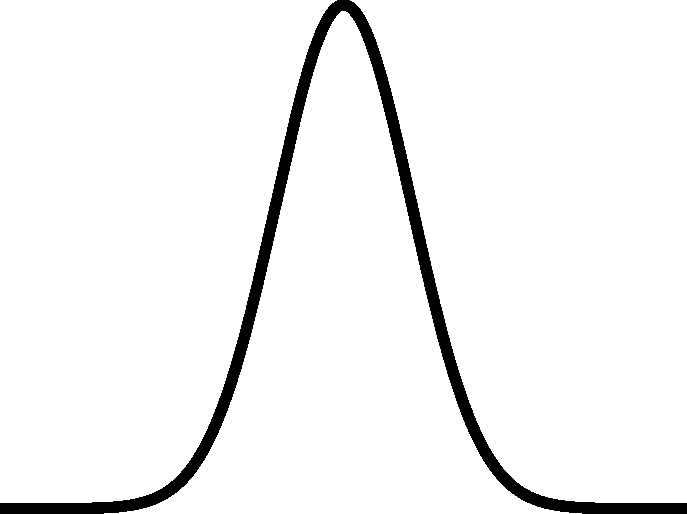
\includegraphics[width=0.5cm]{img/gaussian.pdf}};
				\coordinate [right = 1 of b, label = right:{\(p(x)\)}] (c);
				\draw (a) to (b);
				\draw (b) to (c);
			\end{tikzpicture}
		\end{center}
		as they are usually Gaussians. Multiple univariate probabilities can also be multiplied which is denoted as
		\begin{center}
			\begin{tikzpicture}[->, comp/.style = { draw, circle, minimum width = 0.75cm, minimum height = 0.75cm, inner sep = 0 }]
				\node [comp] (a) {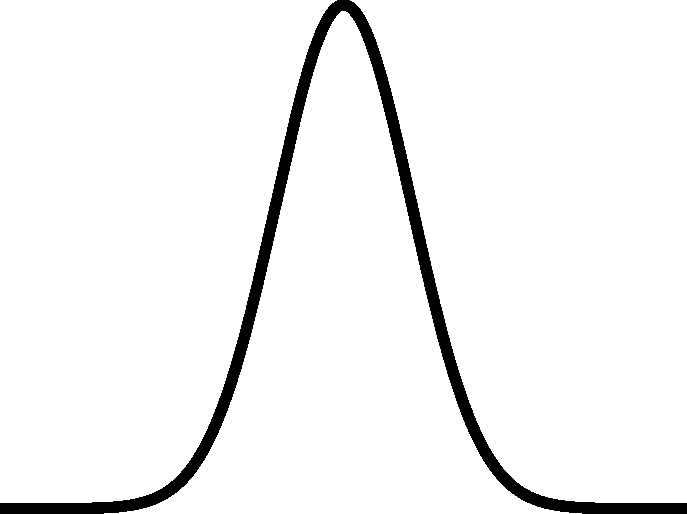
\includegraphics[width=0.5cm]{img/gaussian.pdf}};
				\node [comp, below = 0.5 of a] (b) {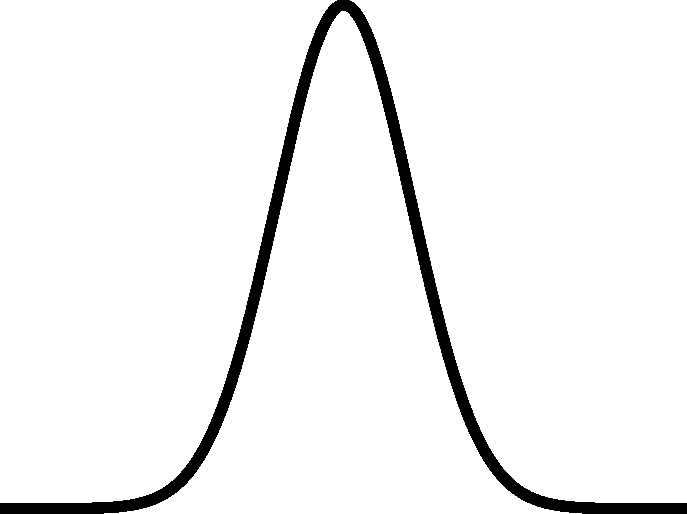
\includegraphics[width=0.5cm]{img/gaussian.pdf}};
				\node [comp, below = 0.5 of b] (c) {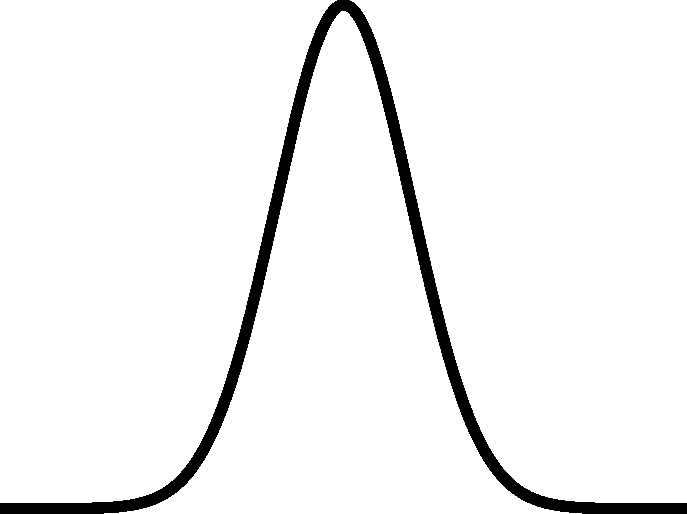
\includegraphics[width=0.5cm]{img/gaussian.pdf}};
				\coordinate [left = 1 of a, label = left:{\(x_1\)}] (A);
				\coordinate [left = 1 of b, label = left:{\(x_2\)}] (B);
				\coordinate [left = 1 of c, label = left:{\(x_3\)}] (C);
				\node [comp, right = 1 of b] (d) {\( \bigtimes \)};
				\coordinate [right = 1 of d, label = right:{\( p(x_1, x_2, x_3) = p(x_1) \, p(x_2) \, p(x_3) \)}] (D);
				\draw (A) to (a);
				\draw (B) to (b);
				\draw (C) to (c);
				\draw (a) to (d);
				\draw (b) to (d);
				\draw (c) to (d);
				\draw (d) to (D);
			\end{tikzpicture}
		\end{center}
		for three random variables. More random variables are denoted analogous. One example application for this is to model a multivariate Gaussian with diagonal covariance matrix. To represent mixture models over a single random variable, weighted sums are used. These are denoted as
		\begin{center}
			\begin{tikzpicture}[->, comp/.style = { draw, circle, minimum width = 0.75cm, minimum height = 0.75cm, inner sep = 0 }]
				\node [comp] (a) {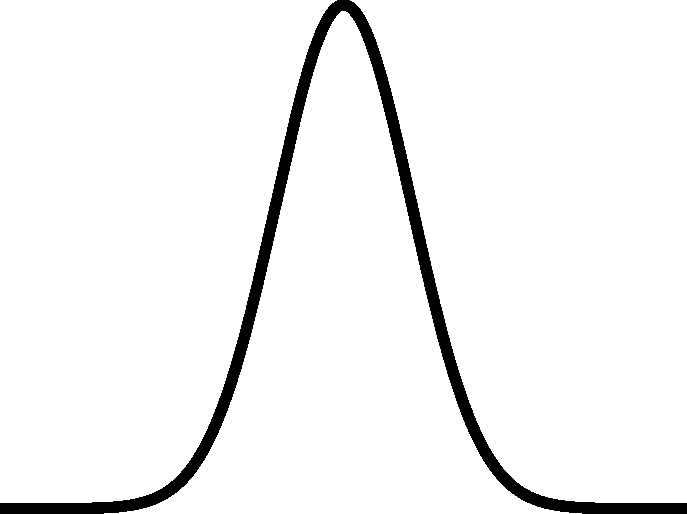
\includegraphics[width=0.5cm]{img/gaussian.pdf}};
				\node [comp, below = 0.5 of a] (b) {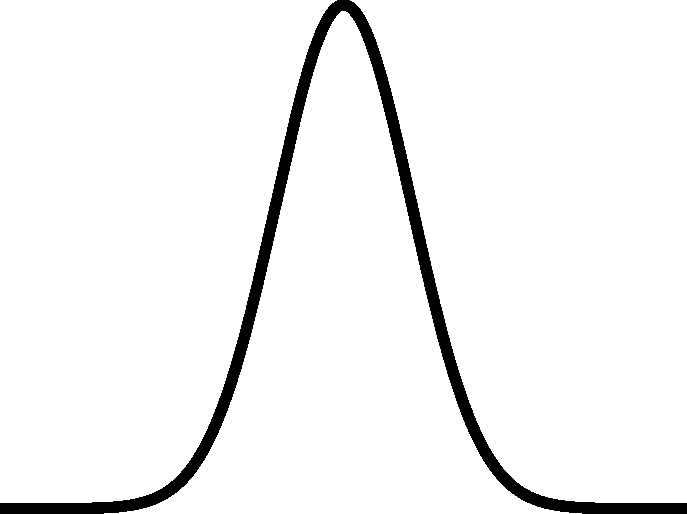
\includegraphics[width=0.5cm]{img/gaussian.pdf}};
				\node [comp, below = 0.5 of b] (c) {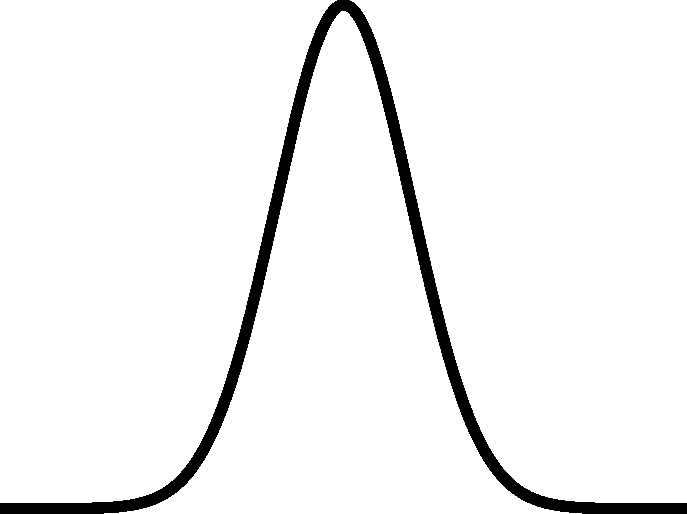
\includegraphics[width=0.5cm]{img/gaussian.pdf}};
				\coordinate [left = 1 of a, label = left:{\(x\)}] (A);
				\coordinate [left = 1 of b, label = left:{\(x\)}] (B);
				\coordinate [left = 1 of c, label = left:{\(x\)}] (C);
				\node [comp, right = 1 of b] (d) {\resizebox{0.5cm}{!}{\(+\)}};
				\coordinate [right = 1 of d, label = right:{\( p(x) = w_1 p(x) + w_2 p(x) + w_3 p(x) \)}] (D);
				\draw (A) to (a);
				\draw (B) to (b);
				\draw (C) to (c);
				\draw (a) to node[above, near start, xshift = +2pt]{\(w_1\)} (d);
				\draw (b) to node[above, near start, yshift = -2pt]{\(w_2\)} (d);
				\draw (c) to node[below, near start, xshift = +2pt, yshift = -2pt]{\(w_3\)} (d);
				\draw (d) to (D);
			\end{tikzpicture}
		\end{center}
		where the weights are written on the edges from the univariate distributions to the summing node. By stacking all these different nodes, expressive efficiency can be increased. It is, however, not possible to arbitrarily stack sums, products and distributions, certain structural constraints have to be fulfilled to ensure tractability. These will be covered in \autoref{subsec:probCircTractability}.

		But probabilistic circuits are not PGMs! They are probabilistic and graphical, but the nodes represent computations, not random variables and the edges determine the order of execution and do not encode dependencies. In PGMs, inference is done using conditioning, elimination, and message passing while in probabilistic circuits inference is done using forward- and backward-passes. So they are more like neural networks than PGMs. Due to them being computational graphs, a lot of things are possible: repeated computations can be cached, the operational semantics are clear and tractable in terms of circuit size, and they are differentiable, so gradient-based optimization is possible.

		\subsection{Ensuring Tractability}
			\label{subsec:probCircTractability}

			In order to ensure tractability in a probabilistic circuit, certain constraints have to be fulfilled. The first two obvious ones are \emph{decomposability} and \emph{smoothness}:
			\begin{description}
				\item[Decomposability] All product nodes have to be decomposable. A product node is decomposable if its children depend on a disjoint set of variables, i.e., the same variable does not appear twice on the incoming nodes.
				\item[Smoothness] All sum nodes have to be smooth. A sum node is smooth if its children depend on the same variable sets, i.e., the same variable has to be present on all incoming nodes.
			\end{description}
			These two properties enable tractable MAR and CON queries! This is due to large integrals that can be decomposed into easier ones
			\begin{equation}
				p(\vec{x}, \vec{y}) = p(\vec{x}) \, p(\vec{y})
				\quad\implies\quad
				\iint\! p(\vec{x}, \vec{y}) \dd{\vec{x}} \dd{\vec{y}}
					= \iint\! p(\vec{x}) \, p(\vec{y}) \dd{\vec{x}} \dd{\vec{y}}
					= \bigg(\! \int\! p(\vec{x}) \dd{\vec{x}} \!\!\bigg) \bigg(\! \int\! p(\vec{y}) \dd{\vec{y}} \!\!\bigg)
			\end{equation}
			and the marginalization sums can be pulled out of the integrals
			\begin{equation}
				p(\vec{x}) = \sum_i w_i p_i(\vec{x})
				\quad\implies\quad
				\int\! p(\vec{x}) \dd{\vec{x}}
					= \int \sum_i w_i p_i(\vec{x}) \dd{\vec{x}}
					= \sum_i w_i \int\! p_i(\vec{x}) \dd{\vec{x}}
			\end{equation}
			pushing the integrals down to the children. On both these cases, pre premise follows from the decomposability and smoothness property, respectively. To compute for example \( p(X_2, X_3) \) when there are four random variables, the inputs for \( X_1 \) and \( X_4 \) are set to \num{1} (as they get integrated out) and the inputs for \( X_2 \) and \( X_3 \) are set to their respective probability which is provided from the unimodal distribution.

			The next property that has to be ensured is \emph{determinism} (also known as \emph{selectivity}):
			\begin{description}
				\item[Determinism] All sum nodes have to be deterministic. A sum node is deterministic if the output of at most one children is non-zero for any input, e.g. if their distributions have disjoint support.
			\end{description}
			This property enables tractable MAP queries! This is due to the argmax on a mixture model that gets drastically simplified because the sum over the weights can be discarded. Let \( \vec{q} = \{ \vec{q}_x, \vec{q}_y \} \) and \( \vec{e} = \{ \vec{e}_x, \vec{e}_y \} \) be separated into two arbitrary sets of random variables, then from decomposability is follows that \( p(\vec{q}, \vec{e}) = p(\vec{q}_x, \vec{e}_x, \vec{q}_y, \vec{e}_y) = p(\vec{q}_x, \vec{e}_x) \, p(\vec{q}_y, \vec{e}_y) \). Thus, the argmax can be split at the product notes:
			\begin{equation}
				\arg\max_{\vec{q}} \; p(\vec{q} \given \vec{e})
					= \arg\max_{\vec{q}} \; p(\vec{q}, \vec{e})
					= \arg\max_{\vec{q}_x, \vec{q}_y} \; p(\vec{q}_x, \vec{e}_x, \vec{q}_y, \vec{e}_y)
					= \arg\max_{\vec{q}_x} \; p(\vec{q}_x, \vec{e}_x),\, \arg\max_{\vec{q}_y} \; p(\vec{q}_y, \vec{e}_y)
			\end{equation}
			and the optimizations can be solved separately. Due to determinism, i.e.
			\begin{equation}
				p(\vec{q}, \vec{e}) = \sum_i w_i p_i(\vec{q}, \vec{e}) = w_c p_c(\vec{q}, \vec{e})
			\end{equation}
			where \(p_i\) is the only non-zero distribution, the argmax of a sum node is extremely simple:
			\begin{equation}
				\arg\max_{\vec{q}} \; p(\vec{q}, \vec{e})
					= \arg\max_{\vec{q}} \; \sum_i w_i p_i(\vec{q}, \vec{e})
					= \arg\max_{\vec{q}} \; w_c p_c(\vec{q}, \vec{e})
			\end{equation}
			This pushes the argmax to the children. By repeatedly applying these two rules, the argmax can be pushed to the leaves (the random variables) where a MAP query is simple to answer as the mode of the unimodal distribution. In practice, the evaluation of a MAP query goes as follows:
			\begin{enumerate}
				\item Turn all sum nodes into (weighted) max nodes.
				\item Evaluate \( p(\vec{e}) \), the marginal of the given evidence, in a forward pass.
				\item Retrieve the max activations in a backward pass.
				\item Compute MAP queries at the leaves.
			\end{enumerate}
			Compares to MAR and CON queries, the computation has to be run two times through the network, but it is still linear in circuit size. If the circuit is non-deterministic, MAP is intractable, but the algorithm can still be used as an approximation. The circuit is then called a \emph{sum-product network} (SPN) which are equivalent the exception of determinism.

			The final requirement is \emph{structured decomposability}:
			\begin{description}
				\item[Structured Decomposability] A product node is structured decomposable if it decomposes according to a node in a binary tree.
			\end{description}
			This is a stronger requirement than decomposability and is not necessary for MAR, CON, and MAP queries. But it enables tractability of the \emph{entropy} of the circuit, \emph{symmetric} and \emph{group queries} (exactly \(k\), odd number, more, etc.), and, for the "right" binary tree, also the probability of logical circuit event in a probabilistic circuit, \emph{multiplication} of two probabilistic circuits, \emph{KL-divergence} between two circuits, \emph{same-decision probability}, \emph{expected same-decision probability}, \emph{expected classifier agreement}, and \emph{expected predictions}. But as structure decomposability is a pretty harsh requirement, it is usually not enforced.
		% end

		\subsection{Other Circuits and Circuit Compilation}
			This section addresses the similarities and differences between probabilistic, logical, and other circuits. The tractable probabilistic inference view exploits efficient summation for decomposable functions in the commutative semi-ring of probabilities, \( (\R, +, \times, 0, 1) \). This is also possible in other semi-rings with generalized operations, \( (\mathbb{S}, \oplus, \otimes, 0_\oplus, 1_\otimes) \). Historically a very well studied semi-ring is the one for boolean functions: \( (\mathbb{B} = \{ 0, 1 \}, \lor, \land, 0, 1) \). These lead to logical circuits which represent logical functions in a compact way. These look the same way as probabilistic circuits, but the nodes are logical ands and ors instead of sums and products. Also similar to probabilistic circuits, it is possible to define structural properties like \emph{decomposability}, \emph{smoothness}, and \emph{determinism} to allow for tractable computations and---in some sense---inference of boolean values.

			% TODO: PGMs: Weighted Model Counting; 10b.109

			\subsubsection{Circuit Compilation: From Trees to Circuits}
				A big step into tractability is to compile probabilistic graphical models---or probabilistic trees only, in this section---into probabilistic circuits. This can be done in a bottom-up approach: at first a leaf node of the probabilistic tree is compiled into a sum node structure in the probabilistic circuit where for each value of the leaf there exists one leaf in the circuit and for each value of the dependent variable there exists a sum node. The weights are the probabilities. This is done for every leaf node of the tree. Then these structures are taken as leaves with multiple outputs, corresponding to each value of the random variables. The "leaf structures" are then used to recursively build up the parent nodes of the probabilistic tree which builds up the circuit in the end.

				Take, for example, the probabilistic tree shown in \autoref{fig:probTree}. To compile the first node, the probabilities
				\begin{align}
					P(A = 0 \given C = 0) &= 0.3 &
					P(A = 1 \given C = 0) &= 0.7 \\
					P(A = 0 \given C = 1) &= 0.6 &
					P(A = 1 \given C = 1) &= 0.4
				\end{align}
				are used. First the circuit for \( P(A \given C = 0) \) is built and subsequently the circuit for \( P(A \given C = 1) \) is added. Both of these steps are shown in \autoref{fig:probTreeCirc1a} and \ref{fig:probTreeCirc1a}. Analogously the circuit for \( P(B \given C = 0/1) \) is built in \autoref{fig:probTreeCirc1c} and \ref{fig:probTreeCirc1d}. To now build the probabilities \(P(A, B, C = 0/1)\) and \(P(A, B, C)\), the already build probabilities have to be multiplied and then \(C\) has to be summed up w.r.t. the probabilities \( P(C = 0) = 0.2 \) and \( P(C = 1) = 0.8 \). All of this is shown in \autoref{fig:probTreeCirc1e}.

				\begin{figure}
					\centering
					\begin{tikzpicture}[->, rv/.style = { draw, circle, minimum width = 1cm, minimum height = 1cm, inner sep = 0 }]
						\node [rv] (c) {\(C\)};
						\node [rv, below = 1 of c, xshift = -1cm] (b) {\(B\)};
						\node [rv, below = 1 of c, xshift = +1cm] (a) {\(A\)};
						\draw (c) to (b);
						\draw (c) to (a);
					\end{tikzpicture}
					\caption{Example probabilistic tree.}
					\label{fig:probTree}
				\end{figure}

				\begin{figure}
					\centering
					\begin{subfigure}{0.35\linewidth}
						\centering
						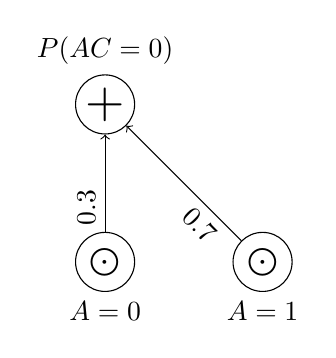
\begin{tikzpicture}[->, xscale = 2, yscale = 2, comp/.style = { draw, circle, minimum width = 0.75cm, minimum height = 0.75cm, inner sep = 0 }]
							\node [comp, label = below:{\( A = 0 \)}] (A0) at (0, 0) {\(\bigodot\)};
							\node [comp, label = below:{\( A = 1 \)}] (A1) at (1, 0) {\(\bigodot\)};
							\node [comp, label = above:{\( P(A \given C = 0) \)}] (AgivenC0) at (0, 1) {\resizebox{0.5cm}{!}{\(+\)}};

							\draw (A0) to node[above, sloped, near start]{\(0.3\)} (AgivenC0);
							\draw (A1) to node[below, sloped, near start]{\(0.7\)} (AgivenC0);
						\end{tikzpicture}
						\caption{Compilation of \( P(A \given C = 0) \).}
						\label{fig:probTreeCirc1a}
					\end{subfigure}
					~
					\begin{subfigure}{0.35\linewidth}
						\centering
						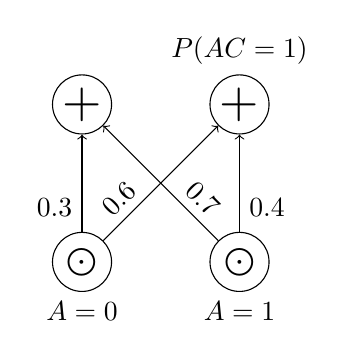
\begin{tikzpicture}[->, xscale = 2, yscale = 2, comp/.style = { draw, circle, minimum width = 0.75cm, minimum height = 0.75cm, inner sep = 0 }]
							\node [comp, label = below:{\( A = 0 \)}] (A0) at (0, 0) {\(\bigodot\)};
							\node [comp, label = below:{\( A = 1 \)}] (A1) at (1, 0) {\(\bigodot\)};
							\node [comp] (AgivenC0) at (0, 1) {\resizebox{0.5cm}{!}{\(+\)}};
							\node [comp, label = above:{\( P(A \given C = 1) \)}] (AgivenC1) at (1, 1) {\resizebox{0.5cm}{!}{\(+\)}};

							\draw (A0) to node[left,  near start]{\(0.3\)} (AgivenC0);
							\draw (A1) to node[above, sloped, near start]{\(0.7\)} (AgivenC0);
							\draw (A0) to node[above, sloped, near start]{\(0.6\)} (AgivenC1);
							\draw (A1) to node[right, near start]{\(0.4\)} (AgivenC1);
						\end{tikzpicture}
						\caption{Compilation of \( P(A \given C = 1) \).}
						\label{fig:probTreeCirc1b}
					\end{subfigure} \\ \vspace{0.4cm}
					\begin{subfigure}{0.35\linewidth}
					\centering
						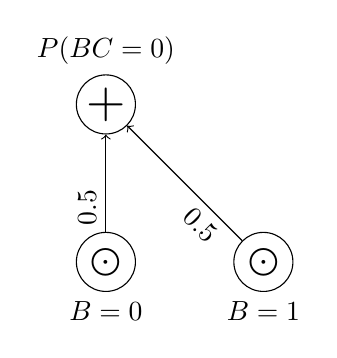
\begin{tikzpicture}[->, xscale = 2, yscale = 2, comp/.style = { draw, circle, minimum width = 0.75cm, minimum height = 0.75cm, inner sep = 0 }]
							\node [comp, label = below:{\( B = 0 \)}] (B0) at (0, 0) {\(\bigodot\)};
							\node [comp, label = below:{\( B = 1 \)}] (B1) at (1, 0) {\(\bigodot\)};
							\node [comp, label = above:{\( P(B \given C = 0) \)}] (BgivenC0) at (0, 1) {\resizebox{0.5cm}{!}{\(+\)}};

							\draw (B0) to node[above, sloped, near start]{\(0.5\)} (BgivenC0);
							\draw (B1) to node[below, sloped, near start]{\(0.5\)} (BgivenC0);
						\end{tikzpicture}
						\caption{Compilation of \( P(B \given C = 0) \).}
						\label{fig:probTreeCirc1c}
					\end{subfigure}
					~
					\begin{subfigure}{0.35\linewidth}
						\centering
						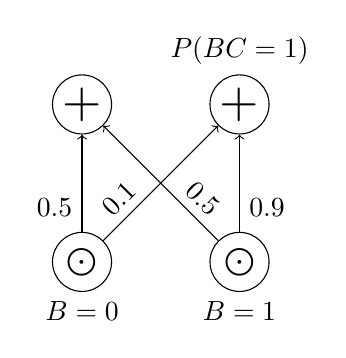
\begin{tikzpicture}[->, xscale = 2, yscale = 2, comp/.style = { draw, circle, minimum width = 0.75cm, minimum height = 0.75cm, inner sep = 0 }]
							\node [comp, label = below:{\( B = 0 \)}] (B0) at (0, 0) {\(\bigodot\)};
							\node [comp, label = below:{\( B = 1 \)}] (B1) at (1, 0) {\(\bigodot\)};
							\node [comp] (BgivenC0) at (0, 1) {\resizebox{0.5cm}{!}{\(+\)}};
							\node [comp, label = above:{\( P(B \given C = 1) \)}] (BgivenC1) at (1, 1) {\resizebox{0.5cm}{!}{\(+\)}};

							\draw (B0) to node[left,  near start]{\(0.5\)} (BgivenC0);
							\draw (B1) to node[above, sloped, near start]{\(0.5\)} (BgivenC0);
							\draw (B0) to node[above, sloped, near start]{\(0.1\)} (BgivenC1);
							\draw (B1) to node[right, near start]{\(0.9\)} (BgivenC1);
						\end{tikzpicture}
						\caption{Compilation of \( P(B \given C = 1) \).}
						\label{fig:probTreeCirc1d}
					\end{subfigure} \\ \vspace{0.4cm}
					\begin{subfigure}{0.7\linewidth}
						\centering
						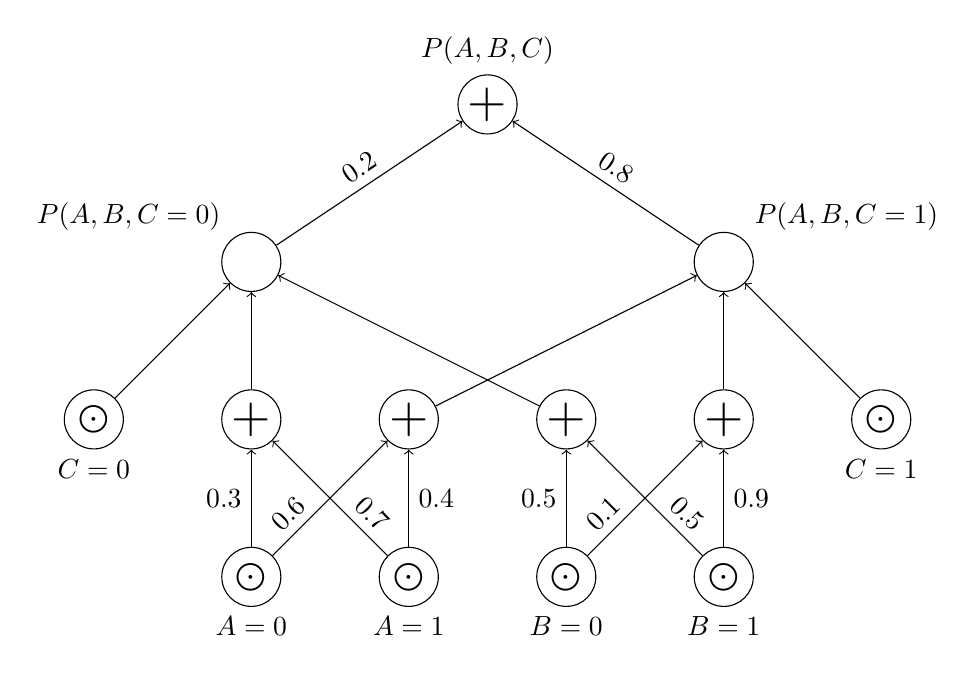
\begin{tikzpicture}[->, xscale = 2, yscale = 2, comp/.style = { draw, circle, minimum width = 0.75cm, minimum height = 0.75cm, inner sep = 0 }]
							\node [comp, label = below:{\( A = 0 \)}] (A0) at (0, 0) {\(\bigodot\)};
							\node [comp, label = below:{\( A = 1 \)}] (A1) at (1, 0) {\(\bigodot\)};
							\node [comp] (AgivenC0) at (0, 1) {\resizebox{0.5cm}{!}{\(+\)}};
							\node [comp, label] (AgivenC1) at (1, 1) {\resizebox{0.5cm}{!}{\(+\)}};

							\node [comp, label = below:{\( B = 0 \)}] (B0) at (2, 0) {\(\bigodot\)};
							\node [comp, label = below:{\( B = 1 \)}] (B1) at (3, 0) {\(\bigodot\)};
							\node [comp] (BgivenC0) at (2, 1) {\resizebox{0.5cm}{!}{\(+\)}};
							\node [comp, label] (BgivenC1) at (3, 1) {\resizebox{0.5cm}{!}{\(+\)}};

							\node [comp, label = below:{\( C = 0 \)}] (C0) at (-1, 1) {\(\bigodot\)};
							\node [comp, label = above left:{\( P(A, B, C = 0) \)}] (ABC0) at (0, 2) {\(\bigtimes\)};

							\node [comp, label = below:{\( C = 1 \)}] (C1) at (4, 1) {\(\bigodot\)};
							\node [comp, label = above right:{\( P(A, B, C = 1) \)}] (ABC1) at (3, 2) {\(\bigtimes\)};

							\node [comp, label = above:{\( P(A, B, C) \)}] (ABC) at (1.5, 3) {\resizebox{0.5cm}{!}{\(+\)}};

							\draw (A0) to node[left]{\(0.3\)} (AgivenC0);
							\draw (A1) to node[above, sloped, near start]{\(0.7\)} (AgivenC0);
							\draw (A0) to node[above, sloped, near start]{\(0.6\)} (AgivenC1);
							\draw (A1) to node[right]{\(0.4\)} (AgivenC1);

							\draw (B0) to node[left]{\(0.5\)} (BgivenC0);
							\draw (B1) to node[above, sloped, near start]{\(0.5\)} (BgivenC0);
							\draw (B0) to node[above, sloped, near start]{\(0.1\)} (BgivenC1);
							\draw (B1) to node[right]{\(0.9\)} (BgivenC1);

							\draw (C0) to (ABC0);
							\draw (AgivenC0) to (ABC0);
							\draw (BgivenC0) to (ABC0);
							\draw (C1) to (ABC1);
							\draw (AgivenC1) to (ABC1);
							\draw (BgivenC1) to (ABC1);

							\draw (ABC0) to node[above, sloped]{\(0.2\)} (ABC);
							\draw (ABC1) to node[above, sloped]{\(0.8\)} (ABC);
						\end{tikzpicture}
						\caption{}
						\label{fig:probTreeCirc1e}
					\end{subfigure}
					\caption{Steps of compiling the probabilistic tree in \autoref{fig:probTree} into a probabilistic circuit. The distribution node with a \(\odot\) described the binary distribution that outputs \num{0} if the condition below the node holds and \num{1} otherwise. Hence, the nodes \( A = 0 \) and \( A = 1 \) are mutually exclusive and determinism holds (similar for the others).}
					\label{fig:probTreeCirc1}
				\end{figure}
			% end

			\subsubsection{Equivalent and Related Formulations}
				As trees, polytrees and thin junction trees can be turned into decomposable, smooth, and deterministic probabilistic circuits, they all support tractable EVI, MAR, CON, and MAP queries. The same goes for arithmetic circuits (ACs) which are also decomposable, smooth, and deterministic.

				Other equivalent formulations are:
				\begin{itemize}
					\item \emph{Cutset networks} (CNets): CNets are weighted decision trees whose leaves are Bayesian networks. It is possible to replace every decision node by a deterministic and smooth sum node, and thus it is possible to compile CNets into probabilistic circuits. Hence, they are decomposable, smooth, and deterministic and thus EVI, MAR, CON, and MAP queries are tractable.
					\item \emph{Probabilistic sentential decision diagrams} (PSDDs): These are also \emph{structured} decomposable, smooth, and deterministic. Hence, EVI, MAR, CON, MAP, and also complex queries are tractable!
				\end{itemize}
				As probabilistic circuits are so diverse and expressive, they belong to the most expressive while still tractable models!
			% end
		% end
	% end

	\section{Building Circuits} % 10a.39
		After discussing probabilistic circuits and seeing how expressive and expression efficient they are, the next big question is how to build these circuits tractably because usually the circuits are not given but the shall be learned from data. The first step is to define a \emph{tractable learner}: a learner \(L\) is \emph{tractable} for a class of queries \(\mathcal{Q}\) if and only if
		\begin{enumerate}
			\item for any dataset \(\mathcal{D}\), the learner \( L(\mathcal{D}) \) runs in \( \mathcal{O}\big( \mathrm{poly}(\lvert \mathcal{D} \rvert) \big) \). This guarantees that the size of the learned model is in \( \mathcal{O}\big( \mathrm{poly}(\lvert \mathcal{D} \rvert) \big) \cap \mathcal{O}\big( \mathrm{poly}(\lvert \vec{X} \rvert) \big) \).
			\item it outputs a probabilistic model that is tractable for all queries in the class \(\mathcal{Q}\). This guarantees efficient querying for \(\mathcal{Q}\) in time \( \mathcal{O}\big( \mathrm{poly}(\lvert \vec{X} \rvert) \big) \).
		\end{enumerate}
		This section will now introduce different methods for learning circuit parameters and also structure. Additionally, compilation of other models into circuits is covered.

		\subsection{Learning Circuit Parameters}
			The easiest part of circuit learning is learning the parameters, i.e. the probabilities, of the circuit. These are leaf parameters \(\vec{\theta}\) and the weights \(\vec{w}\) on summing nodes. For deterministic circuits, this can be done in closed form with convex optimization. For non-deterministic circuits, this is harder. Some algorithms for learning the parameters in non-deterministic circuits are SGD, soft/hard EM, Bayesian moment matching, collapsed variational Bayes, CCCP, and extended Baum-Welch. This section will covert the former two algorithms.

			\subsubsection{Deterministic Circuits}
				For deterministic circuits, approximating the parameters can simply be done by maximizing the data likelihood
				\begin{equation}
					\vec{\theta}^\mathrm{MLE}, \vec{w}^\mathrm{MLE}
						= \arg\max_{\vec{\theta}, \vec{w}} \; L(\vec{\theta}, \vec{w}; \mathcal{D})
						= \arg\max_{\vec{\theta}, \vec{w}} \; \prod_{d \in \mathcal{D}} p_{\vec{\theta}, \vec{w}}(d).
				\end{equation}
				With determinism, the likelihood decomposes over the parameters and the optimization problem has a closed-form solution.
			% end

			\subsubsection{Hard/Soft Parameter Updating: Gradient Descent and EM}
				Optimizing the parameters via gradient descent is simply done by computing the gradient of the likelihood and applying standard optimization techniques. For using EM, each summing node is considered as the marginalization over a hidden variable that is estimated in the E-step.
			% end

			\subsubsection{Bayesian Parameter Learning}
				In \emph{Bayesian} parameter learning, a prior \( p(\vec{w}) \) is put on the weights of the circuit. Then the posterior
				\begin{equation}
					p(\vec{w} \given \mathcal{D}) \propto p(\mathcal{D} \given \vec{w}) \, p(\vec{w})
				\end{equation}
				is maximized. But this posterior is intractable! Instead of a general prior, a factorized prior
				\begin{equation}
					p(\vec{w}) = \prod_{i \in \text{Sum Nodes}} \mathit{Dir}(\vec{w}_i \given \alpha_i)
				\end{equation}
				is assumed in a circuit with normalized weights \( w_{ij} \geq 0 \) and \( \sum_j w_{ij} = 1 \) where \( i \in \text{Sum Nodes} \). The posterior then becomes a mixture of Dirichlet distributions where the number of mixture components is exponential in the number of sum nodes.

				\paragraph{Moment Matching (oBMM)}
					The posterior is approximated with a tractable distribution after each update that matches some moments of the exact, but intractable, posterior. The joint \(p(\vec{w})\) is approximated by a product of Dirichlet distributions and the first and second moment of each marginal \(p(\vec{w}_i)\) are used to set the parameters \(\alpha_i\) of each Dirichlet.
				% end

				\paragraph{oBMM Extended}
					Uses continuous models with Gaussian leavers.
				% end

				\paragraph{CVB-SPN}
					Uses a collapsed variational inference algorithm and produces better results than oBMM.
				% end

				\paragraph{Sequential Monomial Approximation and Concave-Convex Procedure}
					Any complete and decomposable circuit can be transformed into a mixture of trees where each tree corresponds to a product of univariate distributions. \emph{Sequential monomial approximation} learns the parameters based on a maximum likelihood estimator which can be formulated as a sigmonial program. This program can equivalently be transformed into a different of convex functions, yielding the \emph{concave-convex procedure}.
				% end
			% end
		% end

		\subsection{Structure Learning}
			Instead of "just" learning the parameters of a probabilistic circuit, \emph{structure learning} algorithms address the problem of learning the structure of the circuit, i.e., the connections between the nodes.

			A general approach for learning the structure is to start with a dense circuit and then find the structure by learning the weights and removing connections with near-zero weights. This is, in principle, possible to every arithmetic circuit by implementing it in any autograd library. It also works well but there are more advanced algorithms that produce better results.

			\paragraph{LearnSPN and Variants}
				\emph{LearnSPN} learns both structure and parameters of a circuit simultaneously. For this it starts from a data matrix that lists all values for each random variable. Then clusters are searched in the data for building sum nodes. Once clusters have been found and sum nodes have been created, an independence test is used within the leaves to find independent random variables. Once these have been found, the circuit is factorized into these random variables. These two steps iterate until either no clusters can be found anymore.

				A variant of LearnSPN is ID-SPN which starts with a single arithmetic circuit (AC) that represents a tractable Markov network. The process of clustering instances and variables for sum and product nodes is then stopped before the process reaches univariate distributions. These are replaced by a learned tractable MN represented by an AC factorizing multiple distributions. This creates an SPN with tractable multivariate distributions as leaves, so-called Markov network arithmetic circuits (MN AC).

				Another variant is \emph{bottom-up learning} which start from a simple model over a small variable scope and increase this model successively over a larger variable scope guided by dependence tests and a maximum mutual information principle. Other variants are \emph{greedy for deterministic circuits} and \emph{graph SPNs} which transform the network as a hill climbing algorithm using split and merge operations and form tree SPNs my merging similar sub-structures, respectively.
			% end

			% TODO: PGMs: Building Circuits: Structure Learning; 10b.150--10b.160, 10b.161--19b.162, 10b.166--10b.168

%			\paragraph{Cut(e)set Network}
%				\emph{Cut(e)set networks} use likelihood decompositions for learning the parameters and for structure learning start with a single tractable model and substitute leaf nodes with the best CNet which improves all likelihood decompositions.
%			% end
%
%			\paragraph{PSDD Structure Learning}
%				\emph{PSDD structure learning} learning a binary tree where the leaves are labeled with variables and the internal nodes split the variables into those appearing in the left and those appearing in the right sub-tree. Learning takes place in a bottom-up or top-down fashion max maximizing the pairwise MI instead of the joint MI.
%			% end
%
%			\paragraph{LearnPSDD}
%				\emph{LearnPSDD} incrementally improves the structure of a PSDD to better fit the data. Learning continuous until the log-likelihood on the validation data set converges or a desired time or size limit is reached. In every step the structure is changed by executing an operation that is greedily chosen based on the best likelihood improvement per size increment.
%			% end
%
%			\paragraph{Learning Logic Circuits}
%				To learn logic circuits, the values and parameters are propagated bottom-up. For parameter learning, due to decomposability and determinism, any logic circuit model can be reduced to a logistic regression model over some features. For structure learning, split operations like in LearnPSDD are performed.
%			% end

%			\paragraph{Bayesian Structure Learning} % 10b.156
%				\todo{Content}
%			% end
%
%			\paragraph{Automatic Bayesian Density Analysis (ABDA)} % 10b.157, 10b.158
%				\todo{Content}
%			% end
%
%			\paragraph{Bayesian SPNs} % 10b.159, 10b.160
%				\todo{Content}
%			% end
%
%			\paragraph{Randomized Structure Learning: RAT-SPNs} % 10b.161, 19b.162
%				\todo{Content}
%			% end
%
%			\paragraph{Extremely Randomized CNets: XCNets} % 10b.166, 10b.167
%				\todo{Content}
%			% end
%
%			\paragraph{Online Learning} % 10b.168
%				\todo{Content}
%			% end
		% end

		\subsection{Ensembles of Probabilistic Circuits}
			To solve issues like the tendency of overfitting of probabilistic circuits and to improve accuracy of a single model, probabilistic circuits an be used in an ensemble in the form of a mixture model
			\begin{equation}
				p(\vec{x}) = \sum_{i = 1}^{K} \lambda_i C_i(\vec{x}),\quad \lambda_i \geq 0, \sum_{i = 1}^{K} \lambda_1 = 1.
			\end{equation}
			To learn both the parameters of each circuit and to learn the mixture components weights \(\vec{\lambda}\), an EM-algorithm can be employed. But this raises some issues in convergence and stability, making this impractical.

			A better alternative for using circuit ensembles is bagging which is more efficient than EM. For training the circuits the mixture components are all set equally probable and are then learned independently on different bootstraps. To make these models even more efficient, random subspace projects can be added (like for CNets).

			It is also possible to boost probabilistic circuits. One method the \emph{boosting density estimation} (BDE) which works like AdaBoost and combined models in the form \( f_m = (1 - \eta_m) f_{m - 1} + \eta_m c_m \) where \(f_m\) is the \(m\)-th model, \(c_m\) is the current weak learner and \(\eta_m\) is the weight of that learner. Another method is GBDE which is kernel-based. It is also possible to use sequential EM which jointly optimized \(\eta_m\) and \(c_m\) while keeping \(f_{m - 1}\) fixed.
		% end

		% TODO: PGMs: Building Circuits: Knowledge Compilation; 10b.169, 10b.170, 10b.171, 10b.172, 10b.173
	% end

	\section{Applications}
		This sections shows some of the applications of tractable inference and probabilistic graphical models in general.

		% TODO: PGMs: Applications; 10a.4, 10a.5, 10b.174--10b.190

%		\paragraph{Computer Vision} % 10b.178, 10a.5
%			\todo{Content}
%		% end
%
%		\paragraph{Image Segmentation} % 10b.179
%			\todo{Content}
%		% end
%
%		\paragraph{Scene Understanding: Su-PAIR} % 10b.180
%			\todo{Content}
%		% end
%
%		\paragraph{Activity Recognition} % 10b.182
%			\todo{Content}
%		% end
%
%		\paragraph{Speec Reconstriction and Extension} % 10b.183, 10a.4
%			\todo{Content}
%		% end
%
%		\paragraph{Sequence Labeling} % 10b.184
%			\todo{Content}
%		% end
%
%		\paragraph{Robotics} % 10b.185
%			\todo{Content}
%		% end
%
%		\paragraph{SOP: Preference Learning} % 10b.186
%			\todo{Content}
%		% end
%
%		\paragraph{SOP: Routing} % 10b.187
%			\todo{Content}
%		% end
%
%		\paragraph{Probabilistic Programming} % 10b.189
%			\todo{Content}
%		% end
%
%		\paragraph{And more\dots} % 10b.190
%			\todo{Content}
%		% end
	% end

	\section{Takeaways and Open Challenges}
		The three primary challenges in probabilistic graphical models are:
		\begin{enumerate}
			\item \emph{Better benchmarks:} \\
				To move beyond toy problems and dataset reflecting to complex and heterogeneous nature of real data. Move towards fully automated reasoning!
			\item \emph{Hybridizing tractable and intractable models:} \\
				Use tractable models inside intractable loops and glue together small intractable boxed by tractable inference.
			\item \emph{Scaling tractable learning:} \\
				Learn tractable models with millions of datapoints and thousands of feature in tractable time.
		\end{enumerate}
		The takeaways are that tractability is a spectrum and there are more and less tractable models, it is possible to be both tractable and expressive at the same time (probabilistic circuits), probabilistic circuits are the foundation for tractable inference and learning, and that there is still a lot more to do.
	% end
% end

\chapter{Natural Language Processing}
	\emph{Natural language processing} (NLP) is concerned with processing, interpreting, and translating naturally spoken or written text. This chapter will cover some parts of natural language understanding in form of the underlying semantics (\autoref{sec:textSemantics}) as well as translation and structure extraction (\autoref{sec:translation}).

	\section{Text Semantics}
		\label{sec:textSemantics}

		In NLP, \emph{text semantics} addresses the problem of extracting the meaning of texts. The models in this category can be split into two supercategories:
		\begin{description}[leftmargin = 5cm]
			\item[Propositional Semantics]
				Text gets translated into a logical language, e.g. predicate calculus. For example the text "dog bites man" can be translated into the formula \( \mathrm{bites}(\mathrm{dog}, \mathrm{man}) \), where \( \mathrm{bites}(\cdot, \cdot) \) is a binary relation and \(\mathrm{man}\) and \(\mathrm{dog}\) are objects. It is also possible to attach probabilities to these formulas.
			\item[Vector Representation]
				Text is embedded into a high-dimensional vector space. For example the text "dog bites man" can be represented as a vector \( (0.2, -0.3, 1.5, \,\cdots\!) \in \R^n \). Sentences with a similar meaning should then be close to this embedding.
		\end{description}
		Text semantics can again be decomposed into two kinds of analysis: \emph{lexical} and \emph{compositional} semantics. In the former the meaning of individual words is analyzed while in the latter the meaning depends on the surrounding words and how they are combined. The next two sections will focus on propositional semantics and vector representations, respectively which can be used for both lexical and compositional semantics.

		\subsection{Propositional Semantics}
			Propositional semantics allow for logical inferences and allow the use of powerful result from logic to interpret text. For example: it is possible to infer "Socrates is mortal" from "Socrates is a man" and "all men are mortal".

			% TODO: NLP: Prop. Semantics; 11.12, 11.13, 11.14
			% TODO: NLP: Prop. Semantics: Contemporary Approaches; 11.6, 11.7, 11.8, 11.9, 11.10, 11.11
		% end

		\subsection{Vector Representation}
			The second approach to semantic analysis are vector embedding of words. These are based on a notion of \emph{similarity} and are based on the definition of paradigmatic similarity: similar words occur in similar contexts and are exchangeable. Word embeddings are vectors in a high dimensional vector space usually use a bag-of-words, for example:
			\begin{gather}
				\mathrm{vec}(\text{"dog"}) = \begin{bmatrix} 0.2 \\ -0.3 \\ 1.5 \\ \vdots \end{bmatrix} \qquad\qquad\quad
				\mathrm{vec}(\text{"bites"}) = \begin{bmatrix} 0.5 \\ 1.0 \\ -0.4 \\ \vdots \end{bmatrix} \qquad\qquad\quad
				\mathrm{vec}(\text{"man"}) = \begin{bmatrix} -0.1 \\ 2.3 \\ -1.5 \\ \vdots \end{bmatrix} \\
				\implies\qquad
				\mathrm{vec}(\text{"dog bites man"})
					= \mathrm{vec}(\text{"dog"}) + \mathrm{vec}(\text{"bites"}) + \mathrm{vec}(\text{"man"})
					= \begin{bmatrix} 0.6 \\ 2.0 \\ -0.4 \\ \vdots \end{bmatrix}
			\end{gather}
			The following sections will cover four models that all fall into the category of vector representations: latent semantic analysis, word2vec, skip-thought vectors and Siamese networks.

			\subsubsection{Latent Semantic Analysis}
				\emph{Latent semantic analysis} (LSA) uses a bag-of-words format for studying documents. All documents are encoded in a matrix \( \mat{T} \in \R^{N \times M} \) where the entry \(T_{ij}\) represents how often word \(j\) appears in document \(i\)\footnote{Where \(N\) and \(M\) are the total number of documents and words/word features, respectively.}. Often not the count is used as a metric but tf-idf (term frequency-inverse document frequency) or other "squashing" functions. Obviously, most entries of the matrix are zero. Then an approximate factorization \( \mat{T} \approx \mat{U}^T \mat{S} \mat{V} \) with \( \mat{U}^T \in \R^{N \times K} \), \( \mat{S} \in \R^{K \times K} \), \( \mat{V} \in \R^{K \times M} \) is computed where \(K\) is the latent dimensionality. If \(K = M\), then this is the singular value decomposition of \(\mat{T}\). The latent dimensionality \(\mat{K}\) is chosen based on the Eigenvalues of \(\mat{S}\) by leaving out the smallest Eigenvalues.

				Given a document \(\vec{t}\), i.e., a row of \(\mat{T}\), \( \vec{v} = \mat{V} \vec{t} \) is an embedding of the document in the latent space and \( \vec{t}' = \mat{U}^T \vec{v} = \mat{U}^T \mat{V} \vec{t} \) is the decoding from its embedding. The latent space can then be used to compute similarities between documents.

				Note how singular value decomposition of the term frequency matrix is used in order to compute the most relevant Eigenvectors for the embedding. This is similar to principal component analysis which essentially does the same thing, but on the covariance matrix. Also, as PCA first normalizes the data, it looses the sparseness of the factorized matrix, making it infeasible for large bag-of-words.
			% end

			\subsubsection{Word2Vec}
				As opposed to latent semantic analysis, \emph{word2vec} does not use entire documents but only a few positions before and after a word to determine its local context. The pairs of these words are called \emph{skip-grams}. For example, if three context words are used\footnote{Three to five words are usual.}, the {\color{TUDa-9b} red} word is the center word and the {\color{TUDa-1b} blue} words are the context words:
				\begin{center}
					"This is a sentence {\color{TUDa-1b} that does not} {\color{TUDa-9b} contain} {\color{TUDa-1b} any content and} can thus be ignored."
				\end{center}
				In a complete word2vec model, all words are considered as center words. The model is then trained for trying to predict the context words given a center word. It is also possible to train the inverse, i.e., predict the center word given context words, but skip-grams in general perform better. Training is done by optimizing a softmax loss
				\begin{equation}
					p(j \given i) = \frac{\exp\big\{ \vec{u}_j^T \vec{v}_i \big\}}{\sum_k \exp\big\{ \vec{u}_k^T \vec{v}_i \big\}}
				\end{equation}
				where \(j\) is the output word, \(i\) is the input word, and \(j\) ranges over the context (e.g. from \num{-3} to \num{+3} if three context words are used). The vectors \(\vec{u}_j\) and \(\vec{v}_i\) are output and input embedding vectors, respectively. Word2Vec can thus be implemented with standard deep learning tools by differentiating the loss to optimize the output and input embeddings.

				Compared to LSA, local contexts reveal much more information about relations and properties between words than LSA. Relations between words are characterized by their displacement, e.g. \( \mathrm{vec}(\text{"woman"}) - \mathrm{vec}(\text{"man"}) \) describes the distance between the word "woman" and the word "man". Word2Vec manages to generalize these structures, such that the said distance is for example roughly equal to the distance between "queen" and "king":
				\begin{equation}
					\mathrm{vec}(\text{"woman"}) - \mathrm{vec}(\text{"man"}) \approx \mathrm{vec}(\text{"queen"}) - \mathrm{vec}(\text{"king"})
				\end{equation}
				These kinds of relations can be found a lot when analyzing the results from word2vec models.
			% end

			\subsubsection{Skip-Thought Embeddings}
				All vector representation models discussed before only capture bag-of-words, i.e., the order of how words appear is neglected. But order matters! Take for example the two sentences "dog bites man" and "man bites dog": they have opposite meanings. \emph{Skip-though embeddings} use many-to-many RNNs for predicting the next and previous sentence. The hidden state after the complete sentence was entered into the RNN (but before the prediction started) is then used as the vector embedding. Once the RNN is trained, the two prediction heads can be discarded. \autopageref{fig:skipThoughtVector} illustrates this.

				\begin{figure}
					\centering
					\begin{tikzpicture}[
								->,
								label/.style = {
									text height = 0.3cm,
									inner sep = 0,
									minimum height = 0.4cm
								},
								input/.style = {
									fill = TUDa-0b,
									draw,
									circle,
									minimum width = 0.5cm,
									minimum height = 0.5cm,
									inner sep = 0
								},
								previous/.style = {
									fill = TUDa-4a,
									draw,
									circle,
									minimum width = 0.5cm,
									minimum height = 0.5cm,
									inner sep = 0
								},
								next/.style = {
									fill = TUDa-2a,
									draw,
									circle,
									minimum width = 0.5cm,
									minimum height = 0.5cm,
									inner sep = 0
								}
							]
						\node [input] (a) {};
						\node [input, right = 0.65 of a] (b) {};
						\node [input, right = 0.65 of b] (c) {};
						\node [input, right = 0.65 of c] (d) {};
						\node [input, right = 0.65 of d] (e) {};
						\node [input, right = 0.65 of e] (f) {};
						\node [input, right = 0.65 of f] (g) {};
						\node [input, right = 0.65 of g] (h) {};
						\node [input, right = 1.25 of h] (i) {};
						\node [draw, circle, dashed, minimum width = 1.25cm, minimum height = 1.25cm, inner sep = 0] at (i) {};

						\node [previous, above = 0.5 of i, xshift = 1.5cm] (pa) {};
						\node [previous, right = 0.65 of pa] (pb) {};
						\node [previous, right = 0.65 of pb] (pc) {};
						\node [previous, right = 0.65 of pc] (pd) {};
						\node [previous, right = 0.65 of pd] (pe) {};

						\node [next, below = 0.5 of i, xshift = 1.5cm] (na) {};
						\node [next, right = 0.65 of na] (nb) {};
						\node [next, right = 0.65 of nb] (nc) {};
						\node [next, right = 0.65 of nc] (nd) {};

						\draw (a) to (b);
						\draw (b) to (c);
						\draw (c) to (d);
						\draw (d) to (e);
						\draw (e) to (f);
						\draw (f) to (g);
						\draw (g) to (h);
						\draw (h) to (i);

						\draw (i) to (pa);
						\draw (pa) to (pb);
						\draw (pb) to (pc);
						\draw (pc) to (pd);
						\draw (pd) to (pe);

						\draw (i) to (na);
						\draw (na) to (nb);
						\draw (nb) to (nc);
						\draw (nc) to (nd);

						\node [label, below = 0 of a] {I};
						\node [label, below = 0 of b] {could};
						\node [label, below = 0 of c] {see};
						\node [label, below = 0 of d] {the};
						\node [label, below = 0 of e] {cat};
						\node [label, below = 0 of f] {on};
						\node [label, below = 0 of g] {the};
						\node [label, below = 0 of h] {steps};

						\node [label, below = 0 of pa] {EOS};
						\node [label, below = 0 of pb] {I};
						\node [label, below = 0 of pc] {got};
						\node [label, below = 0 of pd] {back};
						\node [label, below = 0 of pe] {home};
						\node [label, above = 0 of pa] {I};
						\node [label, above = 0 of pb] {got};
						\node [label, above = 0 of pc] {back};
						\node [label, above = 0 of pd] {home};
						\node [label, above = 0 of pe] {EOS};

						\node [label, below = 0 of na] {EOS};
						\node [label, below = 0 of nb] {This};
						\node [label, below = 0 of nc] {was};
						\node [label, below = 0 of nd] {strange};
						\node [label, above = 0 of na] {This};
						\node [label, above = 0 of nb] {was};
						\node [label, above = 0 of nc] {strange};
						\node [label, above = 0 of nd] {EOS};
					\end{tikzpicture}
					\caption{Illustration of the RNN that backs skip-thought embeddings. The text below the nodes represent inputs to the RNN cell, the text above represents the output. Gray nodes are the input cells, green and blue are the prediction for the previous and next sentence, respectively. The hidden state of the surrounded cell is used as the embedding. "EOS" stands for "end of sentence".}
					\label{fig:skipThoughtVector}
				\end{figure}
			% end

			\subsubsection{Siamese Networks}
				\emph{Siamese networks} utilize two recurrent neural networks (usually LSTMs) that share theirs parameters. It is trained by inputting two different sentences into each RNN and combining them using the Manhattan distance. This produces a similarity measure \(y\). The training data contains pairs of sentences that are labeled with a similarity measure such that well-known backpropagation and gradient descent can be used for training the Siamese network.
			% end
		% end
	% end

	\section{Translation Models}
		\label{sec:translation}

		This chapter covers \emph{machine translation} and \emph{translation models} that do not use attention and transformer networks. These will be covered in \autoref{c:attention}.

		In theory it is possible to develop machine translation models by using many-to-many RNNs that take a sentence as an input and produce the sentence as an output in another language (see \autoref{fig:rnnTranslation}). It is also possible to generate multiple possible output sequences, compare them to each other and choose the best. One possible score for comparing machine translations is a \emph{unigram precision}. It compares machine translations against human translations by dividing the number of words of the machine translation that also appear in the reference by the total number of words in the candidate sentence (a \emph{unigram} is a single word). This has the problem that for example the candidate "the the the the the the the" compared to the references "the cat is on the mat" and "there is a cat on the mat" has the maximum precision of \( 7/7 = 1 \):
		\begin{equation}
			\text{Unigram Precision} =
				= \frac{\text{Correct words occuring in reference sentence.}}{\text{Words occuring in candidate sentence.}}
				= \frac{7 \cdot \text{"the"}}{7 \cdot \text{"the"}}
				= 7/7 = 1
		\end{equation}
		An alternative is to use the maximum number of occurrences throughout the candidates as the nominator. This way, in the above example, the unigram precision would be \(2/7\) because the word "the" appears two times in "the cat is on the mat". A generalization are \emph{\(n\)-gram precisions} that are defined similarly:
		\begin{equation}
			\text{\(n\)-Gram Precision}
				= \frac{\text{Correct \(n\)-grams occuring in reference sentence.}}{\text{\(n\)-Grams occuring in candidate sentence.}}
		\end{equation}
		Like the unigram precision, the modified \(n\)-gram precision clips the nominator by the maximum occurrences throughout the candidates. Unigram precisions tend to capture adequacy while \(n\)-gram precisions tend to capture fluency.

		To combine multiple \(n\)-gram precisions, the \emph{BLEU} score can be used. It defines a weighted geometric mean over \(N\) different \(n\)-scores:
		\begin{align}
			\text{BLEU} &= \text{BP} \cdot \exp\bigg\{ \sum_{n = 1}^{N} w_n \log p_n \bigg\} &
			\text{BP} &=
				\begin{cases}
					1 & \text{if } c > r \\
					e^{1 - r/c} & \text{if } c \leq r
				\end{cases}
		\end{align}
		Here \(p_n\) is the \(n\)-gram precision, \(c\) is the length of the candidate and \(r\) is the length of the reference translation. It has been shown that the BLEU score highly correlates with human judgment.

		% TODO: NLP: State-of-the-Art Neural Machine Translation; 11.71, 11.72, 11.73, 11.74, 11.75, 11.76, 11.77, 11.78, 11.79, 11.80, 11.81, 11.82

		\begin{figure}
			\centering
			\begin{tikzpicture}[
					->,
						label/.style = {
							text height = 0.3cm,
							inner sep = 0,
							minimum height = 0.4cm
						},
						cell/.style = {
							fill = TUDa-0b,
							draw,
							circle,
							minimum width = 0.5cm,
							minimum height = 0.5cm,
							inner sep = 0
						},
					]
				\node [cell] (a) {};
				\node [cell, right = 1 of a] (b) {};
				\node [cell, right = 1 of b] (c) {};
				\node [cell, right = 1 of c] (d) {};
				\node [cell, right = 1 of d] (e) {};
				\node [cell, right = 1 of e] (f) {};
				\node [cell, right = 1 of f] (g) {};

				\node [label, below = 0.5 of a] (ai) {I};
				\node [label, below = 0.5 of b] (bi) {love};
				\node [label, below = 0.5 of c] (ci) {coffee};
				\node [label, below = 0.5 of d] (di) {EOS};
				\node [label, below = 0.5 of e] (ei) {Ich};
				\node [label, below = 0.5 of f] (fi) {liebe};
				\node [label, below = 0.5 of g] (gi) {Kaffee};

				\node [label, above = 0.5 of d] (do) {Ich};
				\node [label, above = 0.5 of e] (eo) {liebe};
				\node [label, above = 0.5 of f] (fo) {Kaffe};
				\node [label, above = 0.5 of g] (go) {EOS};

				\draw (a) to (b);
				\draw (b) to (c);
				\draw (c) to (d);
				\draw (d) to (e);
				\draw (e) to (f);
				\draw (f) to (g);

				\draw (ai) to (a);
				\draw (bi) to (b);
				\draw (ci) to (c);
				\draw (di) to (d);
				\draw (ei) to (e);
				\draw (fi) to (f);
				\draw (gi) to (g);

				\draw (d) to (do);
				\draw (e) to (eo);
				\draw (f) to (fo);
				\draw (g) to (go);
			\end{tikzpicture}
			\caption{Illustration of machine translation using a many-to-many RNN. Again, "EOS" stands for "end of sentence".}
			\label{fig:rnnTranslation}
		\end{figure}
	% end
% end

\chapter{Attention and Transformers}
	\label{c:attention}

	\emph{Attention models} us \emph{attention masks} to let the model know which parts of the input it should attend to. They can be separated into two classes: hard and soft attention. In hard attention, the model is forced to attend to a single input location. Thus, it is not possible to use gradient descent and techniques from reinforcement learning have to be leveraged to train these models. Soft attention models on the other hand compute a weighted combination over some inputs using an attention network. The weights are the \emph{attention mask}. As this is differentiable, backpropagation and gradient descent can be used for end-to-end training.

	A really good introduction to attention and transformer networks by \emph{Justin Johnson} can be found here:
	\begin{center}
		\url{https://youtu.be/YAgjfMR9R_M}
	\end{center}

	\section{Soft Attention for Translation}
		The starting point for soft attention are recurrent neural networks and RNN translation which have the problem that the complete information about the sentence, no matter how long, has to be pushed into a single hidden state. Attention models use an attention network to generate weights that are then used for adding another input to each generating RNN cell that is directly computed from the input sentence (or, more specifically, the hidden states of the RNN input cells). The input to the decoder/generator network is
		\begin{equation}
			\vec{c}_i = \sum_{j = 1}^{T} \alpha_{ij} \vec{h}_j
		\end{equation}
		where \(\alpha_{ij}\) are the weights for the annotations \(\vec{h}_j\). These are the attention mask
		\begin{equation}
			\alpha_{ij} = \frac{\exp\{ e_{ij} \}}{\sum_k \exp\{ e_{ik} \}}
		\end{equation}
		where \( e_{ij} = a(\vec{s}_{i - 1}, \vec{h}_j) \) is the \emph{alignment score} which is a learnable function. The vector \(\vec{s}_{i - 1}\) the hidden state of the RNN cell right before emitting the output\footnote{Dzmitry Bahdanau, Kyunghyun Cho, and Yoshua Bengio (2015): "Neural Machine Translation by Jointly Learning to Align and Translate"}. The soft attention models are extremely powerful and it only took one year for them to reach the state-of-the-art after release. Currently they are surpassing any preexisting translation models.

		% TODO: Attention: Global/Local; 12.24, 12.25, 12.26
	% end

	\section{Attention for Captioning}
		It is also possible to use attention for image captioning. Here the output of a CNN is used an interpreted as stacked features which are then weighted according to the attention. This enables the image captioning system (a RNN) to look at different parts of the image for different words. A similar procedure can be used for video data.

		When using soft attention, the features are summed up and weighted according the (normalized) attention. In hard attention, a features is sampled from according to the (normalized) attention which form a probability distribution. But as sampling is not differentiable, one might resort to using the feature with the maximum attention instead. Nevertheless the derivative of this will be zero, killing all subsequent gradients, hence no learning via gradient descent is possible. That is why reinforcement learning is needed in this case and why soft attention is preferred.
	% end

	\section{Attending to Arbitrary Regions}
		Attending according to the original paper "Show, Attend, and Tell" (Xu et al., 2015) only allows attending for regions on a fixed grid---but would not attending to arbitrary regions be better? It was shown by Graves et al. in 2013 that it is possible to attend to arbitrary regions by predicting the parameters of a mixture model. \emph{DRAW} (Gregor et al., 2015) can classify images by attending to arbitrary images of the input and can also generated images by attending to arbitrary regions of the output.

		Another attention mechanism are \emph{spatial transformer networks} (Jaderberg, 2015). They try to find a mapping between the coordinated of in- and output pixels. Repeating this for all pixels in the output yields a sampling grid. Then a bilinear transformation is used to compute the output.
	% end

	\section{Transformer Networks}
		\emph{Transformer networks} where originally introduced by Vaswani et al. in 2017 in a paper called "Attention is all you need". They propose an encoder-decoder architecture that is purely based on attention and does not utilize any recurrence. The core idea is that of \emph{multihead attention}, meaning that multiple attentions are computed per query with different weights. Additionally layer normalization is added which normalizes the values of each layer to have zero mean and unit variance\footnote{Note that this is different to batch normalization which normalizes all batches to have zero mean and unit variance.}. This reduces the covariate shift and therefore reduces training time. Also codes for the position of an input are added as otherwise self-attention layers would have no notion of order.

		Compared to RNNs, transformer networks are much more efficient as everything can be computed in parallel as compared to sequential models. Also the maximum path length is reduced, reducing the problem of vanishing gradients. The transformer network achieves better results in machine translation and natural language generation than every previous state-of-the-art model. Example models that use transformers are GPT, GPT-2, and BERT.
	% end

	\section{Takeaways}
		\begin{description}
			\item[Performance]    Attention models can improve accuracy and reduce computation time at the same time.
			\item[Complexity]     There are many different design choices for attention networks that have a big impact on performance. Attention models can be quite complex, but they get simplified whenever possible.
			\item[Explainability] Attention can yield more interpretability by seeing where the model looks.
			\item[Hard vs. Soft]  Soft models are generally easier to train; hard models require reinforcement learning. But they can also be combined (Luong et al., 2015).
		\end{description}
	% end
% end
